\documentclass[a4paper]{book}
\usepackage{graphicx} %插入图片
\usepackage{ctex}
\usepackage{geometry} %页边距
\usepackage{listings,xcolor} %代码块
\usepackage{fancyhdr}
\usepackage{lmodern}
\usepackage{amsmath, amsthm}
\usepackage{float}
\usepackage{amssymb}
\usepackage[export]{adjustbox}
% \usepackage{fontspec}
% \usepackage{xeCJK}
\geometry{left=2.5cm,right=2.5cm,top=1.5cm,bottom=1.5cm}
\newcommand{\HRule}{\rule{\linewidth}{0.5mm}}
\usepackage{xcolor}
\usepackage{listings}
\lstset{
    breaklines,                                 % 自动将长的代码行换行排版
    extendedchars=false,                        % 解决代码跨页时,章节标题,页眉等汉字不显示的问题
    backgroundcolor=\color[rgb]{0.96,0.96,0.96},% 背景颜色
    keywordstyle=\color{blue}\bfseries,         % 关键字颜色
    identifierstyle=\color{black},              % 普通标识符颜色
    commentstyle=\color[rgb]{0,0.6,0},          % 注释颜色
    stringstyle=\color[rgb]{0.58,0,0.82},       % 字符串颜色
    showstringspaces=false,                     % 不显示字符串内的空格
    numbers=left,                               % 显示行号
    numberstyle=\small\ttfamily,                % 设置数字字体
    basicstyle=\small\ttfamily,                 % 设置基本字体
    captionpos=t,                               % title在上方(在bottom即为b)
    frame=single,                               % 设置代码框形式
    rulecolor=\color[rgb]{0.8,0.8,0.8},         % 设置代码框颜色
}  
   

\begin{document}

    \begin{titlepage}
        \begin{center}
            \vspace*{0.0cm}
\includegraphics[width=0.75\textwidth]{../photo/ACM_logo.jpg} \\ [0cm]
            \HRule \\ [1cm]
            \textbf{\Huge{ACM/XCPC Template Manaual}} \\ [0.5cm]
            \HRule \\ [4cm]
            \textbf{\Huge{Nanyang Institute of Technology}} \\ [1cm]
            \textbf{\LARGE{Version: XCPC}} \\ [1cm]
            \LARGE{zhangpangpang}
            \vfill
            \Large{\today}
        \end{center}
        \clearpage
    \end{titlepage}
    %目录
    \pagenumbering{roman}
    \tableofcontents
    \newpage
    
    \pagenumbering{arabic}

    \renewcommand{\chaptermark}[1]{\markboth{#1}{}}
    \renewcommand{\sectionmark}[1]{\markright{\thesection\ #1}}
    \fancyhf{}
    \fancyfoot[C]{\bfseries\thepage}
    \fancyhead[LO]{\bfseries\rightmark}
    \fancyhead[RE]{\bfseries\leftmark}
    \renewcommand{\headrulewidth}{0.4pt} % 注意不用 \setlength
    \renewcommand{\footrulewidth}{0pt}

    \setcounter{section}{0}
    \setcounter{page}{1}

    \def\allfiles{}

    \clearpage
    \chapter{动态规划}
    \ifx\allfiles\undefined
\documentclass[a4paper]{book}
\usepackage{ctex}
\usepackage{amsmath,amsthm}
\usepackage{lmodern}
\usepackage{listings,xcolor} %代码块
\usepackage{xcolor}
\usepackage{listings}
\lstset{
    breaklines,                                 % 自动将长的代码行换行排版
    extendedchars=false,                        % 解决代码跨页时,章节标题,页眉等汉字不显示的问题
    backgroundcolor=\color[rgb]{0.96,0.96,0.96},% 背景颜色
    keywordstyle=\color{blue}\bfseries,         % 关键字颜色
    identifierstyle=\color{black},              % 普通标识符颜色
    commentstyle=\color[rgb]{0,0.6,0},          % 注释颜色
    stringstyle=\color[rgb]{0.58,0,0.82},       % 字符串颜色
    showstringspaces=false,                     % 不显示字符串内的空格
    numbers=left,                               % 显示行号
    numberstyle=\small\ttfamily,                % 设置数字字体
    basicstyle=\small\ttfamily,                 % 设置基本字体
    captionpos=t,                               % title在上方(在bottom即为b)
    frame=single,                               % 设置代码框形式
    rulecolor=\color[rgb]{0.8,0.8,0.8},         % 设置代码框颜色
}  
   

\begin{document}
\fi

\section{背包DP}
\subsection*{多重背包}
多重背包也是0-1背包的一个变式。与0-1背包的区别在于每种物品有$k_i$个,而非一个。一个很朴素的想法就是:把「每种物品选$k_i$次」等价转换为「有$k_i$个相同的物品,每个物品选一次」。这样就转换成了一个0-1背包模型,套用上文所述的方法就可已解决。状态转移方程如下:
\begin{lstlisting}[language=c++]
for(int i=0;i<n;i++)
{
    for(int j=v;j>=0;j--)
    {
        for(int k=0;k<=s[i]&&k*w[i]<=j;k++)
        dp[j]=max(dp[j],dp[j-k*w[i]]+k*val[i]);
    }
}
\end{lstlisting}
\subsubsection{二进制分组优化}
\indent对于一个数量为$M_i$件的物品,将其分成若干见,令这些系数分别为$1,2,2^2...2^{k-1},M_i-2^k+1$,继而转化为01背包,就使得本为$O(V\sum M_i)$时间复杂度的问题变为了$O(V\sum logM_i)$。
\subsubsection{单调队列优化}
\indent对于价值为$v$,重量为$w$,数量为$k$的物品,$dp[m]$的状态只与$dp[m-w]+v,dp[m-2*w]+2*v,\cdots,dp[m-k*v]+k*v$有关。所以我们将这个问题等价与$w$个同模的单调队列,在其上进行长度为$k$的滑动窗口问题。每次加入队列的值为$dp[j+k*v]-k*w$。时间复杂度$O(NV)$。
$$
\begin{aligned}
&dp[j]=dp[j]\\
&dp[j+v]  = max(dp[j], dp[j+v] - w) + w\\
&dp[j+2v] = max(dp[j], dp[j+v] - w, dp[j+2v] - 2w) + 2w\\
&dp[j+3v] = max(dp[j], dp[j+v] - w, dp[j+2v] - 2w, dp[j+3v] - 3w) + 3w\\
\end{aligned}
$$
\begin{lstlisting}[language=c++]
for(int i=1;i<=N;i++)
{
    scanf("%d%d%d",&v,&w,&s);
    int u=i%2;
    for(int j=0;j<=V;j++) dp[u][j]=dp[u^1][j];
    for(int j=0;j<v;j++)
    {
        int head=0,tail=-1;
        for(int k=j;k<=V;k+=v)
        {
            if(head<=tail && k-s*v>q[head]) ++head;
            while(head<=tail&&dp[u^1][q[tail]]-q[tail]/v*w<=dp[u^1][k]-k/v*w) 
            --tail;
            if(head<=tail)
            dp[u][k]=max(dp[u][k],dp[u^1][q[head]]+(k-q[head])/v*w);
            q[++tail]=k;
        }
    }
}
printf("%d\n",dp[N%2][V]);
\end{lstlisting}
\subsection*{混合背包}
\indent混合背包就是将前面三种的背包问题混合起来,有的只能取一次,有的能取无限次,有的只能取$k$次。
\begin{lstlisting}
for(循环物品种类) 
{
    if(是0-1背包) 套用0-1背包代码;
    else if(是完全背包) 套用完全背包代码;
    else if(是多重背包) 套用多重背包代码;
}
\end{lstlisting}
\subsection*{二维费用背包}
\indent有$n$个任务需要完成,完成第$i$个任务需要花费$t_i$分钟,产生$c_i$元的开支。现在有$T$分钟时间,$W$元钱来处理这些任务,求最多能完成多少任务。\\
\indent选一个物品会消耗两种价值(经费、时间),只需在状态中增加一维存放第二种价值即可。
\begin{lstlisting}[language=c++]
for(int k=1;k<=n;k++) 
{
    for(int i=m;i>=mi;i--)    // 对经费进行一层枚举
        for(int j=t;j>=ti;j--)  // 对时间进行一层枚举
            dp[i][j]=max(dp[i][j],dp[i-mi][j-ti]+1);
}
\end{lstlisting}
\subsection*{分组背包}
\indent有$n$件物品和一个大小为$m$的背包,第$i$个物品的价值为$v_i$,体积为$w_i$。同时,每个物品属于一个组,同组内最多只能选择一个物品。求背包能装载物品的最大总价值。\\
\indent这种题怎么想呢?其实是从「在所有物品中选择一件」变成了「从当前组中选择一件」,于是就对每一组进行一次0-1背包就可以了。再说一说如何进行存储。我们可以将$t_{k,i}$表示第$k$组的第$i$件物品的编号是多少,再用$cnt_k$表示第$k$组物品有多少个。
\begin{lstlisting}[language=c++,escapeinside=``]
for(int k=1;k<=ts;k++) //循环每一组
    for(int i=m;i>=0;i--) //循环背包容量
        for(int j=1;j<=cnt[k];j++) //循环该组的每一个物品
        if(i>=w[t[k][j]])
        dp[i]=max(dp[i],dp[i-w[t[k][j]]]+c[t[k][j]]); //`像0-1背包一样状态转移`
\end{lstlisting}
\subsection*{有依赖的背包}
对于一个主件和它的若干附件,有以下几种可能:只买主件,买主件$+$某些附件。因为这几种可能性只能选一种,所以可以将这看成分组背包。如果是多叉树的集合,则要先算子节点的集合,最后算父节点的集合。
\subsection*{泛化物品}
这种背包,没有固定的费用和价值,它的价值是随着分配给它的费用而定。在背包容量为$V$的背包问题中,当分配给它的费用为$v_i$时,能得到的价值就是$h(v_i)$。这时,将固定的价值换成函数的引用即可。
\subsection*{杂项}
\subsubsection{输出方案}
\begin{lstlisting}[language=c++]
for(int i=N;i>=1;i--)
{
    for(int j=0;j<=V;j++)
    {
        f[i][j]=f[i+1][j];
        if(j>=v[i]) f[i][j]=max(f[i][j],f[i+1][j-v[i]]+w[i]);
    }
}
int j=V;
for(int i=1;i<=N;i++)
{
    if(j>=v[i] && f[i][j]==f[i+1][j-v[i]]+w[i])
    {
        j-=v[i];printf("%d ",i);
    }
}
\end{lstlisting}
\subsubsection{求方案数}
对于给定的一个背包容量、物品费用、其他关系等的问题,求\textbf{装到一定容量}的方案总数。这种问题就是把求最大值换成求和即可。例如0-1背包问题的转移方程就变成了:
$$
\mathit{dp}_i=\sum(dp_i,dp_{i-c_i})
$$
初始条件:$\mathit{dp}_0=1$,因为当容量为$0$时也有一个方案,即什么都不装。
\subsubsection{求最优方案总数}
\indent要求最优方案总数,我们要对0-1背包里的$dp$数组的定义稍作修改,DP状态$f_{i,j}$为在只能放前$i$个物品的情况下,容量为$j$的背包「正好装满」所能达到的最大总价值。\\
\indent这样修改之后,每一种DP状态都可以用一个$g_{i,j}$来表示方案数。\\
\indent$f_{i,j}$表示只考虑前$i$个物品时背包体积「正好」是$j$时的最大价值。\\
\indent$g_{i,j}$表示只考虑前$i$个物品时背包体积「正好」是$j$时的方案数。\\
\indent如果$f_{i,j}=f_{i-1,j}$且$f_{i,j}\neq f_{i-1,j-v}+w$说明我们此时不选择把物品放入背包更优,方案数由$g_{i-1,j}$转移过来,\\
\indent如果$f_{i,j}\neq f_{i-1,j}$且$f_{i,j}=f_{i-1,j-v}+w$说明我们此时选择把物品放入背包更优,方案数由$g_{i-1,j-v}$转移过来,\\
\indent如果$f_{i,j}=f_{i-1,j}$且$f_{i,j}=f_{i-1,j-v}+w$说明放入或不放入都能取得最优解,方案数由$g_{i-1,j}$和$g_{i-1,j-v}$转移过来。
\begin{lstlisting}[language=c++]
for(int i=1;i<=n;i++)
{
    int v,w;cin>>v>>w;
    for(int j=m;j>=v;j--)
    {
        int maxx=max(f[j],f[j-v]+w),cnt=0;
        if(maxx==f[j]) cnt+=g[j];
        if(maxx==f[j-v]+w) cnt+=g[j-v];
        g[j]=cnt%mod;f[j]=maxx;
    }
}
\end{lstlisting}
\subsubsection{第$k$优解}
$dp_{i,j,k}$记录了前$i$个物品中,选择的物品总体积为$j$时,能够得到的第$k$大的价值和。转移时,与仍然采用背包原来的转移方式。不同的是现在需要记录的是所有可能情况的一个序列,使用双指针维护即可。
\begin{lstlisting}[language=c++]
for(int i=1;i<=n;i++)
{
    for(int j=V;j>=w[i];j--)
    {
        for(int p=1;p<=k;p++)
        {
            a[p]=f[j-w[i]][p]+v[i];b[p]=f[j][p];
        }
        int x=1,y=1,z=1;a[k+1]=b[k+1]=-1;
        while(z<=k&&(a[x]!=-1||b[y]!=-1)) 
        {
            if(a[x]>b[y]) f[j][z]=a[x++];
            else f[j][z]=b[y++];
            if(f[j][z]!=f[j][z-1]) z++;
        }
    }
}
printf("%d\n",f[V][k]);
\end{lstlisting}

\section{树形DP}
\subsection*{树上背包}
\indent现在有$n$门课程,第$i$门课程的学分为$a_i$,每门课程有零门或一门先修课,有先修课的课程需要先学完其先修课,才能学习该课程。一位学生要学习$m$门课程,求其能获得的最多学分数。\\
\indent我们可以新增一门$0$学分的课程(设这个课程的编号为$0$),作为所有无先修课课程的先修课,这样我们就将森林变成了一棵以$0$号课程为根的树。\\
\indent使用上下界优化后的时间复杂度为$O(nm)$。
\begin{lstlisting}[language=c++,escapeinside=``]
int dfs(int u)
{
    int sz=1;
    f[u][1]=w[u];
    for(int i=head[u];~i;i=r[i].nex)
    {
        int v=r[i].b;
        int cnt=dfs(v);
        for(int j=min(sz,m+1);j>=1;j--) //上下界优化
        { //`m+1`是因为加上新建的根结点一共选了`m+1`门课
            for(int k=1;k<=cnt&&j+k<=m+1;k++) //`这里k从1开始,如果需要从0则最后处理`
                f[u][j+k]=max(f[u][j+k],f[u][j]+f[v][k]);
        }
        sz+=cnt;
    }
    return sz;
}
\end{lstlisting}
\section{数位DP}
\indent对于多组数据且状态数较多的数位DP,如何保证可以重复使用DP数组且不清空就成为了提升效率的关键。\\
\indent发现有一个东西在阻止我们复用DP数组,那就是limit。对于不同的输入,limit的意义本质上是不同的。不过我们注意到limit等于$1$的状态出现的频率远远小于limit等于$0$的状态,所以我们可以选择只记忆化limit为$0$的状态,这样每次DP数组的意义就完全相同了。
\begin{lstlisting}[language=c++]
ll dfs(int pos,int lead, int limit)
{
    ll ans = 0;
    if (!pos) return ...;
    ll &d = dp[pos][...];
    if (!limit && d != -1) return d;
    for (int v = 0;v<=(limit ? A[pos] : 9); ++v)
        ans += dfs(pos - 1, lead&&v==0, limit && A[pos] == v);
    if (!limit) d = ans;
    return ans;
}
ll f(ll x)
{
    int len = 0;
    while (x) A[++len] = x % 10, x /= 10;
    return dfs(len, ..., true);
}
\end{lstlisting}
\section{概率DP}
\indent一个软件有$s$个子系统,会产生$n$种bug。某人一天发现一个bug,这个bug属于某种bug分类,也属于某个子系统。每个bug属于某个子系统的概率是$\frac{1}{s}$,属于某种bug分类的概率是$\frac{1}{n}$。求发现$n$种bug,且$s$个子系统都找到bug的期望天数。\\
\indent令$f_{i,j}$为已经找到$i$种bug分类,$j$个子系统的bug,达到目标状态的期望天数。考虑$f_{i,j}$的状态转移:
\begin{itemize}
    \item $f_{i,j}$,发现一个bug属于已经发现的$i$种bug分类,$j$个子系统,概率为$p_1=\frac{i}{n}\cdot\frac{j}{s}$。
    \item $f_{i,j+1}$,发现一个bug属于已经发现的$i$种bug分类,不属于已经发现的子系统,概率为$p_2=\frac{i}{n}\cdot(1-\frac{j}{s})$。
    \item $f_{i+1,j}$,发现一个bug不属于已经发现bug分类,属于$j$个子系统,概率为$p_3=(1-\frac{i}{n})\cdot\frac{j}{s}$。
    \item $f_{i+1,j+1}$,发现一个bug不属于已经发现bug分类,不属于已经发现的子系统,概率为$p_4=(1-\frac{i}{n})\cdot(1-\frac{j}{s})$。  
\end{itemize}
\indent再根据期望的线性性质,就可以得到状态转移方程:
$$
\begin{aligned}
    f_{i,j}&=p_1\cdot f_{i,j}+p_2\cdot f_{i,j+1}+p_3\cdot f_{i+1,j}+p_4\cdot f_{i+1,j+1}+1\\
           &=\frac{p_2\cdot f_{i,j+1}+p_3\cdot f_{i+1,j}+p_4\cdot f_{i+1,j+1}+1}{1-p_1}
\end{aligned}
$$
\ifx\allfiles\undefined
\end{document}
\fi


    \chapter{数学}
    \ifx\allfiles\undefined
\documentclass[a4paper]{book}
\usepackage{ctex}
\usepackage{graphicx} %插入图片
\usepackage{amsmath,amsthm}
\usepackage{lmodern}
\usepackage{float}
\usepackage[export]{adjustbox}
\usepackage{listings,xcolor} %代码块
\usepackage{xcolor}
\usepackage{listings}
\lstset{
    breaklines,                                 % 自动将长的代码行换行排版
    extendedchars=false,                        % 解决代码跨页时,章节标题,页眉等汉字不显示的问题
    backgroundcolor=\color[rgb]{0.96,0.96,0.96},% 背景颜色
    keywordstyle=\color{blue}\bfseries,         % 关键字颜色
    identifierstyle=\color{black},              % 普通标识符颜色
    commentstyle=\color[rgb]{0,0.6,0},          % 注释颜色
    stringstyle=\color[rgb]{0.58,0,0.82},       % 字符串颜色
    showstringspaces=false,                     % 不显示字符串内的空格
    numbers=left,                               % 显示行号
    numberstyle=\small\ttfamily,                % 设置数字字体
    basicstyle=\small\ttfamily,                 % 设置基本字体
    captionpos=t,                               % title在上方(在bottom即为b)
    frame=single,                               % 设置代码框形式
    rulecolor=\color[rgb]{0.8,0.8,0.8},         % 设置代码框颜色
}  
   

\begin{document}
\fi

\section{符号}

\begin{gather*}
%     \centering
    a \& (b\mid c) = (a\&b)\mid(a\&c)\\
    a \oplus (b\mid c) = (a\oplus b)\mid(a\oplus c)\\
    a\mid (a\&b) = a\\
    a\&(a\mid b) = a\\
    (a+b) = (a\mid b)+(a\&b)\\
\end{gather*}

\section{快速幂}
\begin{lstlisting}[language=C++]
ll ksm(ll b,ll p)
{
    ll r=1;
    while(p>0)
    {
        if(p&1) r=(r%mod*(b%mod))%mod;
        p>>=1;b=(b%mod*(b%mod))%mod;
    }
    return r;
}
\end{lstlisting}

\section{快速乘}
\begin{lstlisting}[language=C++]
ll ksc(ll a,ll b) 
{
	ll re=0;
	while(b) 
	{
		if(b&1)	re=(re+a)%mod;
		b>>=1;a=(a+a)%mod;
	}
	return re;
}
\end{lstlisting}

\section{组合数学}

\begin{gather*}
    C_{n+1}^{m} = C_{n} ^ {m} + C_{n} ^ {m-1}\\
    C_{n} ^ {0} + C_{n} ^ {1} + C_{n} ^ {2} + ... + C_{n} ^ {n} =2 ^ n\\
    C_{n} ^ {0} + C_{n} ^ {2} + C_{n} ^ {4} +... = C_{n} ^ {1} + C_{n} ^ {3} + C_{n} ^ {5} + ... = 2^{n-1}
\end{gather*}
\subsubsection{不相邻的排列}
$1\sim n$这$n$个自然数中选$k$个,这$k$个数中任何两个数都不相邻的组合有$\binom{n-k+1}{k}$种。
\subsubsection{错位排列}
\indent$n$封不同的信,编号分别是$1,2,3,4,5$ ,现在要把这五封信放在编号$1,2,3,4,5$的信封中,要求信封的编号与信的编号不一样。问有多少种不同的放置方法?\\
\indent$f(n)$为有$n$封信的错排方式,$f(n)=(n-1)(f(n-1)+f(n-2))$。\\
\indent错位排列数列的前几项为$0,1,2,9,44,265$。
\subsubsection{圆排列}
\indent$n$个人围成一个圆,圆的所有组成排列数记为$Q_n^{n}$,其中$Q_n^{n} \times n=A_n^n$。\\
\indent由此可知部分圆排列的公式:
$$
Q_n^r=\frac{A_n^r}{r}=\frac{n!}{r\times(n-r)!}
$$
\section{Lucas定理}
\begin{lstlisting}[language=c++]
ll C(ll n,ll m)
{
    if(n<m) return 0;
    if(m>n-m) m=n-m;
    ll a=1,b=1;
    for(int i=0;i<m;i++)
    {
        a=(a*(n-i))%mod;b=(b*(i+1))%mod;
    }
    return a*ksm(b,mod-2)%mod;
}
ll lucas(ll n,ll m)
{
    if(m==0)  return 1;
    return lucas(n/mod,m/mod)*C(n%mod,m%mod)%mod;
}
\end{lstlisting}
\section{预处理版本组合数}
\begin{lstlisting}[language=c++]
void binom_init(int x) {
    fac[0] = fac[1] = 1;
    inv[1] = 1;
    finv[0] = finv[1] = 1;
    for(int i=2; i<x; i++){
        fac[i] = fac[i-1]*i%mod;
        inv[i] = mod-mod/i*inv[mod%i]%mod;
        finv[i] = finv[i-1]*inv[i]%mod;
    }
}
ll binom(ll n, ll r){
    if(n<r || n<0 || r<0) return 0;
    return fac[n]*finv[r]%mod*finv[n-r]%mod;
}
\end{lstlisting}
\section{线性筛}
\begin{lstlisting}[language=c++,escapeinside=``]
int primes[N],cnt; //`primes[]存储所有素数`
bool st[N]; //`st[x]存储x是否被筛掉`
void get_primes(int n)
{
    for(int i=2;i<=n;i++)
    {
        if(!st[i]) primes[cnt++]=i;
        for (int j=0;primes[j]<=n/i;j++)
        {
            st[primes[j]*i]=true;
            if(i%primes[j]==0) break;
        }
    }
}
\end{lstlisting}
\section{Miller-Rabin素性测试}
\begin{lstlisting}[language=c++,escapeinside=``]
bool millerRabin(int n) 
{
    if(n<3||n%2==0) return n==2;
    int a=n-1,b=0;
    while(a%2==0) a/=2,++b;
    // `test\_time 为测试次数,建议设为不小于8`
    // `的整数以保证正确率,但也不宜过大,否则会影响效率`
    for(int i=1,j;i<=test_time;++i) 
    {
        int x=rand()%(n - 2)+2,v=quickPow(x,a,n);
        if(v==1) continue;
        for(j=0;j<b;++j) 
        {
            if(v==n-1) break;
            v=(long long)v*v%n;
        }
        if(j>=b) return 0;
    }
    return 1;
}
\end{lstlisting}
\section{欧拉函数}
欧拉函数,即$\varphi(n)$,表示的是小于等于$n$和$n$互质的数的个数。比如说$\varphi(1)=1$。当$n$是质数的时候,显然有$\varphi(n)=n-1$。
\begin{lstlisting}[language=c++,escapeinside=``]
void ora(int n)
{
    phi[1]=1;
    for(int i=2;i<=n;i++)
    {
        if(!st[i])  //`i是质数`
        {
            primes[cnt++] = i;
            phi[i] = i-1;
        }
        for(int j=0;primes[j]*i<=n;j++)
        {
            st[i*primes[j]]=true;
            //`情况1 primes[j]是i的最小质因子`
            if(i%primes[j]==0)
            {
                phi[i*primes[j]] = phi[i]*primes[j];
                break;
            }
            //`情况2`
            phi[i*primes[j]] = phi[i]*(primes[j]-1);
        }
    }
}
\end{lstlisting}

\section{线性代数}
\subsection{矩阵}
\subsubsection{矩阵乘法}
\indent设$A$为$P\times M$的矩阵,$B$为$M\times Q$的矩阵,设矩阵$C$为矩阵$A$与$B$的乘积,其中矩阵$C$中的第$i$行第$j$列元素可以表示为:\\
$$
C_{i,j}=\displaystyle\sum_{k=1}^{M}A_{i,k}B_{k,j}
$$
\indent口诀为\textbf{前行乘后列}。\\
\indent矩阵乘法满足结合律,不满足一般的交换律。利用结合律,矩阵乘法可以利用\textbf{快速幂}的思想来优化。\\
\begin{lstlisting}[language=c++,title=使用二维数组模拟矩阵]
struct mat 
{
    ll a[sz][sz];
    inline mat(){memset(a,0,sizeof(a));}
    inline mat operator-(const mat& T) const 
    {
        mat res;
        for(int i=0;i<sz;i++)
            for(int j=0;j<sz;j++) 
                res.a[i][j]=(a[i][j]-T.a[i][j])%mod;
        return res;
    }
    inline mat operator+(const mat& T) const 
    {
        mat res;
        for(int i=0;i<sz;i++)
            for(int j=0;j<sz;j++) 
                res.a[i][j]=(a[i][j]+T.a[i][j])%mod;
        return res;
    }
    inline mat operator*(const mat& T) const 
    {
        mat res;
        int r;
        for(int i=0;i<sz;i++)
            for(int k=0;k<sz;k++) 
            {
                r=a[i][k];
                for(int j=0;j<sz;j++)
                    res.a[i][j]+=T.a[k][j]*r,res.a[i][j]%=mod;
            }
        return res;
    }
    inline mat operator^(ll x) const 
    {
        mat res,bas;
        for(int i=0;i<sz;i++) res.a[i][i]=1;
        for(int i=0;i<sz;i++)
            for(int j=0;j<sz;j++) bas.a[i][j]=a[i][j]%mod;
        while(x) 
        {
            if(x&1) res=res*bas;
            bas=bas*bas;x>>=1;
        }
        return res;
    }
};
\end{lstlisting}
\subsubsection{矩阵加速递推}
矩阵加速的核心是加速矩阵的构造。以斐波那契数列为例,其递推式:\\
$$
F(n)=F(n-1)+F(n-2)
$$
也就是对于$F(n)$来说,对其推导有用的只有$F(n-1)$和$F(n-2)$。我们将他们放在同一个矩阵里。(顺序无所谓)\\
$$
\begin{bmatrix}
    F(n-2)\\F(n-1)
\end{bmatrix} 
$$
考虑我们对这个矩阵不断左乘一个加速矩阵有什么效果。
$$
\begin{bmatrix}
    0 & 1\\1 & 1
\end{bmatrix} \times
\begin{bmatrix}
    F(n-2)\\F(n-1)
\end{bmatrix} =
\begin{bmatrix}
    F(n-1)\\F(n)
\end{bmatrix} 
$$
$$
\begin{bmatrix}
    0 & 1\\1 & 1
\end{bmatrix} \times
\begin{bmatrix}
    F(n-1)\\F(n)
\end{bmatrix} =
\begin{bmatrix}
    F(n)\\F(n+1)
\end{bmatrix} 
$$
$$
\begin{bmatrix}
    0 & 1\\1 & 1
\end{bmatrix} \times
\begin{bmatrix}
    F(n)\\F(n+1)
\end{bmatrix} =
\begin{bmatrix}
    F(n+1)\\F(n+2)
\end{bmatrix}
$$
所以:\\
$$
\begin{bmatrix}
    F(n-1)\\F(n)
\end{bmatrix} =
\begin{bmatrix}
    0 & 1\\1 & 1
\end{bmatrix}^{n-2} \times
\begin{bmatrix}
    F(1)\\F(2)
\end{bmatrix}
$$
矩阵快速幂即可快速求解。
\subsubsection{其他数列的递推方法}
假设我们目标构造$F(n)=F(n-1)+F(n-2)+1$。首先,将对$F(n)$有用的信息放在一个列向量里:
$$
\begin{bmatrix}
    F(n-2)\\F(n-1)\\1
\end{bmatrix}
$$
为其构造$n*n$大小的加速矩阵,该矩阵应为:
$$
\begin{bmatrix}
    0 & 1 & 0\\1 & 1 & 1\\0 & 0 & 1
\end{bmatrix}
$$
\subsubsection{floyed矩阵优化DP}
我们定义floyed矩阵乘法如下:
$$
\begin{bmatrix}1 \quad 1\\1\quad 0\end{bmatrix}*\begin{bmatrix}f[n] \\ f[n-1]\end{bmatrix}=\begin{bmatrix}max\{f[n]+1,f[n-1]+1\} \\ max\{f[n]+1,f[n-1]+0\}\end{bmatrix}
$$

\subsection{线性基}
\begin{lstlisting}[language=c++]
void add(int x)
{
    for(int i=62;i>=0;i--)
    {
        if(x>>i&1)
        {
            if(!p[i])
            {
                p[i]=x;break;
            }
            else x^=p[i];
        }
    }
}
\end{lstlisting}
\subsubsection{性质}
\begin{itemize}
    \item 原序列里面的任意一个数都可以由线性基里面的一些数异或得到。
    \item 线性基里面的任意一些数异或起来都不能得到$0$。
    \item 线性基里面的数的个数唯一,并且在保持性质一的前提下,数的个数是最少的。
\end{itemize}
\subsubsection{证明性质1}
\indent若数字$x$\textbf{不能插入线性基},显然就是它在尝试插入时异或若干个数之后变成了$0$,即$x\oplus p[a] \oplus p[b] \cdots=0$,则有$p[a] \oplus p[b] \cdots=x$,所以,如果$x$不能成功插入线性基,一定是因为当前线性基里面的一些数异或起来可以等于$x$。\\
\indent若数字$x$\textbf{能插入线性基},我们假设$x$插入到了线性基的第$i$个位置,显然,它在插入前可能异或若干个数,那么就有:$p[a] \oplus p[b] \cdots=p[i]$。同理这样的$x$也可以在线性基上找到。
\subsubsection{证明性质2}
若性质$2$可以满足,则有$p[a] \oplus p[b] \oplus \cdots\oplus =p[c]$,那么$p[c]$就不可能会被插入线性基中。结果矛盾,性质无法成立。
\subsubsection{序列异或最大值}
\begin{lstlisting}[language=c++]
ll query_max()
{
    ll anss=0;
    for(int i=60;i>=0;i--)//记得从线性基的最高位开始
        if((anss^p[i])>anss)anss^=p[i];
    return anss;
}    
\end{lstlisting}
\subsubsection{序列异或最小值}
\begin{lstlisting}[language=c++]
ll query_min()
{
    for(int i=0;i<=60;i++)
        if(p[i]) return p[i];
    return 0;
}    
\end{lstlisting}
\subsubsection{序列异或第$k$小}
\begin{lstlisting}[language=c++,escapeinside=``]
void work()//处理线性基
{
    for(int i=1;i<=60;i++)
    for(int j=1;j<=i;j++)
    if(d[i]&(1ll<<(j-1)))d[i]^=d[j-1];
}
ll k_th(ll k)
{
    //`假如k=1,且原来的序列可以异或出0,返回0。tot表示线性基中的元素个数,n表示序列长度`
    if(k==1&&tot<n) return 0;
    //`类似上面,去掉0的情况,因为线性基中只能异或出不为0的解`
    if(tot<n) k--;
    work();
    ll ans=0;
    for(int i=0;i<=60;i++)
        if(d[i]!=0)
        {
            if(k%2==1) ans^=d[i];
            k/=2;
        }
}
\end{lstlisting}
\section{概率论}
\subsubsection{概率公式}
\indent\textbf{加法公式:}$P(A\cup B)=P(A)+P(B)-P(A\cap B)$\\
\indent\textbf{减法公式:}$P(A-B)=P(A)-P(AB)$\\
\indent\textbf{分配律:}$P((A\cup B)\cap C)=P(AC\cup BC),P((AB)\cup C)=P((A\cup C)\cap(B\cup C))$\\
\indent\textbf{对偶律:}$P(\overline{A\cup B})=P(\overline{A}\cap \overline{B}),P(\overline{A\cap B})=P(\overline{A}\cup \overline{B})$,长道变短道,开口换方向。\\
\indent\textbf{条件概率:}记$P(B|A)$表示在$A$事件发生的前提下,$B$事件发生的概率,则$P(B|A)=\dfrac{P(AB)}{P(A)}$\\
\indent\textbf{乘法公式:}$P(AB)=P(B|A)\cdot P(A)=P(A|B)\cdot P(B)$\\
\indent\textbf{全概率公式:}当所求的事件$A$可以分成几种情况时,$A$发生的概率就是这些情况的概率和。$\displaystyle P(A)=\sum_{i=1}^{n}P(AB_{i})=\sum_{i=1}^{n}P(A|B_{i})P(B_{i})$\\
\indent\textbf{贝叶斯公式:}$\displaystyle P(B_{i}|A)=\frac{P(B_{i}A)}{P(A)}=\frac{P(A|B_{i})P((B_i))}{\displaystyle \sum_{j=1}^{n}P(A|B_j)P(B_j)}$\\
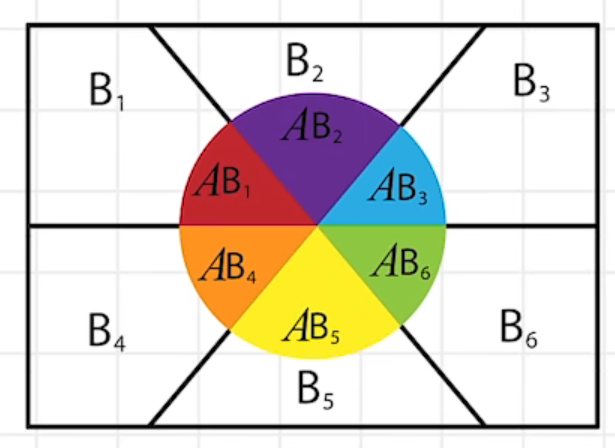
\includegraphics[width=0.3\textwidth,center]{../photo/quangailv.png}
\subsubsection{独立性}
\indent若事件$AB$独立,则$P(AB)=P(A)P(B),P(B)=P(B|A)=P(B|\overline{A})$。\\
\indent$A$和$B$互相独立,则$A$和$\overline{B}$,$\overline{A}$和$B$,$\overline{A}$和$\overline{B}$也互相独立。\\
\subsubsection{随机变量}
\indent对于随机变量$X$,称函数$F(X)=P(X\leq x)$为$X$的\textbf{分布函数},分布函数单调递增,$F(-\infty)=0,F(\infty)=1$。\\
\noindent\textbf{离散型随机变量}\\
\indent分布函数:$F(X)=\displaystyle\sum_{x_{k}\leq x}p_k$\\
\noindent\textbf{连续型随机变量}\\
\indent分布函数:$F(x)=\int_{-\infty}^{x}f(t)\text{d}t$,同样的$\int_{-\infty}^{\infty}f(t)\text{d}t=1$\\
\indent概率密度:$f(x)=F^{\prime}(x)$
\subsubsection{二项分布与泊松分布}
\indent二项分布:$P\{X=k\}=C_n^{k} p^{k} q^{n-k}(q=1-p)$\\
\indent泊松分布:$P\{X=k\}=\frac{\lambda^{k}e^{-\lambda}}{k!}$
\subsubsection{正态分布}
$X\sim N(\mu,\sigma^2)$其中$\mu$是期望,$\sigma^2$是方差。\\
\indent方差:$D(X)=E(X^2)-[E(x)]^2$。标准差$\sigma=\sqrt{D(x)}$
\subsubsection{期望}
\indent离散型随机变量的期望:$E(X)=\displaystyle\sum_{i=1}^{\infty}x_i p_i$\\
\indent连续型随机变量的期望:$E(X)=\int_{-\infty}^{\infty}xf(x)\text{d}x$\\
\indent$E(CX)=CE(X),E(X+Y)=E(X)+E(Y)$\\
\indent设$X,Y$互相独立,则$E(XY)=E(X)E(Y)$


\section{高精度算法}
\begin{lstlisting}[language=c++]
const int maxn = 1000;//maxn越大速度越慢
struct bign{
    int d[maxn], len;
    void clean() { while(len > 1 && !d[len-1]) len--; }
    bign() { memset(d, 0, sizeof(d)); len = 1; }
    bign(int num) { *this = num; } 
    bign(char* num) { *this = num; }
    bign operator = (const char* num){
        memset(d, 0, sizeof(d)); len = strlen(num);
        for(int i = 0; i < len; i++) d[i] = num[len-1-i] - '0';
        clean();
        return *this;
    }
    bign operator = (int num){
        char s[20]; sprintf(s, "%d", num);
        *this = s;
        return *this;
    }

    bign operator + (const bign& b){
        bign c = *this; int i;
        for (i = 0; i < b.len; i++){
            c.d[i] += b.d[i];
            if (c.d[i] > 9) c.d[i]%=10, c.d[i+1]++;
        }
        while (c.d[i] > 9) c.d[i++]%=10, c.d[i]++;
        c.len = max(len, b.len);
        if (c.d[i] && c.len <= i) c.len = i+1;
        return c;
    }
    bign operator - (const bign& b){
        bign c = *this; int i;
        for (i = 0; i < b.len; i++){
            c.d[i] -= b.d[i];
            if (c.d[i] < 0) c.d[i]+=10, c.d[i+1]--;
        }
        while (c.d[i] < 0) c.d[i++]+=10, c.d[i]--;
        c.clean();
        return c;
    }
    bign operator * (const bign& b)const{
        int i, j; bign c; c.len = len + b.len; 
        for(j = 0; j < b.len; j++) for(i = 0; i < len; i++) 
            c.d[i+j] += d[i] * b.d[j];
        for(i = 0; i < c.len-1; i++)
            c.d[i+1] += c.d[i]/10, c.d[i] %= 10;
        c.clean();
        return c;
    }
    bign operator / (const bign& b){
        int i, j;
        bign c = *this, a = 0;
        for (i = len - 1; i >= 0; i--)
        {
            a = a*10 + d[i];
            for (j = 0; j < 10; j++) if (a < b*(j+1)) break;
            c.d[i] = j;
            a = a - b*j;
        }
        c.clean();
        return c;
    }
    bign operator % (const bign& b){
        int i, j;
        bign a = 0;
        for (i = len - 1; i >= 0; i--)
        {
            a = a*10 + d[i];
            for (j = 0; j < 10; j++) if (a < b*(j+1)) break;
            a = a - b*j;
        }
        return a;
    }
    bign operator += (const bign& b){
        *this = *this + b;
        return *this;
    }

    bool operator <(const bign& b) const{
        if(len != b.len) return len < b.len;
        for(int i = len-1; i >= 0; i--)
            if(d[i] != b.d[i]) return d[i] < b.d[i];
        return false;
    }
    bool operator >(const bign& b) const{return b < *this;}
    bool operator<=(const bign& b) const{return !(b < *this);}
    bool operator>=(const bign& b) const{return !(*this < b);}
    bool operator!=(const bign& b) const{return b < *this || *this < b;}
    bool operator==(const bign& b) const{return !(b < *this) && !(b > *this);}

    string str() const{
        char s[maxn]={};
        for(int i = 0; i < len; i++) s[len-1-i] = d[i]+'0';
        return s;
    }
};
istream& operator >> (istream& in, bign& x)
{
    string s;
    in >> s;
    x = s.c_str();
    return in;
} 
ostream& operator << (ostream& out, const bign& x)
{
    out << x.str();
    return out;
}
int main()
{
    bign a, b;
    while (cin >> a >> b) cout << a+b << endl;
    return 0;
}
\end{lstlisting}
\ifx\allfiles\undefined
\end{document}
\fi


    \chapter{图论}
    \ifx\allfiles\undefined
\documentclass[a4paper]{book}
\usepackage{ctex}
\usepackage{graphicx} %插入图片
\usepackage{amsmath,amsthm}
\usepackage{lmodern}
\usepackage{float}
\usepackage[export]{adjustbox}
\usepackage{listings,xcolor} %代码块
\usepackage{amssymb}
\usepackage{xcolor}
\usepackage{listings}
\lstset{
    breaklines,                                 % 自动将长的代码行换行排版
    extendedchars=false,                        % 解决代码跨页时,章节标题,页眉等汉字不显示的问题
    backgroundcolor=\color[rgb]{0.96,0.96,0.96},% 背景颜色
    keywordstyle=\color{blue}\bfseries,         % 关键字颜色
    identifierstyle=\color{black},              % 普通标识符颜色
    commentstyle=\color[rgb]{0,0.6,0},          % 注释颜色
    stringstyle=\color[rgb]{0.58,0,0.82},       % 字符串颜色
    showstringspaces=false,                     % 不显示字符串内的空格
    numbers=left,                               % 显示行号
    numberstyle=\small\ttfamily,                % 设置数字字体
    basicstyle=\small\ttfamily,                 % 设置基本字体
    captionpos=t,                               % title在上方(在bottom即为b)
    frame=single,                               % 设置代码框形式
    rulecolor=\color[rgb]{0.8,0.8,0.8},         % 设置代码框颜色
}  
   

\begin{document}
\fi

\section{图的存储}

\subsection{链式前向星}

\begin{lstlisting}[language=C++]
struct road{int b,c,nex;}r[2000005];
void add(int a,int b,int c)
{
    r[num].b=b;r[num].c=c;
    r[num].nex=head[a];head[a]=num++;
}
\end{lstlisting}

\section{树}
\subsection{树的直径}
\noindent\textbf{求法:}\\
\indent1.两次$\mathrm{DFS}$,第一次从任意点出发,找到距离最远的点$x$。第二次从$x$出发,找到的最远点$y$。此方法不适用于有负权边的树。\\
\indent2.树形$\mathrm{DP}$,求出$x$子树中最深的深度和次深的深度,最大的和即为直径。\\
\noindent\textbf{性质:}\\
\indent1.从树上任一点出发,在树上的最长路径距离一定是到直径两端点中的一个。\\
\indent2.若树上所有边边权均为正,则树的所有直径中点重合。
\begin{lstlisting}[language=C++,title=方法1]
void dfs(int u,int fa)
{
    for(int i=0;i<v[u].size();i++)
    {
        int nex=v[u][i];
        if(nex==fa) continue;
        dep[nex]=dep[u]+1;
        if(dep[nex]>dep[t]) t=nex;
        dfs(nex,u);
    }
}
\end{lstlisting}
\begin{lstlisting}[language=C++,title=方法2]
void dfs(int u,int fa) 
{
    d1[u]=d2[u]=0;
    for(auto nex:v[u]) 
    {
        if(nex==fa) continue;
        dfs(nex,u);
        int t=d1[nex]+1;
        if(t>d1[u]) d2[u]=d1[u],d1[u]=t;
        else if(t>d2[u]) d2[u]=t;
    }
    d=max(d,d1[u]+d2[u]);
}
\end{lstlisting}


\subsection{树的重心}
\noindent将树的某点删掉后,会形成有多棵树的森林,可以使森林中最大的树最小的点就是树的重心。\\
\noindent\textbf{性质:}\\
\indent1.以树的重心为根时,所有子树的大小都不超过整棵树大小的一半。\\
\indent2.树中所有点到某个点的距离和中,到重心的距离和是最小的;如果有两个重心,那么到它们的距离和一样。\\
\indent3.树中所有点到某个点的距离和中,到重心的距离和是最小的;如果有两个重心,那么到它们的距离和一样。\\
\indent4.在一棵树上添加或删除一个叶子,那么它的重心最多只移动一条边的距离。\\
\indent5.一棵树最多有两个重心,且相邻。\\
\noindent\textbf{求法:}\\
\indent$\mathrm{DFS}$计算每个子树的大小,记录“向下”的子树的最大大小,利用总点数-当前子树(这里的子树指有根树的子树)的大小得到“向上”的子树的大小,然后就可以依据定义找到重心了。
\begin{lstlisting}[language=C++]
void dfs(int u,int fa)
{
    sz[u]=1;
    for(int i=0;i<v[u].size();i++)
    {
        int nex=v[u][i];
        if(nex==fa) continue;
        dfs(nex,u);
        sz[u]+=sz[nex];
        w[u]=max(w[u],sz[nex]);
    }
    w[u]=max(w[u],n-sz[u]);
}
\end{lstlisting}

\paragraph{带权树重心\\}
树上点具有点权,重心到所有点的距离乘各点点权的乘积之和最小。
\begin{lstlisting}[language=C++,escapeinside=``]
//`w[i]代表i点的权值,f[i]代表以i点为跟产生的重量大小`
void dfs(int u,int fa)
{
    sz[u]+=w[u];
    for(int i=0;i<v[u].size();i++)
    {
        int nex=v[u][i];
        if(nex==fa) continue;
        dep[nex]=dep[u]+1;
        dfs(nex,u);
        sz[u]+=sz[nex];
    }
    f[1]+=w[u]*dep[u];
}
void dfs2(int u,int fa)
{
    for(int i=0;i<v[u].size();i++)
    {
        int nex=v[u][i];
        if(nex==fa) continue;
        f[nex]=f[u]+sz[1]-sz[nex]*2;
        dfs2(nex,u);
    }
}
\end{lstlisting}
\subsection{最近公共祖先}
\begin{lstlisting}[language=c++]
void dfs(int u,int fa)//fa=0
{
    f[u][0]=fa;dep[u]=dep[fa]+1;
    for(int i=1;i<=20;i++) f[u][i]=f[f[u][i-1]][i-1];
    for(int i=head[u];~i;i=r[i].nex)
    {
        int nx=r[i].b;
        if(nx==fa) continue;
        dfs(nx,u);
    }
}
int lca(int a,int b)
{
    if(dep[a]<dep[b]) swap(a,b);
    for(int i=20;i>=0;i--)
    {
        if(dep[f[a][i]]>=dep[b]) a=f[a][i];
    }
    if(a==b) return a;
    for(int i=20;i>=0;i--)
    {
        if(f[a][i]!=f[b][i]) a=f[a][i],b=f[b][i]; 
    }
    return f[a][0];
}
\end{lstlisting}
\subsection{树上启发式合并}
\noindent\textbf{时间复杂度证明:}\\
\indent一个有$n$个结点的树,根节点到任意一点经过的轻边数量小于$\log n$ 条。一个节点的被遍历的次数等于它到根节点路径上的轻边数$+1$,所以一个节点的被遍历次数$\log n+1$,总时间复杂度则为$O(n(\log n+1))=O(n\log n)$。
\begin{lstlisting}[language=C++,title=树上启发式合并求子树中颜色种类]
void add(int u){if(vis[col[u]]==0) num++;vis[col[u]]++;}
void del(int u){if(vis[col[u]]==1) num--;vis[col[u]]--;}
void dfs(int u,int fa)
{
    sz[u]=1;L[u]=++dfn;pos[dfn]=u;R[u]=dfn;
    int mx=0;
    for(auto nex:v[u])
    {
        if(nex==fa) continue;
        dfs(nex,u);
        sz[u]+=sz[nex];R[u]=max(R[u],R[nex]);
        if(sz[nex]>mx) mx=sz[nex],big[u]=nex;
    }
}
void dfs2(int u,int fa,int lable)
{
    for(auto nex:v[u])
    {
        if(nex==fa || nex==big[u]) continue;
        dfs2(nex,u,0);
    }
    if(big[u]) dfs2(big[u],u,1);
    add(u);
    for(auto nex:v[u])
    {
        if(nex==fa || nex==big[u]) continue;
        for(int i=L[nex];i<=R[nex];i++) add(pos[i]);
    }
    ans[u]=num;
    if(lable==0) 
    {
        for(int i=L[u];i<=R[u];i++) del(pos[i]);
    } 
}
\end{lstlisting}

\subsection{虚树}
$[4,6,7]$三点构成的虚树如图。使用虚树可以缩小树形$DP$遍历的范围。\\
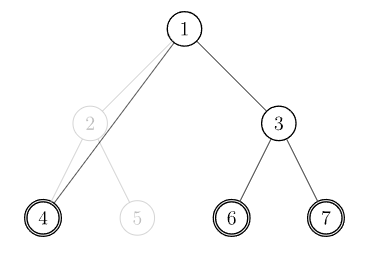
\includegraphics[width=0.5\textwidth,center]{../photo/VirtualTree}
\begin{lstlisting}[language=C++,escapeinside=``]
bool cmp(int a,int b){return dfn[a]<dfn[b];};
void dfs(int u,int fa)
{
    dfn[u]=++tim;f[u][0]=fa;dep[u]=dep[fa]+1;
    for(int i=1;i<20;i++) f[u][i]=f[f[u][i-1]][i-1];
    for(int i=head[u];~i;i=r[i].nex)
    {
        int nex=r[i].b;
        if(nex==fa) continue;
        dfs(nex,u);
    }
}
int lca(int a,int b)
{
    if(dep[a]<dep[b]) swap(a,b);
    for(int i=19;i>=0;i--)
    {
        if(dep[f[a][i]]>=dep[b])
        a=f[a][i];
    }
    if(a==b) return a;
    for(int i=19;i>=0;i--)
    {
        if(f[a][i]!=f[b][i])
        a=f[a][i],b=f[b][i]; 
    }
    return f[a][0];
}
void build_Virtual_Tree(int rt)
{
    sort(h.begin(),h.end(),cmp);
    //切记不要拿出来清空,警钟敲烂
    sta[top=1]=rt;vtree[rt].clear();
    for(int i=0;i<h.size();i++)
    {
        if(h[i]==rt) continue;
        int l=lca(sta[top],h[i]);
        //`LCA与栈顶不同,说明当前节点与栈中节点不在同一条树链上`
        if(l!=sta[top]) 
        {
            //`找到栈中与当前LCA在同一树链上的位置`
            while(dfn[sta[top-1]]>dfn[l]) 
            {
                vtree[sta[top-1]].push_back(sta[top]);
                top--;
            }
            //`这个位置不是LCA,将LCA入栈`
            if(dfn[l]>dfn[sta[top-1]]) 
            {
                vtree[l].clear();
                vtree[l].push_back(sta[top]);sta[top]=l;
            }
            else //`LCA就在栈中`
            {
                vtree[l].push_back(sta[top--]);
            }
        }
        sta[++top]=h[i];vtree[h[i]].clear();
    }
    for(int i=1;i<top;i++) 
    {
        vtree[sta[i]].push_back(sta[i+1]);
    }
}
\end{lstlisting}
\subsection{树分治}
\subsubsection{点分治}
\begin{lstlisting}[language=c++,escapeinside=``,title=求出树上两点距离小于等于$k$的点对数量]
#include<bits/stdc++.h>
using namespace std;
const int maxn=4e4+7;
int num,head[maxn],n,m,sz[maxn],w[maxn],rt,vis[maxn],dis[maxn],sum,k;
struct road{int b,c,nex;}r[80005];
void add(int a,int b,int c)
{
    r[num].b=b;r[num].c=c;r[num].nex=head[a];head[a]=num++;
}
void getrt(int u,int fa)//`找u子树中的重心`
{
    sz[u]=1;w[u]=0;
    for(int i=head[u];~i;i=r[i].nex)
    {
        int nex=r[i].b;
        if(nex==fa||vis[nex]) continue;
        getrt(nex,u);
        sz[u]+=sz[nex];
        w[u]=max(w[u],sz[nex]);
    }
    w[u]=max(w[u],sum-sz[u]);
    if(w[u]<w[rt]) rt=u;
}
int ans,cnt,a[maxn],b[maxn];
void dfs(int u,int fa,int dis,int from)
{
    b[u]=dis;a[++cnt]=b[u];
    for(int i=head[u];~i;i=r[i].nex)
    {
        int nex=r[i].b;
        if(nex==fa||vis[nex]) continue;
        dfs(nex,u,dis+r[i].c,from);
    }
}
int caldis(int u,int dis)
{
    cnt=0;b[u]=dis;a[++cnt]=b[u];
    for(int i=head[u];~i;i=r[i].nex)
    {
        int nex=r[i].b;
        if(vis[nex]) continue;
        dfs(nex,u,r[i].c+dis,nex);
    }
    int res=0;
    sort(a+1,a+1+cnt);
    for(int i=1,j=cnt;i<j;i++)
    {
        while((j-1)>i&&a[j]+a[i]>k) j--;
        if(j>i&&a[j]+a[i]<=k) res+=(j-i);
    }
    return res;
}
void solve(int u)
{
    vis[u]=1;ans+=caldis(u,0);
    for(int i=head[u];~i;i=r[i].nex)
    {
        int nex=r[i].b;
        if(vis[nex]) continue;
        ans-=caldis(nex,r[i].c);
        dis[nex]=r[i].c;
        rt=0;sum=sz[nex];
        getrt(nex,u);solve(rt);
    }
}
int main()
{
    memset(head,-1,sizeof(head));
    scanf("%d",&n);
    for(int i=1;i<n;i++)
    {
        int a,b,c;scanf("%d%d%d",&a,&b,&c);
        add(a,b,c);add(b,a,c);
    }
    scanf("%d",&k);
    w[rt]=1e9;sum=n;getrt(1,0);solve(rt);
    printf("%d\n",ans);
}
\end{lstlisting}
\section{生成树}

\subsection{次小生成树}
\noindent最小生成树转变为次小生成树,只需要插入一条新边,删去一条原边即可。\\
\noindent枚举可以插入的新边,在新边LCA的路径上找到可以删去的最长的边,可以用倍增实现。
\begin{lstlisting}[language=C++]
#include<bits/stdc++.h>
#define int long long
#define pb push_back
using namespace std;
const int maxn=3e5+7;
struct road{int x,y,c;}r[maxn];
bool cmp(road a,road b){return a.c<b.c;}
int n,m,vis[maxn],fa[maxn];
int find(int x){return fa[x]==x?x:fa[x]=find(fa[x])}
vector<pair<int,int>>v[maxn];
int f[maxn][20],mx1[maxn][20],mx2[maxn][20],depth[maxn];
void dfs(int u,int fa)
{
    depth[u]=depth[fa]+1;
    f[u][0]=fa;
    for(int i=0;i<v[u].size();i++)
    {
        auto nex=v[u][i];
        if(nex.first==fa) continue;
        mx1[nex.first][0]=nex.second;
        mx2[nex.first][0]=-1e18;
        dfs(nex.first,u);
    }
}
void ST()
{
    for(int i=1;i<20;i++)
    {
        for(int j=1;j<=n;j++)
        {
            f[j][i]=f[f[j][i-1]][i-1];
            mx1[j][i]=max(mx1[j][i-1],mx1[f[j][i-1]][i-1]);
            mx2[j][i]=max(mx2[j][i-1],mx2[f[j][i-1]][i-1]);
            if(mx1[j][i-1]!=mx1[f[j][i-1]][i-1]) 
            mx2[j][i]=max(mx2[j][i],min(mx1[j][i-1],mx1[f[j][i-1]][i-1]));
        }
    }
}
int LCA(int a,int b)
{
    if(depth[a]<depth[b]) swap(a,b);
    for(int i=19;i>=0;i--)
    {
        if(depth[f[a][i]]>=depth[b]) a=f[a][i];
    }
    if(a==b) return a;
    for(int i=19;i>=0;i--)
    {
        if(f[a][i]!=f[b][i]) a=f[a][i],b=f[b][i]; 
    }
    return f[a][0];
}
int findmx(int x,int pa,int val)
{
    int len=-1e18;
    for(int i=19;i>=0;i--)
    {
        if(depth[f[x][i]]<depth[pa]) continue;
        if(mx1[x][i]!=val) len=max(len,mx1[x][i]);
        else len=max(len,mx2[x][i]);
        x=f[x][i];
    }
    return len;
}
signed main()
{
    scanf("%lld%lld",&n,&m);
    for(int i=1;i<=n;i++) fa[i]=i;
    for(int i=1;i<=m;i++)
    {
        scanf("%lld%lld%lld",&r[i].x,&r[i].y,&r[i].c);
    }
    sort(r+1,r+1+m,cmp);
    int sum=0;
    for(int i=1;i<=m;i++)
    {
        int px=find(r[i].x),py=find(r[i].y);
        if(px==py) continue;
        vis[i]=1;fa[px]=py;sum+=r[i].c;
        v[r[i].x].pb({r[i].y,r[i].c});v[r[i].y].pb({r[i].x,r[i].c});
    }
    dfs(1,0);
    ST();
    int ans=1e18;
    for(int i=1;i<=m;i++)
    {
        if(vis[i]) continue;
        int lca=LCA(r[i].x,r[i].y);
        int lmx=findmx(r[i].x,lca,r[i].c),rmx=findmx(r[i].y,lca,r[i].c); 
        ans=min(ans,sum-max(lmx,rmx)+r[i].c);
    }
    printf("%lld\n",ans);
}
\end{lstlisting}
\subsection{瓶颈生成树}
\noindent定义:\\
\indent无向图G的瓶颈生成树是这样的一个生成树,它的最大的边权值在$G$的所有生成树中最小。\\
\noindent性质:\\
\indent\textbf{最小生成树是瓶颈生成树的充分不必要条件。}即最小生成树一定是瓶颈生成树,而瓶颈生成树不一定是最小生成树。
\subsubsection{最小瓶颈路}
\indent无向图$G$中$x$到$y$的最小瓶颈路是这样的一类简单路径,满足这条路径上的最大的边权在所有$x$到$y$的简单路径中是最小的。\\
\noindent性质:\\
\indent $x$到$y$的最小瓶颈路上的最大边权等于最小生成树上$x$到$y$路径上的最大边权。
\subsection{Kruskal重构树}
\noindent构造方法:\\
\indent在跑Kruskal的过程中我们会从小到大加入若干条边,现在我们仍然按照这个顺序。
每一次加边会合并两个集合,我们可以新建一个点,点权为加入边的边权,同时将两个集合的根节点分别设为新建点的左儿子和右儿子。
然后我们将两个集合和新建点合并成一个集合,将新建点设为根。\\
\indent不难发现,在进行$n-1$轮之后我们得到了一棵恰有$2n-1$个节点的二叉树,同时每个非叶子节点恰好有两个儿子。这棵树就叫Kruskal重构树。\\
\noindent性质:\\
\indent两点的LCA的点权为原图中最大值最小的路径上的最大值(最小瓶颈路)。\\
\indent是一颗二叉树,任意点的权值大于左右儿子的权值,是一个大根堆。\\
\\
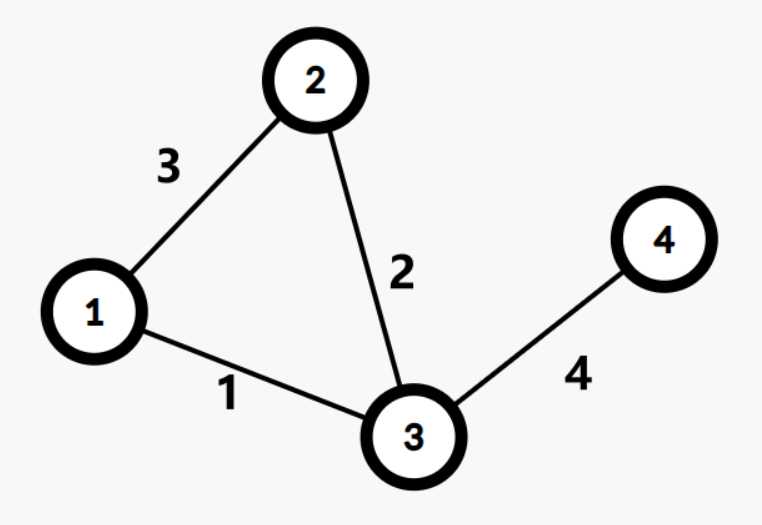
\includegraphics[width=0.5\textwidth]{../photo/kru1}
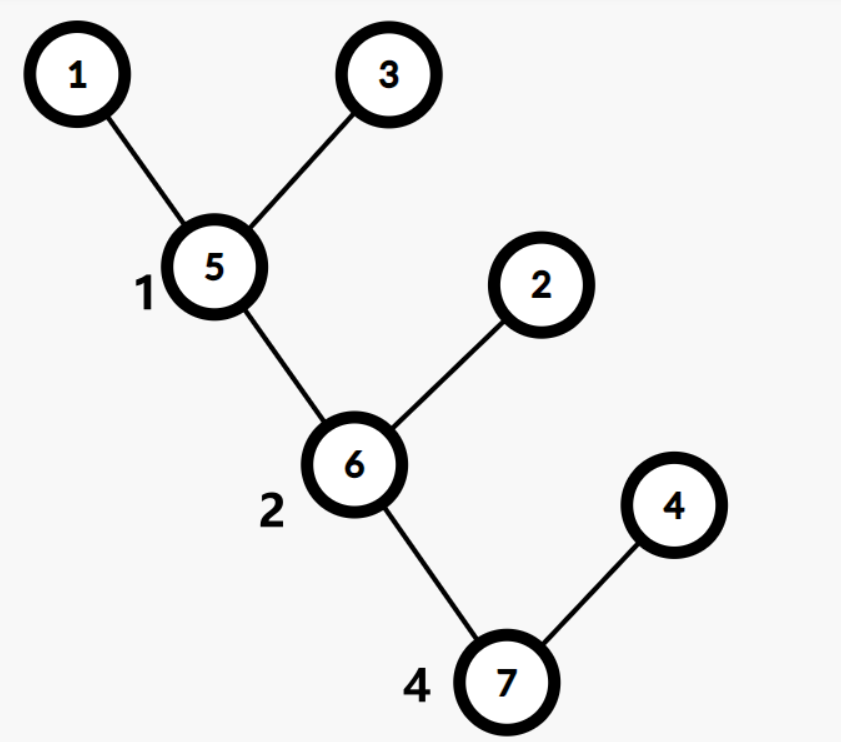
\includegraphics[width=0.5\textwidth]{../photo/kru2}
\begin{center}
    左为原图,右为该图的Kruskal重构树
\end{center}
\begin{lstlisting}[language=C++]
void Kruskal()
{
    sort(r+1,r+1+m,cmp);
    for(int i=1;i<=m;i++)
    {
        int px=find(r[i].x),py=find(r[i].y);
        if(px==py) continue;
        fa[px]=fa[py]=++idx;fa[idx]=idx;
        val[idx]=r[i].c;
        add(idx,px);add(idx,py);
    }
}
\end{lstlisting}
\section{最小树形图}
\noindent有向图上的最小生成树称为最小树形图。
\subsection{朱刘算法}
\noindent\textbf{求DAG上最小树形图:}\\
\indent对于一个$DAG$,只要我们对于每一个点选出最小的入边,那么这一定是个树形图。\\
\noindent\textbf{求环上最小树形图:}\\
\indent只需要将环上最长的一条边去掉即可。\\
\noindent\textbf{求有向图最小树形图:}\\
\indent对图上所有点直接选取其最小的入边,判断这些边是组成环。\\
\indent若无环,说明已经找到了最小树形图,直接结束即可。\\
\indent若有环,肯定要把其中一条边换成环外边。我们就把贪心算出来的那个所谓的“树形图”上的环\textbf{缩成一个点},环外边指向这个所称的点,为了方便统计,由于我们确信环外边的长度$\ge$环内边的长度,那么我们ans先加上这个环的边权和,然后指向环的边边权设为:\textbf{自己的长度$-$所连向的环内点在环中指向的点的边的长度}。\\
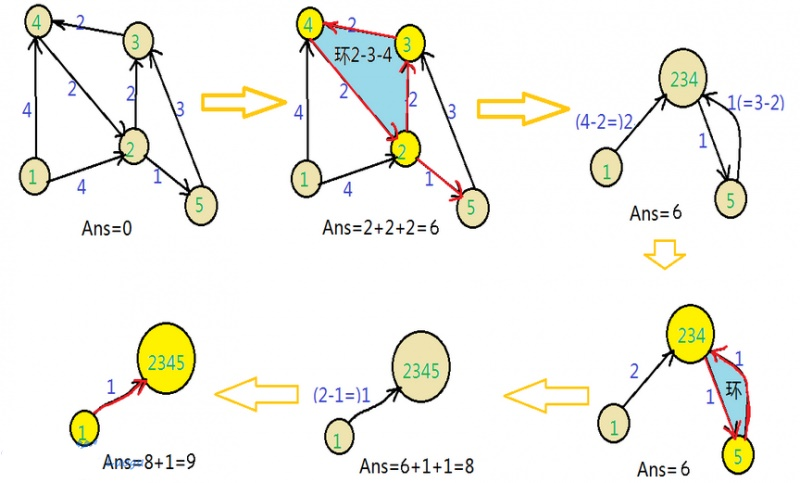
\includegraphics[width=0.8\textwidth,center]{../photo/zl.jpg}\\
\indent这样我们一直加边,找环,缩点循环,直到找到的是一个$DAG$。至此结束,时间复杂度$O(nm)$。
\begin{lstlisting}[language=c++,escapeinside=``]
int Edmonds(int root)
{
    int ans=0,cnt=0;
    while(1)
    {	//`i点的父亲是fa[i],祖先是top[i],属于第loop[i]个环,其选择的入边权值为mn[i]`
        for(int i=1;i<=n;i++) fa[i]=top[i]=loop[i]=0,mn[i]=1e9;
        for(int i=1;i<=m;i++) //找每个点最小的入边
        {
            int u=e[i].u,v=e[i].v,w=e[i].w;
            if(u!=v&&w<mn[v]) mn[v]=w,fa[v]=u;
        }
        mn[root]=0;
        for(int i=1;i<=n;i++) 
        {
            if(mn[i]==1e9) return -1; //有点无边连接,无解
            ans+=mn[i];
        }
        for(int i=1,j=1;i<=n;i++,j=i)
        {
            while(j!=root&&top[j]!=i&&!loop[j]) top[j]=i,j=fa[j];
            if(j!=root&&!loop[j]) //找到环,标号
            {
                loop[j]=++cnt;
                for(int k=fa[j];k!=j;k=fa[k]) loop[k]=cnt;
            }
        }
        if(!cnt) return ans; //如果无环,结束
        for(int i=1;i<=n;i++) if(!loop[i]) loop[i]=++cnt;//将不在环内的点设置为独立环
        for(int i=1;i<=m;i++) //缩点并且重新设置新边权
            e[i].w-=mn[e[i].v],e[i].u=loop[e[i].u],e[i].v=loop[e[i].v];
        n=cnt;root=loop[root];cnt=0; //`初始化。注意会更改n的值!!!!`
    }
}
\end{lstlisting}
\section{斯坦纳树}
\subsubsection{最小斯坦纳树}
给定连通图$G$中的$n$个点与$k$个关键点,连接$k$个关键点,使得生成树的所有边的权值和最小。\\
我们使用状态压缩动态规划来求解。用$f(i,S)$表示以$i$为根的一棵树,包含集合$S$中所有点的最小边权值和。
\begin{enumerate}
    \item 对于$i$的度数为$1$的情况,可以考虑枚举树上与$i$相邻的点$j$,则:$f(i,S)=f(j,S)+w(j,i)$。
    \item 对于$i$的度数大于$1$的情况,可以划分成几个子树考虑,即:$f(i,S)=f(i,T)+f(i,S-T)$。
\end{enumerate}
时间复杂度为$O(n\times 3^k+m\log m\times 2^k)$。
\begin{lstlisting}[language=c++]
#include<bits/stdc++.h>
using namespace std;
const int maxn=105;
typedef pair<int,int> PII;
int head[maxn],num,f[maxn][(1<<10)+5],key[10],vis[maxn];
struct road{int b,c,nex;}r[10005];
void add(int a,int b,int c)
{r[num].b=b;r[num].c=c;r[num].nex=head[a];head[a]=num++;}
priority_queue<PII,vector<PII>,greater<PII>>q;
void dijkstra(int s)
{
    memset(vis,0,sizeof(vis));
    while(!q.empty())
    {
        auto [val,u]=q.top();q.pop();
        if(vis[u]) continue;
        vis[u]=1;
        for(int i=head[u];~i;i=r[i].nex)
        {
            int v=r[i].b;
            if(f[v][s]>f[u][s]+r[i].c)
            {
                f[v][s]=f[u][s]+r[i].c;
                q.push({f[v][s],v});
            }
        }
    }
}
int main()
{
    memset(f,0x3f,sizeof(f));
    memset(head,-1,sizeof(head));
    int n,m,k;scanf("%d%d%d",&n,&m,&k);
    for(int i=1;i<=m;i++)
    {
        int a,b,c;scanf("%d%d%d",&a,&b,&c);
        add(a,b,c);add(b,a,c);
    }
    for(int i=1;i<=k;i++)
    {
        scanf("%d",&key[i]);f[key[i]][1<<(i-1)]=0;
    }
    for(int i=1;i<(1<<k);i++)
    {
        for(int j=1;j<=n;j++)
        {
            for(int sub=i&(i-1);sub;sub=i&(sub-1))
            {
                f[j][i]=min(f[j][i],f[j][sub]+f[j][i^sub]);
            }
            if(f[j][i]!=0x3f3f3f3f) q.push({f[j][i],j});
        }
        dijkstra(i);
    }
    printf("%d\n",f[key[1]][(1<<k)-1]);
}
\end{lstlisting}
\section{基环树}
\indent如果一张无向连通图包含恰好一个环,则称它是一棵基环树。\\
\indent如果一张有向弱连通图每个点的入度都为$1$,则称它是一棵基环外向树。\\
\indent如果一张有向弱连通图每个点的出度都为$1$,则称它是一棵基环内向树。
\begin{enumerate}
    \item 先处理环上每个点支出来的子树部分,然后把贡献记录在环上的点,最后问题就成了计算一个环的答案了。
    \item 先删去环上的一条边,让基环树变成真正的树计算后考虑加上之前删去那条边的影响即可(使用并查集找到环上的两个点,以两个点为树根分别树形DP)。
\end{enumerate}
\subsubsection{基环树直径}
\indent基环树的直径显然有下面两种可能:1.在“根节点”的某一棵子树中。2.经过“根节点”,在“根节点”的某两棵子树中。\\
\indent先将基环树中的环剔出来,对于环上的每棵树,使用动态规划法求出树的直径,即可解决1的可能。对于2,我们需要找到环上的两个节点$i,j$,使得$d_i+d_j+dist_{i,j}$最大。这需要我们将长度为$n$的环拓展为长度为$2*n$的链,使用单调队列维护最大的$d_j+dist_{i,j}$即可。
\begin{lstlisting}[language=c++,title=IOI2008-Island,escapeinside=``]
#include<bits/stdc++.h>
#define int long long
using namespace std;
const int maxn=1e6+7;
int head[maxn],num,n,vis[maxn],loop[2*maxn],cnt,lable[maxn],s[2*maxn];
struct road{int b,c,nex;}r[2000005];
void add(int a,int b,int c)
{
    r[num].b=b;r[num].c=c;r[num].nex=head[a];head[a]=num++;
}
bool dfs(int u,int f)
{
    if(vis[u]==1)
    {
        vis[u]=2,loop[++cnt]=u,lable[u]=1;
        return 1;
    }//找到衔接点
    vis[u]=1; //维护访问数组
    for(int i=head[u];~i;i=r[i].nex)
    {
        if(i!=(f^1)&&dfs(r[i].b,i))//如果当前边不是上一条边并且当前节点在环上
        {
            if(vis[u]!=2)//当前节点不是衔接点
            {
                loop[++cnt]=u,lable[u]=1,s[cnt]=r[i].c;
                return 1;
            } 
            else//是衔接点
            {
                s[1]=r[i].c;
                return 0;
            }
        }
    }
    return 0;	
}
int d1[maxn],d2[maxn],d;
void dfs2(int u,int fa)
{
    d1[u]=d2[u]=0;vis[u]=1;
    for(int i=head[u];~i;i=r[i].nex) 
    {
        int nex=r[i].b;
        if(nex==fa||lable[nex]) continue;
        dfs2(nex,u);
        int t=d1[nex]+r[i].c;
        if(t>d1[u]) d2[u]=d1[u],d1[u]=t;
        else if(t>d2[u]) d2[u]=t;
    }
    d=max(d,d1[u]+d2[u]);
}
signed main()
{
    memset(head,-1,sizeof(head));
    scanf("%lld",&n);
    for(int i=1;i<=n;i++)
    {
        int a,b;scanf("%lld%lld",&a,&b);
        assert(a!=i);
        add(i,a,b);add(a,i,b);
    }
    int ans=0;
    for(int i=1;i<=n;i++)
    {
        if(vis[i]) continue;
        cnt=0;dfs(i,-1);
        int sum=0;
        for(int j=1;j<=cnt;j++)
        {
            d=0;dfs2(loop[j],-1);
            sum=max(sum,d);
            s[j+cnt]=s[j];loop[j+cnt]=loop[j];
        }
        s[1]=0;
        for(int j=2;j<=2*cnt;j++) s[j]=s[j-1]+s[j];
        deque<int>q;
        for(int j=1;j<=2*cnt;j++)
        {
            while(!q.empty()&&q.front()<=j-cnt+1) q.pop_front();
            while(!q.empty()&&s[q.back()]+d1[loop[q.back()]]<=s[j]+d1[loop[j]]) 
            q.pop_back();
            q.push_back(j);
            if(j>=cnt) 
            {
                int u=q.front();
                sum=max(sum,s[u]-s[j-cnt+1]+d1[loop[u]]+d1[loop[j-cnt+1]]);
            }
        }
        ans+=sum;
    }
    printf("%lld\n",ans);
}
\end{lstlisting}
\section{搜索}
\subsection{双向搜索}
\subsubsection{双向同时搜索}
双向同时搜索的基本思路是从状态图上的起点和终点同时开始进行广搜或深搜。将起点和终点位置分别打上不同的标记,并使用搜索拓展,若某次拓展过程中遇到了不同的标记,则搜索的两端相遇了,那么可以认为是获得了可行解。
\subsubsection{meet in the middle}
主要思想是将整个搜索过程分成两半,分别搜索,最后将两半的结果合并。\\
\indent暴力搜索的时间复杂度往往是指数级别的,而改用meet in the middle算法后复杂度的指数可以减半,即让复杂度从$O(a^b)$降低成$O(a^{b/2})$。\\
\indent使用DFS同时维护模式,状态,步数基本可以较为简单的实现。
\subsection{0-1BFS}
本质是dijkstra算法,图上的边权有$0,1$两种。使用双端队列进行BFS,队首一定是队列中距离起点距离最短的点,走距离为$0/1$的边时分别将新的位置加入队首/队尾,以此来实现最短路中的松弛操作。
\subsection{A*}
A*算法是一种以BFS为基础的优化算法,在起点到终点的广阔搜索范围中,我们可以通过定义合理的启发式函数,缩小搜索的范围,从而加速搜索。\\
\indent定义起点为$s$,终点为$t$,从起点(初始状态)开始的真实距离为$d(x)$,到终点(最终状态)的真实距离$h(x)$,估计距离为$h^{*}(x)$,必须满足$h^{*}(x)\leq h(x)$,以及每个点的估价函数$f(x)=d(x)+h^{*}(x)$。\\
\indent A*算法每次从优先队列中取出一个$f$最小的元素,然后更新相邻的状态。在启发式函数的约束下,搜索效率得以提升,当\textbf{终点第一次离开队列时},此时记录的便是最优答案。\\
\indent当$h=0$时,A*算法变为 Dijkstra,当$h=0$并且边权为$1$时变为BFS。
\subsubsection{八数码问题}
\indent题目大意:在$3\times3$的棋盘上,摆有八个棋子,每个棋子上标有$1$至$8$的某一数字。棋盘中留有一个空格,空格用$0$来表示。空格周围的棋子可以移到空格中,这样原来的位置就会变成空格。给出一种初始布局和目标布局(为了使题目简单,设目标状态如下),找到一种从初始布局到目标布局最少步骤的移动方法。\\
\indent启发式函数$h$定义为,不在应该在的位置的数字个数。
\begin{lstlisting}[language=C++]
#include<bits/stdc++.h>
using namespace std;
string ed="123804765",st;
int h(string s)
{
    int cnt=0;
    for(int i=0;i<9;i++) cnt+=(s[i]!=ed[i]);
    return cnt;
}
map<string,int>vis;
int nex[4]={-3,3,-1,1};
struct node
{
    string str;int v;
    bool operator<(node x)const{return x.v+h(x.str)<v+h(str);}
};
int main()
{
    cin>>st;
    priority_queue<node>q;
    q.push({st,0});
    int ans;
    while(!q.empty())
    {
        string sta=q.top().str;
        int step=q.top().v;q.pop();
        if(sta==ed)
        {
            ans=step;break;
        }
        int pos;
        for(int i=0;i<9;i++) if(sta[i]=='0') pos=i;
        for(int i=0;i<4;i++)
        {
            if((i==0&&pos/3==0)||(i==1&&pos/3==2)||(i==2&&pos%3==0)||(i==3&&pos%3==2))
            continue;
            string temp=sta;swap(temp[pos],temp[pos+nex[i]]);
            if(!vis.count(temp))
            {
                vis[temp]=1;q.push({temp,step+1});
            }
        }
    }
    printf("%d\n",ans);
}
\end{lstlisting}
\subsubsection{K短路}
启发式函数为$f(x)=d(x)+dis(x)$,$dis(x)$为$x$点到终点的最短路距离,当终点第一次出队时为最短路,第$k$次出队时的距离即为第$k$短路。使用A*算法时间复杂度为$O(nk\log n)$,存在使用可持久化可并堆的算法可以做到在$O((n+m) \log n + k \log k)$的时间复杂度解决$k$短路问题。
\begin{lstlisting}[language=C++]
#include<bits/stdc++.h>
using namespace std;
typedef pair<double,int> PDI;
const int maxn=5005;
int n,m,num,h[maxn],h1[maxn],vis[maxn];
double sum,dis[maxn];
struct road{int b,nex;double c;}r[400005];
void add(int a,int b,double c){r[num].b=b;r[num].c=c;r[num].nex=h[a];h[a]=num++;}
void add1(int a,int b,double c){r[num].b=b;r[num].c=c;r[num].nex=h1[a];h1[a]=num++;}
void dijkstra(int num)
{
    for(int i=1;i<=n;i++) dis[i]=1e9;
    priority_queue<PDI,vector<PDI>,greater<PDI>>q;
    dis[num]=0;q.push({0,num});
    while(!q.empty())
    {
        int d=q.top().second;double v=q.top().first;q.pop();
        if(vis[d]) continue;vis[d]=1;
        for(int i=h1[d];~i;i=r[i].nex)
        {
            int nex=r[i].b;double val=r[i].c;
            if(dis[nex]>dis[d]+val)
            {
                dis[nex]=dis[d]+val;
                q.push({dis[nex],nex});
            }
        }
    }
}
struct node
{
    int p;double s;
    bool operator<(node x)const{return x.s+dis[x.p]<s+dis[p];}
};
int astar()
{
    priority_queue<node>q;q.push({1,0});
    int ans=0;
    while(!q.empty())
    {
        int pos=q.top().p;double step=q.top().s;q.pop();
        if(pos==n)
        {
            if(sum>=step) sum-=step,ans++;
            else break;
        }
        for(int i=h[pos];~i;i=r[i].nex)
        {
            int nex=r[i].b;q.push({nex,r[i].c+step});
        }
    }
    return ans;
}
int main()
{
    memset(h,-1,sizeof(h));
    memset(h1,-1,sizeof(h1));
    scanf("%d%d%lf",&n,&m,&sum);
    for(int i=1;i<=m;i++)
    {
        int a,b;double w;
        scanf("%d%d%lf",&a,&b,&w);
        add(a,b,w);add1(b,a,w);
    }
    dijkstra(n);
    printf("%d\n",astar());
}
\end{lstlisting}
\subsection{迭代加深}
\indent迭代加深是一种\textbf{每次限制搜索深度的}深度优先搜索。迭代加深在搜索的同时带上了一个深度$d$,当$d$达到设定的深度时就返回,一般用于找最优解。如果一次搜索没有找到合法的解,就让设定的深度加一,重新从根开始。\\
\indent可以认为迭代加深是一种使用DFS实现BFS的过程,相较于BFS队列记录信息较多时会占用较大的内存,迭代加深空间复杂度相对较小。
\begin{lstlisting}[language=c++,title=UVA529 Addition Chains]
#include<bits/stdc++.h>
using namespace std;
int n,ans[100],lim;
bool dfs(int u)
{
    if(u>lim) return ans[u-1]==n;
    if(ans[u-1]*(1<<(lim-u+1))<n) return false;
    for(int i=1;i<u;i++)
    {
        for(int j=i;j<u;j++)
        {
            if(ans[i]+ans[j]>n) break;
            ans[u]=ans[i]+ans[j];
            if(dfs(u+1)) return true;
        }
    }
    return false;
}
int main()
{
    while(scanf("%d",&n)!=EOF&&n)
    {
        ans[1]=1;lim=1;
        while(!dfs(2)) lim++;
        for(int i=1;i<=lim;i++) printf("%d ",ans[i]); 
        puts("");
    }
}
\end{lstlisting}
\subsection{IDA*}
\indent本质上是迭代加深DFS和A*的结合。整个过程较为简单,构造合适的启发式函数,在使用迭代加深搜素时,用启发式函数判断距离,从而快速减枝。
\section{拓扑排序}
\begin{lstlisting}[language=C++,title=拓扑排序找环]
bool topsort()
{
    int cnt=0;queue<int>q;
    for(int i=1;i<=n;i++) if(d[i]==0) q.push(i),cnt++;			
    while(!q.empty())
    {
        int k=q.front();q.pop();
        for(int i=head[k];~i;i=r[i].nex)
        {
            int v=r[i].b;
            if(--d[v]==0)
            {
                q.push(v);cnt++;
            } 
        }
    } 
    return cnt==n;
}
\end{lstlisting}

\section{最短路}
\subsection{Dijkstra}
\begin{lstlisting}[language=C++]
void dijkstra(int num)
{
    priority_queue<PII,vector<PII>,greater<PII> >q;
    dis[num]=0;
    q.push({0,num});
    while(!q.empty())
    {
        PII p=q.top(); q.pop();
        int d=p.second,v=p.first;
        if(vis[d]) continue;
        vis[d]=1;
        for(int i=head[d];~i;i=r[i].nex)
        {
            int next=r[i].b,val=r[i].c;
            if(dis[next]>dis[d]+val)
            {
                dis[next]=dis[d]+val;
                q.push({dis[next],next});
            }
        }
    }
}
\end{lstlisting}

\subsection{SPFA}
\begin{lstlisting}[language=C++]
bool spfa(int num)
{
    queue<int>q;dis[num]=0;
    q.push(num);vis[num]=1;
    while(!q.empty())
    {
        int k=q.front();q.pop();vis[k]=0;
        for(int i=head[k];~i;i=r[i].nex)
        {
            if(dis[r[i].b]>dis[k]+r[i].c)
            {
                dis[r[i].b]=dis[k]+r[i].c;
                cnt[r[i].b]=cnt[k]+1;
                if(cnt[r[i].b]>n) return false;
                if(vis[r[i].b]==0)
                {
                    q.push(r[i].b);
                    vis[r[i].b]=1;
                }	
            }
        }
    }
    return true;
}
\end{lstlisting}
\subsubsection{SPFA其余形式优化}
普通SPFA是非常好卡的,只需要一个随机网格图(在网格图中走错一次路可能导致很高的额外开销),或者一个构造过的链套菊花(使得队列更新菊花的次数非常高)即可。很多奇怪写法的SPFA都只能通过两者中的至多一种,因此你只需要将图构造为网格套菊花即可。\\
\indent\textbf{堆优化}:将队列换成堆,与Dijkstra的区别是允许一个点多次入队。在有负权边的图可能被卡成指数级复杂度。\\
\indent\textbf{栈优化}:将队列换成栈(即将原来的BFS过程变成 DFS),在寻找负环时可能具有更高效率,但最坏时间复杂度仍然为指数级。\\
\indent\textbf{LLL优化}:将普通队列换成双端队列,每次将入队结点距离和队内距离平均值比较,如果更大则插入至队尾,否则插入队首。\\
\indent\textbf{SLF优化}:将普通队列换成双端队列,每次将入队结点距离和队首比较,如果更大则插入至队尾,否则插入队首。\\
\indent\textbf{D´Esopo-Pape 算法}:将普通队列换成双端队列,如果一个节点之前没有入队,则将其插入队尾,否则插入队首。

\subsection{差分约束}
\noindent\textbf{求最大值:}\\
\indent按照$B-A\leq W$进行不等式的转化add(a,b,w),求出图中的最短路,即为最大值。\\
\noindent\textbf{求最小值:}\\
\indent按照$B-A\ge w$进行不等式的转化add(a,b,w),最长路即为最小值。\\
\noindent如果图中存在负环/正环,则不等式无法成立。\\
\indent差分约束找环求最值不一定非要使用SPFA求最短路求解,对于边权均为正/负的图,可以先用Tarjan判环缩点为DAG后使用拓扑排序求解。

\subsection{同余最短路}
\indent当出现形如“给定$n$个整数,求这$n$个整数能拼凑出多少的其他整数($n$个整数可以重复取)”,以及“给定$n$个整数,求这$n$个整数不能拼凑出的最小(最大)的整数”,或者“至少要拼几次才能拼出模$K$余$p$的数”的问题时可以使用同余最短路的方法。\\
\indent对于$x,y,z$三个数字能够拼凑出来的小于$h$的数字,令$dis_i$为只使用$y$和$z$,能得到的模$x$下与$i$同余的最小数,用来计算该同余类满足条件的数个数。\\
\indent于是可以有以下转移:$\begin{cases}i\xrightarrow{y}(i+y)\bmod x \\ i\xrightarrow{z}(i+z)\bmod x\end{cases}$\\
\indent相当于在在图上建边$\begin{cases}add(i,(i+y) \% x, y)\\add(i, (i+z) \% x, z)\end{cases}$\\
\indent接下来只需要对整个图跑最短路,得到所有的$dis$,最后的答案即为:\\
$$
\sum_{i=0}^{x-1}\left(\frac{h-d_i}{x}+1\right)
$$
\begin{lstlisting}[language=C++]
#include<bits/stdc++.h>
using namespace std;
typedef pair<long long,int> PII;
const int maxn=1e5+7;
int x,y,z,num,head[maxn],vis[maxn];
long long h,dis[maxn];
struct road{int b,c,nex;}r[2000005];
void add(int a,int b,int c)
{r[num].b=b;r[num].c=c;r[num].nex=head[a];head[a]=num++;}
void dijkstra(int num)
{
    memset(dis,0x3f3f,sizeof(dis));
    priority_queue<PII,vector<PII>,greater<PII> >q;
    dis[num]=0;q.push({0,num});
    while(!q.empty())
    {
        PII p=q.top(); q.pop();
        int d=p.second,v=p.first;
        if(vis[d]) continue;
        vis[d]=1;
        for(int i=head[d];~i;i=r[i].nex)
        {
            int next=r[i].b,val=r[i].c;
            if(dis[next]>dis[d]+val)
            {
                dis[next]=dis[d]+val;
                q.push({dis[next],next});
            }
        }
    }
}
int main()
{
    memset(head,-1,sizeof(head));
    scanf("%lld%d%d%d",&h,&x,&y,&z);
    if(x==1)//注意特判
    {
        printf("%lld\n",h);
        return 0;
    }
    for(int i=0;i<x;i++)
    {
        add(i,(i+y)%x,y);add(i,(i+z)%x,z);
    }
    dijkstra(0);
    long long ans=0;
    for(int i=0;i<x;i++) 
    {
        if(h>=dis[i]) ans+=((h-dis[i])/x+1);
    }
    printf("%lld\n",ans);
}
\end{lstlisting}
\section{欧拉图}
\noindent\textbf{定义:}\\
\indent通过图中所有边恰好一次的通路称为欧拉通路。\\
\indent通过图中所有边恰好一次的回路称为欧拉回路。\\
\indent具有欧拉回路的无向图或有向图称为欧拉图。\\
\indent具有欧拉通路但不具有欧拉回路的无向图或有向图称为半欧拉图。\\
\indent非形式化地讲,欧拉图就是从任意一个点开始都可以一笔画完整个图,半欧拉图必须从某个点开始才能一笔画完整个图。\\
\noindent\textbf{性质:}\\
\indent欧拉图中所有顶点的度数都是偶数。\\
\indent若$G$是欧拉图,则它为若干个环的并,且每条边被包含在奇数个环内。\\
\noindent\textbf{辨别法:}\\
\noindent对于无向图(图是连通图):\\
\indent欧拉通路的充要条件:度数为奇数的点只能有$0$个或$2$个。\\
\indent欧拉回路的充要条件:度数为奇数的点只能有$0$个。\\
\noindent对于有向图(图是连通图):\\
\indent欧拉通路的充要条件:要么所有点的入度等于出度,要么除了两个点外所有点的入度等于出度,这两个点一个出度比入度多$1$(起点),一个入度比出度多$1$(终点)。\\
\indent欧拉回路的充要条件:所有点的入度等于出度。
\subsection{Fleury算法}
\indent也称避桥法,是一个偏暴力的算法。\\
\indent算法流程为每次选择下一条边的时候优先选择不是桥的边。\\
\indent一个广泛使用但是错误的实现方式是先Tarjan预处理桥边,然后再DFS避免走桥。但是由于走图过程中边会被删去,一些非桥边会变为桥边导致错误。最简单的实现方法是每次删除一条边之后暴力跑一遍Tarjan找桥,时间复杂度是$O(m^2)$。复杂的实现方法要用到动态图等,实用价值不高。
\subsection{Hierholzer算法}
\begin{lstlisting}[language=c++,title=无向图欧拉回路字典序最小输出方案]
struct node
{
    int to,exit,rev;
    bool operator<(node x)const{return to<x.to;}
};
vector<node>v[maxn];
vector<int>ans;
void dfs(int u)
{
    for(int i=head[u];i<v[u].size();i=head[u])
    {
        if(v[u][i].exit)
        {
            node e=v[u][i];
            v[u][i].exit=0;v[e.to][e.rev].exit=0;
            head[u]++;
            dfs(e.to);
        }
        else head[u]++;
    }
    ans.push_back(u);
}
int revtop[maxn];
int main()
{
    scanf("%d",&m);
    for(int i=1;i<=m;i++)
    {
        int a,b;scanf("%d%d",&a,&b);
        v[a].push_back({b,1,0});v[b].push_back({a,1,0});
        d[a]++;d[b]++;
    }
    for(int i=1;i<=n;i++) sort(v[i].begin(),v[i].end());
    for(int i=1;i<=n;i++) 
    {
        for(int j=0;j<v[i].size();j++) v[i][j].rev=revtop[v[i][j].to]++;
    }
    int st=1;
    for(int i=1;i<=n;i++) if(d[i]%2){st=i;break;}
    dfs(st);
    reverse(ans.begin(),ans.end());
    for(auto i:ans) printf("%d\n",i);
}
\end{lstlisting}
\subsection{混合图欧拉回路}
\indent将所有无向边任意规定一个方向,统计各点的度数,若某点入度出度和为奇数,则不存在欧拉回路。\\
\indent满足上述条件后,删除原图中的有向边,用网络流建图。\\
\indent对出度大于入度的点,用源点向其连接大小为需要改变的边数的边。对入度大于出度的点,用汇点向其连接大小为需要改变的边数的边,其余规定了方向的无向边在网络流图上流量为$1$。跑网络流,如果可以满流,则说明存在欧拉回路,满流的边意味着该无向边需要反转方向。
\section{哈密顿图}
\noindent\textbf{定义:}\\
\indent通过图中所有顶点一次且仅一次的通路称为哈密顿通路。\\
\indent通过图中所有顶点一次且仅一次的回路称为哈密顿回路。\\
\indent具有哈密顿回路的图称为哈密顿图。具有哈密顿通路而不具有哈密顿回路的图称为半哈密顿图。

\section{连通图}
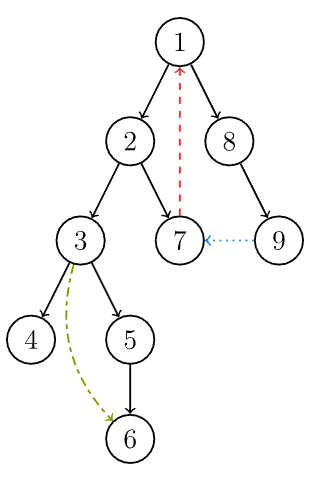
\includegraphics[width=0.3\textwidth,center]{../photo/dfstree}
\indent一颗DFS生成树包含四种类型的边,\textbf{树边,返祖边,横叉边,前向边}。\\
\indent定义DFN(u)为节点u搜索的次序编号(时间戳),Low(u)为u或u的子树能够追溯到的最早的\textbf{栈中}节点的次序号。
\subsection{强连通分量}
\begin{lstlisting}[language=C++]
void tarjan(int u)
{
    dfn[u]=low[u]=++tim;
    atack.push(u);inst[u]=1;
    for(int i=head[u];~i;i=r[i].nex)
    {
        int v=r[i].b;
        if(dfn[v]==0)
        {
            tarjan(v);low[u]=min(low[u],low[v]);
        }
        else if(inst[v]==1) low[u]=min(low[u],dfn[v]);
    }
    if(dfn[u]==low[u])
    {
        numb++;int q;
        do
        {
            q=atack.top();inst[q]=0;atack.pop();
            bl[q]=numb;nums[numb]++;
        }while(q!=u);
    }
}
\end{lstlisting}
将多个强连通分量加边联通为一个强连通分量,最少需要$\max (num_{ru=0},num_{chu=0})$条边,只有一个强连通分量需要特判。
\subsection{双连通分量}
只要删去桥还能够保持联通,就是边双连通。
\begin{lstlisting}[language=C++,title=边双连通分量]
void tarjan(int u,int f)//f是路线编号
{
    atack.push(u);
    dfn[u]=low[u]=++tim;
    for(int i=head[u];~i;i=r[i].nex)
    {
        int v=r[i].b;
        if(!dfn[v])
        {
            tarjan(v,i);low[u]=min(low[u],low[v]);
        }
        else if(i!=(f^1)) low[u]=min(low[u],dfn[v]);
    }
    if(dfn[u]==low[u])
    {
        numb++;int t;
        do
        {
            t=atack.top();atack.pop();
            bl[t]=numb;nums[numb]++;
        }while(t!=u);
    }
}
\end{lstlisting}
只要删去割点还能保持联通,就是点双连通,但是要注意,一个割点可能同时属于多个点双连通分量。\textbf{注意特判自环!!!!}
\begin{lstlisting}[language=C++,title=点双连通分量]
void tarjan(int u,int root)//有没有fa其实无所谓
{
    dfn[u]=low[u]=++tim;
    atack.push(u);
    if(u==root && head[u]==-1)//特判孤立点
    {
        dcc[++numb].push_back(u);return;
    }
    int child=0;
    for(int i=head[u];~i;i=r[i].nex)
    {
        int v=r[i].b;
        if(!dfn[v])
        {
            tarjan(v,root);
            low[u]=min(low[u],low[v]);
            if(dfn[u]==low[v])
            {
                child++;
                if(u!=root||child>1) isgd[u]=true;
                numb++;
                int y;
                do{
                    y=atack.top();atack.pop();
                    dcc[numb].push_back(y);
                }while(y!=v);
                dcc[numb].push_back(u);
            }
        }
        else low[u]=min(low[u],dfn[v]);
    }
}
\end{lstlisting}
\subsection{割点和桥}
将某点及其连边删去,图无法继续连通。
\begin{lstlisting}[language=C++,title=割点]
void tarjan(int u,int root)
{
    dfn[u]=low[u]=++tim;
    int child=0;
    for(int i=head[u];~i;i=r[i].nex)
    {
        int v=r[i].b;
        if(!dfn[v])
        {
            tarjan(v,root);
            low[u]=min(low[u],low[v]);
            if(low[v]==dfn[u])
            {
                child++;
                if(u!=root || child>1)	isgd[u]=1;
            }
        }
        else
        low[u]=min(low[u],dfn[v]);
    }
}
\end{lstlisting}
删去图中的某个边,图不再连通,无向图只包含树边和非树边,没有非树边覆盖的树边就是桥。
\begin{lstlisting}[language=C++,title=桥]
void tarjan(int u,int f)//f是路线编号
{
    dfn[u]=low[u]=++tim;
    for(int i=head[u];~i;i=r[i].nex)
    {
        int v=r[i].b;
        if(!dfn[v])
        {
            tarjan(v,i);
            low[u]=min(low[u],low[v]);
            if(dfn[u]<low[v])//和割点的区别
            {
                isbri[i]=isbri[i^1]=1;
            }
        }
        else if(i!=(f^1))
        low[u]=min(low[u],dfn[v]);
    }
}
\end{lstlisting}
一棵树上有$n$个度数为$1$的点,最少连接$(n+1)/2$条边即可变为双连通分量。
\subsection{圆方树}
\indent众所周知,树(或森林)有很好的性质,并且容易通过很多常见数据结构维护。\\
\indent而一般图则没有那么好的性质,所幸有时我们可以把一般图上的某些问题转化到树上考虑。\\
\indent顾名思义,圆方树即有圆点有方点的树。\\
\indent在一张无向图中,将图中原有的点视为圆点,将图中的点双连通分量视为一个方点,将方点对应的圆点用菊花图的连接方式连接起来。就会形成一颗(或多颗)圆方树(森林)。\\
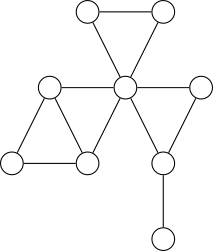
\includegraphics[width=0.33\textwidth]{../photo/yfs1.png}
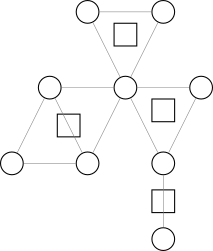
\includegraphics[width=0.33\textwidth]{../photo/yfs2.png}
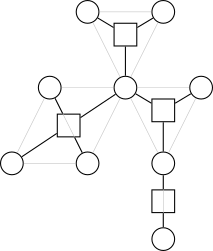
\includegraphics[width=0.33\textwidth]{../photo/yfs3.png}
\noindent\textbf{技巧:}\\
\indent1.对圆方树上圆点权值初始化为$-1$,方点权值初始化为度数大小。任意两圆点在树上路径权值之和即为原无向图两点路径途经点集的数量和。
\indent2.无向图任意两点间的割点数,等价于圆方树上两点树上路径上的圆点数量。
\begin{lstlisting}
void tarjan(int u)
{
    dfn[u]=low[u]=++tim;
    stk.push(u);
    for(int i=head[u];~i;i=r[i].nex)
    {
        int v=r[i].b;
        if(!dfn[v])
        {
            tarjan(v);low[u]=min(low[u],low[v]);
            if(low[v]==dfn[u])
            {
                idx++;int x;
                do
                {
                    x=stk.top();stk.pop();
                    rst[idx].push_back(x);
                    rst[x].push_back(idx);
                }while(x!=v);
                rst[u].push_back(idx);
                rst[idx].push_back(u);
            }
        }
        else low[u]=min(low[u],dfn[v]);
    }
}
\end{lstlisting}
\section{仙人掌}
仙人掌图(cactus)是一种无向连通图,它的每条边最多只能出现在一个简单回路里面。从直观上说,可以把仙人掌图理解为允许存在回路的树。如果一个图不包含\textbf{偶数环}那么这个图一定是仙人掌。\\
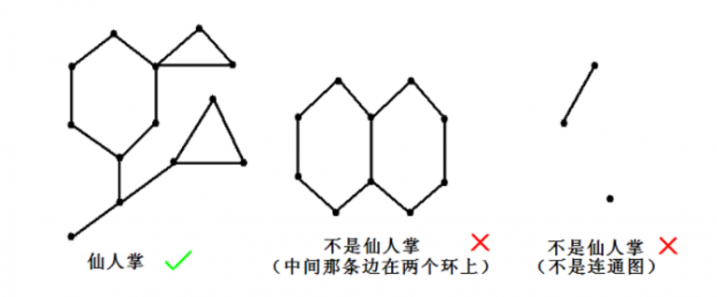
\includegraphics[width=0.5\textwidth,center]{../photo/xrz.png}
\subsubsection{仙人掌圆方树}
上述圆方树在某种意义上被认为是广义圆方树,即适用于一般无向图的圆方树。对于仙人掌,我们对其使用狭义圆方树。两种圆方树一个明显的区别就是,一个只有两个点的点双联通分量要不要建方点。因此除了广义圆方树上仅有的圆方边,在此类圆方树中还包含圆圆边,但两种圆方树中都不存在方方边。\\
\indent仙人掌图本质上是一个树上开花(环)的树,因此我们对其做边双连通分量,对于树边(桥),继续用原图上的边对其连接(圆圆边),如果遇到了环,对环上节点依次与其方点连接。建好的树即为仙人掌圆方树。\\
\subsubsection{仙人掌上最短路}
对于圆圆边,边权为原边边权,圆方边的边权为$0$,方圆边的边权为原图上圆点到方点父亲的最短路。\\
\indent建好树后,记$dis(x)$为$x$点到树根的距离,对于$u$到$v$的最短路,若其LCA为圆点,最短路即$dis(u)+dis(v)-2*dis(LCA)$。若为方点,找出LCA的两个儿子$A,B$,分别为$u,v$的祖先,此时最短路即$dis(A,B)+dis(u,A)+dis(v,B)$。其中$dis(A,B)$可以通过预处理环长计算。
\begin{lstlisting}[language=c++]
#include<bits/stdc++.h>
using namespace std;
typedef long long ll;
const int maxn=20005;
int n,m,q,f[maxn][16],head[maxn],dep[maxn],num,dfn[maxn],low[maxn],tim,idx;
int sum[maxn],len[maxn],fa[maxn],dis[maxn],A,B;
struct road{int b,c,nex;}r[2000005];
void add(int a,int b,int c){r[num].b=b;r[num].c=c;r[num].nex=head[a];head[a]=num++;}
stack<int>stk;
vector<pair<int,int>>rst[maxn];
void build_tree(int u,int v,int val)
{
    int pre=val,x=v;
    while(x!=fa[u])
    {
        sum[x]=pre;pre+=len[x];x=fa[x];
    }
    sum[++idx]=sum[u];
    x=v;rst[u].push_back({idx,0});
    while(x!=u)
    {
        int mn=min(sum[idx]-sum[x],sum[x]);
        rst[idx].push_back({x,mn});x=fa[x];
    }
}
void tarjan(int u,int from)
{
    dfn[u]=low[u]=++tim;
    stk.push(u);
    for(int i=head[u];~i;i=r[i].nex)
    {
        int v=r[i].b;
        if(!dfn[v])
        {
            len[v]=r[i].c;fa[v]=u;
            tarjan(v,i);
            low[u]=min(low[u],low[v]);
        }
        else if(i!=(from^1)) low[u]=min(low[u],dfn[v]);
        if(low[v]>dfn[u]) //桥=圆圆边
        {
            rst[u].push_back({v,r[i].c});
        }
    }
    for(int i=head[u];~i;i=r[i].nex)
    {
        int v=r[i].b;
        if(fa[v]==u||dfn[v]<=dfn[u]) continue;
        build_tree(u,v,r[i].c);
    }
}
void dfs(int u,int fa)
{
    f[u][0]=fa;dep[u]=dep[fa]+1;
    for(int i=1;i<=15;i++) f[u][i]=f[f[u][i-1]][i-1];
    for(auto [nex,w]:rst[u])
    {
        dis[nex]=dis[u]+w;
        dfs(nex,u);
    }
}
int lca(int a,int b)
{
    if(dep[a]<dep[b]) swap(a,b);
    for(int i=15;i>=0;i--)
    {
        if(dep[f[a][i]]>=dep[b]) a=f[a][i];
    }
    if(a==b) return a;
    for(int i=15;i>=0;i--)
    {
        if(f[a][i]!=f[b][i]) a=f[a][i],b=f[b][i]; 
    }
    A=a,B=b;
    return f[a][0];
}
int main()
{
    memset(head,-1,sizeof(head));
    scanf("%d%d%d",&n,&m,&q);idx=n;
    for(int i=1;i<=m;i++)
    {
        int u,v,w;scanf("%d%d%d",&u,&v,&w);
        add(u,v,w);add(v,u,w);
    }
    tarjan(1,-1);
    dfs(1,0);
    while(q--)
    {
        int a,b;scanf("%d%d",&a,&b);
        int LCA=lca(a,b);
        if(LCA<=n) printf("%d\n",dis[a]+dis[b]-2*dis[LCA]);
        else printf("%d\n",dis[a]+dis[b]-dis[A]-dis[B]+min(abs(sum[A]-sum[B]),sum[LCA]-abs(sum[A]-sum[B])));
    }
}
\end{lstlisting}


\section{2-SAT}
\indent个人认为2-SAT跟强连通的关系有点像差分约束跟最短路的关系。\\
\indent\textbf{k-SAT问题}:有$n$个$bool$类型的事件,有$m$种约束,每种约束都有$k$个事件的关系。找出一种符合约束的$n$个事件的取值。(NP完全问题)\\
\indent将$n$个事件拆分为$2*n$个点,分别代表$0,1$两种情况。对于所有的约束,我们根据题意建立有向图。若在有向图中有$(a\Rightarrow b)$,则意为选择了$a$一定要同时选择$b$才可以满足约束条件。\\
\indent根据题意建好图后,应首先判断事件约束是否合法。对其进行\textbf{强连通分量缩点},若$a,b$在同一个强连通分量内,则意味着$a,b$绑定在了一起,必须同时选取才能满足约束。这种情况下,如果某个事件的$0,1$情况在同一个强连通分量下,该事件就又要为$1$又要为$0$,显然这是矛盾的。\\
\indent在判断完上述情况后,就一定存在满足约束要求的合法方案。优先选择强连通分量标号较小的情况,因为在Tarjan结束后的出栈顺序决定了缩点后DAG的拓扑序。
\begin{center}
\begin{tabular}{|c|c|}
\hline 
原式 & 构图\\
\hline 
$a\lor b=1$ & $(\neg a\Rightarrow b)\land(\neg b\Rightarrow a)$\\
\hline 
$a \& b=1$ & $(\neg a\Rightarrow a)\land(\neg b\Rightarrow b)$ \\
\hline 
$a \& b=0$ & $(a\Rightarrow \neg b)\land(b\Rightarrow \neg a)$ \\
\hline
$a \mid b=1$ & $(\neg a\Rightarrow b)\land(\neg b\Rightarrow a)$  \\
\hline
$a \mid b=0$ & $(a\Rightarrow \neg a)\land(b\Rightarrow \neg b)$\\
\hline
$a\oplus b=1$ & $(a\Rightarrow \neg b)\land(\neg a\Rightarrow b)\land(b \Rightarrow \neg a)\land(\neg b\Rightarrow a)$\\
\hline
$\quad a\oplus b=0 \quad$ & $\quad (a\Rightarrow b)\land(\neg a\Rightarrow \neg b)\land(b \Rightarrow a)\land(\neg b\Rightarrow \neg a)\quad$\\
\hline
\end{tabular}    
\end{center}

\begin{lstlisting}[language=c++]
for(int i=1;i<=n;i++)
{
    if(bl[i]==bl[i+n]){puts("IMPOSSIBLE");return 0;}
}
puts("POSSIBLE");
for(int i=1;i<=n;i++)
{
    if(bl[i]<bl[i+n]) printf("1 ");
    else printf("0 ");
}
\end{lstlisting}

\section{图的匹配}
\begin{itemize}
    \item 最大匹配: 匹配数最多的匹配。
    \item 完美匹配: 所有点都属于匹配,同时也符合最大匹配。
    \item 近完美匹配: 发生在图的点数为奇数,刚好只有一个点不在匹配中。
\end{itemize}
\subsubsection{增广路定理}
\indent交错路:始于非匹配点且由匹配边与非匹配边交错而成。\\
\indent增广路:是始于非匹配点且终于非匹配点的交错路。\\
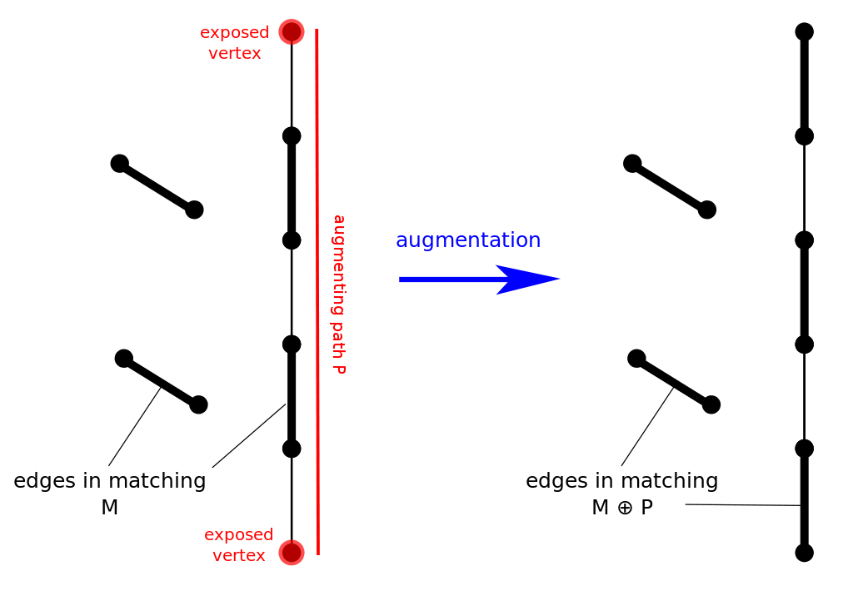
\includegraphics[width=0.5\textwidth,center]{../photo/Berge's lemma}\\
\indent增广路上非匹配边比匹配边数量多一,如果将匹配边改为未匹配边,反之亦然,则匹配大小会增加一且依然是交错路。
\subsection{二分图}
\subsubsection{染色法判断二分图}
\begin{lstlisting}[language=c++]
bool dfs(int u,int color)
{
    col[u]=color;
    for(int i=head[u];~i;i=r[i].nex)
    {
        int next=r[i].b;
        if(col[next]==0)
        {
            if(!dfs(next,3-color)) return false;
        }
        else
        {
            if(col[next]==color) return false;
        }
    }
    return true;
}
\end{lstlisting}
\subsubsection{二分图完美匹配}
设$G=<V_1,V_2,E>$为二分图,$|V_1|\leq|V_2|$,$M$为$G$中一个最大匹配,且$M=|V_1|$,则称$M$为$V_1$到$V_2$的完美匹配。
\subsubsection{霍尔定理}
对于一个二分图,如果对于左边任意子集$S$,其对应边连接了一个右边的边集$T$,都有$|S|<=|T|$,那么这个二分图有完美匹配(充要)。
\subsection{二分图最大匹配}
\subsubsection{匈牙利算法}
\begin{lstlisting}[language=c++,title=邻接矩阵$O(n^3)$]
bool match(int x)
{
    for(int i=1;i<=n2;i++)
    {
        if(side[x][i]&&!vis[i])
        {
            vis[i]=1; //将i加入增广路上
            if(!mat[i]||match(mat[i])) 
            {
                mat[i]=x;return true;
            }
        }
    }
    return false;
}
int Hungarian()
{
    int ans=0;
    for(int i=1;i<=n1;i++)
    {
        memset(vis,0,sizeof(vis));
        if(match(i)) ans++;
    }
    return ans;
}
\end{lstlisting}
\begin{itemize}
    \item 换用邻接表,可将时间优化至$O(nm)$,使用网络流建图跑dinic,时间复杂度$O(m\sqrt n)$。
    \item 若同侧匹配,记得反向记录mat,且第一次开始递归的节点$x$标记vis[x]=1。
\end{itemize}
\subsubsection{二分图最小点覆盖(König 定理)}
\indent最小点覆盖:选最少的点,满足每条边至少有一个端点被选。\\
\indent二分图中,最小点覆盖$=$最大匹配。
\subsubsection{二分图最大独立集}
\indent最大独立集:选最多的点,满足两两之间没有边相连。\\
\indent因为在最小点覆盖中,任意一条边都被至少选了一个顶点,所以对于其点集的补集,任意一条边都被至多选了一个顶点,所以不存在边连接两个点集中的点,且该点集最大。因此二分图中,最大独立集$=$总点$-$最小点覆盖。
\subsection{二分图最大权匹配}
\subsubsection{KM算法}
\indent本质上是匈牙利算法$+$贪心。\\
\indent将两个集合中点数比较少的补点,使得两边点数相同,再将不存在的边权重设为$0$,这种情况下,问题就转换成求\textbf{最大权完美匹配问题},从而能应用KM算法求解。\\
\indent\textbf{可行顶标:}给每个节点$i$分配一个权值$l(i)$,对于所有边$w(u,v)$满足$w(u,v)\leq l(u)+l(v)$。\\
\indent\textbf{相等子图:}在一组可行顶标下原图的生成子图,包含所有点但只包含满足$w(u,v)\leq l(u)+l(v)$的边$w(u,v)$。\\
\indent我们的目标就是透过不断的调整可行顶标,使得相等子图是完美匹配。\\
\indent在一开始,我们让图中左侧的点的相等子图都贪心的连向最大的匹配边,初始化顶标$lx(i)=\max_{1\leq j\leq n}\{w(i,j)\},ly(i)=0$。\\
\indent然后我们开始在图上增广,找到增广路就增广,否则,会得到一个交错树。\\
\indent令$S$,$T$表示二分图左边右边在交错树中的点$S'$,$T'$表示不在交错树中的点。\\
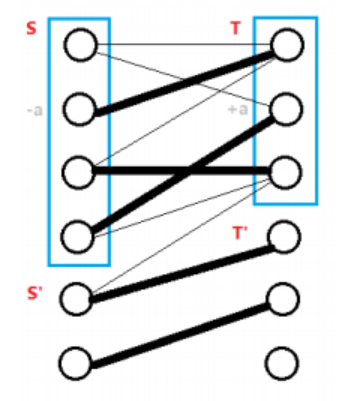
\includegraphics[width=0.3\textwidth,center]{../photo/km}\\
\indent此时无法继续修改,这时我们只能修改一些顶标使得相等子图发生变化从而可以继续匹配下去,这就意味着$S$中的某点必须做出让步,去匹配一些权值稍微低一点的边。我们找出$S\sim T'$中权值最小的边,权值$a=\min\{lx(u)+ly(v)-w(u,v)| u\in S,v\in T'\}$,使得损失尽可能降低。\\
\indent使$S$中的顶标$-a$,$T$中的顶标$+a$,可以发现:$S\sim T$边依然在相等子图中。$S' \sim T'$没有变化。$S\sim T'$的$lx+ly$减少,有可能加入相等子图。$S'\sim T$的边不可能加入相等子图。\\
\indent相等子图发生了变化,观察是否可以匹配,否则重复上述过程。由于原图一定存在完美匹配,所以最多$n$次一定可以找到增广路。\\
\indent一开始枚举$n$个点找增广路,为了找增广路需要延伸$n$次交错树,每次延伸需要$n$次维护,共$O(n^3)$。
\begin{lstlisting}[language=c++,escapeinside=``]
bool check(int v)
{
    visy[v]=1;
    if(maty[v]!=-1)
    {
        q.push(maty[v]);visx[maty[v]]=1;
        return false;
    }
    while(v!=-1){maty[v]=pre[v];swap(v,matx[pre[v]]);}
    return true;
}
void bfs(int x)
{
    while(!q.empty()) q.pop();
    q.push(x);visx[x]=1;
    while(1)
    {
        while(!q.empty())//`使用BFS进行匹配`
        {
            int u=q.front();q.pop();
            for(int v=1;v<=n;v++)
            {
                if(visy[v]) continue;
                int delta=lx[u]+ly[v]-side[u][v];
                if(slack[v]<delta) continue;
                pre[v]=u; //`delta=0意为改边属于相等子图`
                if(delta) slack[v]=delta;
                else if(check(v)) return;
            }
        }
        int mn=1e9;//匹配失败
        for(int i=1;i<=n;i++) if(!visy[i]) mn=min(mn,slack[i]);
        for(int i=1;i<=n;i++)
        {
            if(visx[i]) lx[i]-=mn;
            if(visy[i]) ly[i]+=mn;
            else slack[i]-=mn;
        }
        for(int i=1;i<=n;i++)
        {
            if (!visy[i]&&slack[i]==0&&check(i)) return;
        }
    }
}
void km()
{
    memset(lx,0,sizeof(lx));
    memset(ly,0,sizeof(ly));
    memset(matx,-1,sizeof(matx));
    memset(maty,-1,sizeof(maty));
    for(int i=1;i<=n;i++)
    {
        for(int j=1;j<=n;j++) lx[i]=max(lx[i],side[i][j]);
    }
    for(int i=1;i<=n;i++)
    {
        memset(visx,0,sizeof(visx));
        memset(visy,0,sizeof(visy));
        memset(slack,0x3f,sizeof(slack));
        bfs(i);//`slack[i]的值为右边第i个点和左边的点的顶标的最大值`
    }
    int ans=0;
    for(int i=1;i<=n;i++) ans+=side[i][matx[i]];
    printf("%d\n",ans);
    for(int i=1;i<=n;i++) printf("%d ",maty[i]);
}
\end{lstlisting}
\subsubsection{转化为费用流模型}
\indent在图中新增一个源点和一个汇点。\\
\indent从源点向二分图的每个左部点连一条流量为$1$,费用为$0$的边,从二分图的每个右部点向汇点连一条流量为$1$,费用为$0$的边。\\
\indent接下来对于二分图中每一条连接左部点$u$和右部$v$,边权为$w$的边,则连一条从$u$到$v$,流量为$1$,费用为$w$的边。\\
\indent求这个网络的\textbf{最大费用最大流}即可得到答案。
\subsection{一般图最大匹配}
\subsubsection{带花树}
\indent一般图匹配和二分图匹配不同的是,图可能存在奇环。时间复杂度$O(n^3)$\\
\begin{lstlisting}[language=c++,escapeinside=``]
int find(int x){return fa[x]==x?x:fa[x]=find(fa[x]);}
int LCA(int u,int v)
{
    ++tim;u=find(u);v=find(v);
    while(dfn[u]!=tim)//`u,v轮流上跳,直到跳到环顶`
    {
        dfn[u]=tim;
        u=find(pre[mat[u]]);
        if(v) swap(u,v);
    }
    return u;
}
void Blossom(int x,int y,int w)
{//对奇环进行缩花,同时将图上所有白点涂黑,向环外增广
    while(find(x)!=w)
    {
        pre[x]=y,y=mat[x];
        if(vis[y]==2) vis[y]=1,q.push(y);
        if(find(x)==x) fa[x]=w;
        if(find(y)==y) fa[y]=w;
        x=pre[y];
    }
}
int bfs(int x)
{
    for(int i=1;i<=n;i++) fa[i]=i,vis[i]=pre[i]=0;
    while(!q.empty()) q.pop(); q.push(x);vis[x]=1;
    while(!q.empty())
    {
        int u=q.front();q.pop();
        for(int i=head[u];~i;i=r[i].nex)
        {
            int v=r[i].b;
            //`u,v在同一朵花中或v是白色(偶环)`
            if(find(u)==find(v) || vis[v]==2) continue;
            if(!vis[v]) //`如果v尚未染色`
            {
                vis[v]=2;pre[v]=u;
                if(!mat[v])//增广成功
                {
                    for(int j=v,last;j;j=last) 
                    last=mat[pre[j]],mat[j]=pre[j],mat[pre[j]]=j;
                    return 1;
                }
                vis[mat[v]]=1;q.push(mat[v]);
            }
            else //`如果v是黑色,出现奇环,开花`
            {
                int w=LCA(v,u);//第一次进入奇环的黑点
                Blossom(u,v,w);Blossom(v,u,w);
            }
        }
    }
    return 0;
}
void match()
{
    int ans=0;
    for(int i=1;i<=n;i++) if(!mat[i] && bfs(i)) ans++;
    printf("%d\n",ans);
    for(int i=1;i<=n;i++) printf("%d ",mat[i]);
    puts("");
}
\end{lstlisting}
\section{网络流}
\subsection{最大流}
\subsubsection{EK算法}
EK算法就是BFS找增广路,然后对其进行增广,时间复杂度$O(nm^2)$。
\begin{lstlisting}[language=c++]
int bfs(int s,int t)
{
    memset(vis,0,sizeof(vis));
    queue<int>q;q.push(s);
    vis[s]=1;incf[s]=1e18;
    while(!q.empty())
    {
        int u=q.front();q.pop();
        for(int i=head[u];~i;i=r[i].nex)
        {
            int v=r[i].b;
            if(vis[v] || r[i].c==0) continue;
            q.push(v);vis[v]=1;pre[v]=i^1;
            incf[v]=min(incf[u],r[i].c);
            if(v==t) return 1;
        }
    }
    return 0;
}
int EK(int s,int t)
{
    int p=t;
    while(p!=s)
    {
        r[pre[p]].c+=incf[t];
        r[pre[p]^1].c-=incf[t];
        p=r[pre[p]].b;
    }
    return incf[t];
}
\end{lstlisting}
\subsubsection{Dinic算法}
\indent Dinic算法的过程是这样的:每次增广前,我们先用BFS来将图分层。设源点的层数为$0$,那么一个点的层数便是它离源点的最近距离。\\
\indent 然后使用DFS对流量进行增广,每次找增广路的时候,都只找比当前点层数多$1$的点进行增广(这样就可以确保我们找到的增广路是最短的),时间复杂度$O(n^2m)$。\\
\indent多路增广优化:每次找到一条增广路的时候,如果残余流量没有用完怎么办呢?我们可以利用残余部分流量,再找出一条增广路。这样就可以在一次DFS中找出多条增广路,大大提高了算法的效率。\\
\indent当前弧优化:如果一条边已经被增广过,那么它就没有可能被增广第二次。那么,我们下一次进行增广的时候,就可以不必再走那些已经被增广过的边。
\begin{lstlisting}[language=c++]
int make_level()
{
    memset(depth,-1,sizeof(depth));
    queue<int>q;q.push(s);
    depth[s]=1;now[s]=head[s];//当前弧优化
    while(!q.empty())
    {	
        int u=q.front();q.pop();
        for(int i=head[u];~i;i=r[i].nex)
        {
            int v=r[i].b;
            if(depth[v]!=-1 || r[i].c<=0) continue;
            now[v]=head[v];
            depth[v]=depth[u]+1;
            q.push(v);
        }
    }
    return depth[t]!=-1;
}
int dinic(int u,int flow)
{
    if(u==t) return flow;
    int sum=0;
    for(int i=now[u];~i;i=r[i].nex)//多路增广
    {
        now[u]=i;
        int v=r[i].b;
        if(depth[v]!=depth[u]+1 || r[i].c<=0) continue;
        int use=dinic(v,min(flow-sum,r[i].c));
        if(use)
        {
            r[i].c-=use;r[i^1].c+=use;
            sum+=use;
        }
        if(sum==flow) return flow;
    }
    if(sum==0) depth[u]=-1;
    return sum;
}
\end{lstlisting}
\subsubsection{ISAP}
\indent在Dinic算法中,我们每次求完增广路后都要跑BFS来分层,有没有更高效的方法呢?ISAP是一种只需要一次BFS就可以不断增广的写法。\\
\indent和Dinic算法一样,我们还是先跑BFS对图上的点进行分层,不过与Dinic略有不同的是,我们选择在反图上,从$t$点向$s$点进行BFS。\\
\indent设$i$号点的层为$d_i$,当我们结束在$i$号点的增广过程后,我们遍历残量网络上$i$的所有出边,找到层最小的出点$j$,随后令$d_i=d_j+1$。特别地,若残量网络上$i$无出边,则$d_i=n$。时间复杂度$O(n^3)$\\
\indent GAP优化:记录每一层的点的数量,若某层为空,即出现了断层,直接结束。
\begin{lstlisting}[language=c++,escapeinside=``]
void make_level()
{
    queue<int>q;q.push(t);
    depth[t]=1;gap[1]++;
    while(!q.empty())
    {
        int u=q.front();q.pop();
        for(int i=head[u];~i;i=r[i].nex)
        {
            int v=r[i].b;
            if(depth[v]) continue;
            depth[v]=depth[u]+1;
            gap[depth[v]]++;
            q.push(v);
        }
    }
}
ll dfs(ll u,ll flow)
{
    if(u==t) return flow;
    ll sum=0;
    for(int i=head[u];~i;i=r[i].nex)
    {
        ll v=r[i].b;
        if(depth[v]+1!=depth[u] || r[i].c==0) continue;
        ll use=dfs(v,min(flow-sum,r[i].c));
        if(use)
        {
            r[i].c-=use;
            r[i^1].c+=use;
            sum+=use;
        }	
        if(sum==flow) return flow;
    }
    gap[depth[u]]--;
    if(gap[depth[u]==0]) depth[s]=n+1;//GAP优化
    depth[u]++;gap[depth[u]]++;
    return sum;
}
void ISAP()
{
    make_level();
    while(depth[s]<=n) 
    {
        ans+=dfs(s,1e18);
    }
}
\end{lstlisting}
\subsubsection{HPLL}
时间复杂度$O(n^2\sqrt m)$
\begin{lstlisting}[language=c++]
#include<bits/stdc++.h>
using namespace std;
const int N = 1200, M = 120000, INF = 0x3f3f3f3f;
int n, m, s, t;
struct qxx {int nex, t, v;};
qxx e[M * 2 + 1];
int h[N + 1], cnt = 1;
void add_path(int f, int t, int v) { 
    e[++cnt] = (qxx){h[f], t, v}, h[f] = cnt; }
void add_flow(int f, int t, int v) {
    add_path(f, t, v);
    add_path(t, f, 0);
}
int ht[N + 1], ex[N + 1],
    gap[N];  // 高度; 超额流; gap 优化 gap[i] 为高度为 i 的节点的数量
stack<int> B[N];  // 桶 B[i] 中记录所有 ht[v]==i 的v
int level = 0;    // 溢出节点的最高高度
int push(int u) {      // 尽可能通过能够推送的边推送超额流
    bool init = u == s;  // 是否在初始化
    for (int i = h[u]; i; i = e[i].nex) {
        const int &v = e[i].t, &w = e[i].v;
        if (!w || init == false && ht[u] != ht[v] + 1)  // 初始化时不考虑高度差为1
        continue;
        int k = init ? w : min(w, ex[u]);
        // 取到剩余容量和超额流的最小值,初始化时可以使源的溢出量为负数。
        if(v!=s && v!=t && !ex[v]) B[ht[v]].push(v),level= max(level, ht[v]);
        ex[u] -= k, ex[v] += k, e[i].v -= k, e[i ^ 1].v += k;  // push
        if (!ex[u]) return 0;  // 如果已经推送完就返回
    }
    return 1;
}
void relabel(int u) {  // 重贴标签(高度)
    ht[u] = INF;
    for (int i = h[u]; i; i = e[i].nex)
        if (e[i].v) ht[u] = min(ht[u], ht[e[i].t]);
    if (++ht[u] < n) {  // 只处理高度小于 n 的节点
        B[ht[u]].push(u);
        level = max(level, ht[u]);
        ++gap[ht[u]];  // 新的高度,更新 gap
    }
}
bool bfs_init() {
    memset(ht, 0x3f, sizeof(ht));
    queue<int> q;
    q.push(t), ht[t] = 0;
    while (q.size()) {  // 反向 BFS, 遇到没有访问过的结点就入队
        int u = q.front();
        q.pop();
        for (int i = h[u]; i; i = e[i].nex) {
        const int &v = e[i].t;
        if (e[i ^ 1].v && ht[v] > ht[u] + 1) ht[v] = ht[u] + 1, q.push(v);
        }
    }
    return ht[s] != INF;  // 如果图不连通,返回 0
}
// 选出当前高度最大的节点之一, 如果已经没有溢出节点返回 0
    int select() {
    while (B[level].size() == 0 && level > -1) level--;
    return level == -1 ? 0 : B[level].top();
}
int hlpp() {                  // 返回最大流
    if (!bfs_init()) return 0;  // 图不连通
    memset(gap, 0, sizeof(gap));
    for (int i = 1; i <= n; i++)
        if (ht[i] != INF) gap[ht[i]]++;  // 初始化 gap
    ht[s] = n;
    push(s);  // 初始化预流
    int u;
    while ((u = select())) {
        B[level].pop();
        if (push(u)) {  // 仍然溢出
        if (!--gap[ht[u]])
            for (int i = 1; i <= n; i++)
            if (i != s && i != t && ht[i] > ht[u] && ht[i] < n + 1)
                ht[i] = n + 1;  // 这里重贴成 n+1 的节点都不是溢出节点
        relabel(u);
        }
    }
    return ex[t];
}
int main() {
    scanf("%d%d%d%d", &n, &m, &s, &t);
    for (int i = 1, u, v, w; i <= m; i++) {
        scanf("%d%d%d", &u, &v, &w);
        add_flow(u, v, w);
    }
    printf("%d", hlpp());
    return 0;
}
\end{lstlisting}
\subsection{最小割}
对于一个网络流图$G=(V,E)$,其割的定义为一种点的划分方式:将所有的点划分为$S$和$T=V-S$两个集合,其中源点$s\in S$,汇点$t \in T$。
\subsubsection{方案}
我们可以通过从源点$s$开始DFS,每次走残量大于$0$的边,找到所有$S$点集内的点。
\begin{lstlisting}[language=c++]
void dfs(int u)
{
    vis[u]=1;
    for(int i=head[u];~i;i=r[i].nex)
    {
        int v=r[i].b;
        if(!vis[v]&&r[i].c) dfs(v);
    }
}
\end{lstlisting}
\subsubsection{割边数量}
如果需要在最小割的前提下最小化割边数量,那么先求出最小割,把没有满流的边容量改成$inf$,满流的边容量改成$1$,重新跑一遍最小割就可求出最小割边数量;如果没有最小割的前提,直接把所有边的容量设成$1$,求一遍最小割就好了。
\subsubsection{问题模型1:二者选其一}
\indent有$n$个物品和两个集合$A,B$,如果一个物品没有放入$A$集合会花费$a_i$,没有放入$B$集合会花费$b_i$;还有若干个形如$u_i,v_i,w_i$限制条件,表示如果$u_i$和$v_i$同时不在一个集合会花费$w_i$。每个物品必须且只能属于一个集合,求最小的代价。\\
\indent我们对于每个集合设置源点$s$和汇点$t$,第$i$个点由$s$连一条容量为$a_i$的边、向$t$连一条容量为$b_i$的边。对于限制条件$u,v,w$,我们在$u,v$之间连容量为$w$的双向边。\\
\indent最小割就是最小花费。
\subsubsection{问题模型2:最大权闭合图}
\indent最大权值闭合图,即给定一张有向图,每个点都有一个权值(可以为正或负或$0$),你需要选择一个权值和最大的子图,使得子图中每个点的后继都在子图中。\\
\indent做法:建立超级源点$s$和超级汇点$t$,若节点$u$权值为正,则$s$向$u$连一条有向边,边权即为该点点权;若节点$u$权值为负,则由$u$向$t$连一条有向边,边权即为该点点权的相反数。原图上所有边权改为$inf$。跑网络最大流,将所有正权值之和减去最大流,即为答案。\\
\indent此外,该图应该是一个拓扑图,如果无法满足则应该先拓扑排序找出合法的边。\\
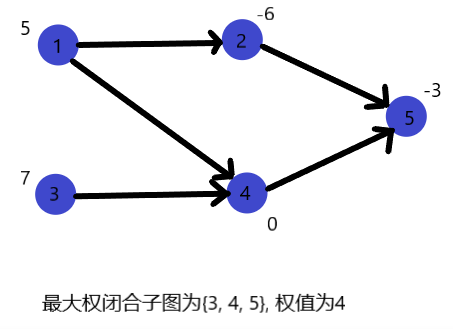
\includegraphics[width=0.4\textwidth,center]{../photo/zxg1}
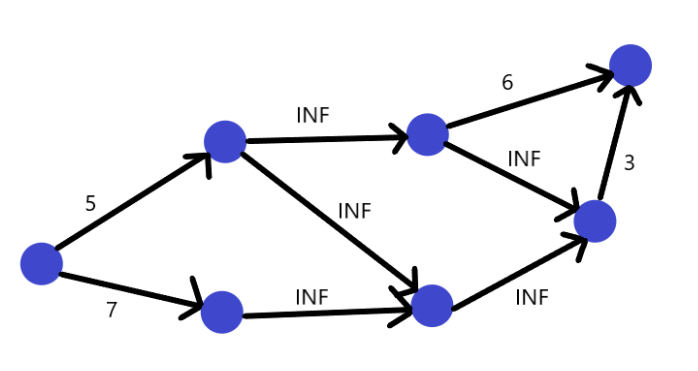
\includegraphics[width=0.5\textwidth,center]{../photo/zxg2}\\
\indent判断一条边是否被割,应该通过最后一次增广后,depth是否为$-1$来判断。
\subsection{费用流}
只需将EK算法或Dinic算法中找增广路的过程,替换为用最短路/最长路算法寻找单位费用最小的增广路即可。
\begin{lstlisting}[language=c++,title=最小费用最大流]
bool spfa()
{
    for(int i=1;i<=n;i++)
    {
        pre[i]=-1;vis[i]=0;dis[i]=inf;
    }
    incf[s]=inf;
    queue<int>q;q.push(s);
    dis[s]=0;vis[s]=1;
    while(!q.empty())
    {
        int u=q.front();q.pop();
        vis[u]=0;
        for(int i=head[u];~i;i=r[i].nex)
        {
            int v=r[i].b;
            if(r[i].c && dis[v]>dis[u]+r[i].d)
            {
                dis[v]=dis[u]+r[i].d;
                incf[v]=min(incf[u],r[i].c);
                pre[v]=i;
                if(vis[v]==0)
                {
                    vis[v]=1;
                    q.push(v);
                }
            }
        }
    }
    if(pre[t]==-1) return false;
    return true;
}
void MCMF()
{
    while(spfa())
    {
        int x=t;
        maxflow+=incf[t];
        mincost+=incf[t]*dis[t];
        while(x!=s)
        {
            r[pre[x]].c-=incf[t];
            r[1^pre[x]].c+=incf[t];
            x=r[1^pre[x]].b;
        }
    }
}
\end{lstlisting}
\subsection{上下界网络流}
\subsubsection{无源汇上下界可行流}
\indent给定无源汇流量网络$G$。询问是否存在一种标定每条边流量的方式,使得每条边流量满足上下界同时每一个点流量平衡(循环环流)。一个满足流量平衡的点意味着该点的流入流量等于流出流量。\\
\indent首先每条边的流量应该大于其下界流量。假设每条边当前都只流出了其下界,用下界流量记录各点的流量平衡状态。在这个条件的基础上建立一个新图,新图每条边的流量为:流量上界$-$流量下界,也就是图上剩余的流量值。\\
\indent建立虚拟源汇点$S',T'$。若点$u$流出量大于流入量,差值为$M$,我们就从$S'$出发向$u$连接一条值为$M$的附加边。若点$u$流出量小于流入量,差值为$M$,我们就从$u$出发向$T'$连接一条值为$M$的附加边。\\
\indent如果附加边满流,说明这一个点的流量平衡条件可以满足,否则这个点的流量平衡条件不满足。在建图完毕之后跑$S'$到$T'$的最大流,若$S'$连出去的边全部满流,则存在可行流,否则不存在。
\subsubsection{有源汇上下界可行流}
\indent给定有源汇流量网络$G$。询问是否存在一种标定每条边流量的方式,使得每条边流量满足上下界同时除了源点和汇点每一个点流量平衡。\\
\indent假设源点为$S$,汇点为$T$。则我们可以加入一条$T$到$S$的上界为$\infty$,下界为$0$的边转化为无源汇上下界可行流问题。若有解,则$S$到$T$的可行流流量等于$T$到$S$的附加边的流量。
\subsubsection{有源汇上下界最大流}
\indent首先,先判断是否存在有源汇上下界可行流。如果找不到解就可以直接结束。\\
\indent记计算出来的上下界可行流为$flow1$。否则,我们删去图上所有的附加边,在残量网络上算出$S$到$T$计算出最大流$flow2$。有源汇上下界最大流$=flow1+flow2$。
\begin{lstlisting}[language=C++,title=有源汇上下界最大流]
#include<bits/stdc++.h>
#define inf 0x3f3f3f3f
using namespace std;
int n,m,in[205],out[205],depth[205],now[205],head[205],s,t,num,low[200005];
struct road{int b,c,nex;}r[200005];
void add(int a,int b,int c){
    r[num].b=b;r[num].c=c;r[num].nex=head[a];head[a]=num++;}
int make_level()
{
    memset(depth,-1,sizeof(depth));
    queue<int>q;q.push(s);
    depth[s]=1;now[s]=head[s];
    while(!q.empty())
    {	
        int u=q.front();q.pop();
        for(int i=head[u];~i;i=r[i].nex)
        {
            int v=r[i].b;
            if(depth[v]!=-1 || r[i].c<=0) continue;
            now[v]=head[v];
            depth[v]=depth[u]+1;
            q.push(v);
        }
    }
    return depth[t]!=-1;
}
int dinic(int u,int flow)
{
    if(u==t) return flow;
    int sum=0;
    for(int i=now[u];~i;i=r[i].nex)
    {
        now[u]=i;
        int v=r[i].b;
        if(depth[v]!=depth[u]+1 || r[i].c<=0) continue;
        int use=dinic(v,min(flow-sum,r[i].c));
        if(use)
        {
            r[i].c-=use;r[i^1].c+=use;
            sum+=use;
        }
        if(sum==flow) return flow;
    }
    if(sum==0) depth[u]=-1;
    return sum;
}
int main()
{
    memset(head,-1,sizeof(head));
    scanf("%d%d%d%d",&n,&m,&s,&t);
    for(int i=1;i<=m;i++)
    {
        int a,b,u;scanf("%d%d%d%d",&a,&b,&low[i],&u);
        add(a,b,u-low[i]);add(b,a,0);
        out[a]+=low[i];in[b]+=low[i];//记录各点的流量进出状况
    }
    int s1=n+1,t1=s1+1;
    int sum=0,st=num;
    for(int i=1;i<=n;i++)
    {
        if(in[i]==out[i]) continue;//建立附加边
        if(in[i]>out[i]) add(s1,i,in[i]-out[i]),add(i,s1,0);
        else add(i,t1,out[i]-in[i]),add(t1,i,0),sum+=abs(in[i]-out[i]);
    }
    add(t,s,inf);add(s,t,0);//建立附加边
    int ans=0;
    swap(s,s1);swap(t,t1);
    while(make_level()) ans+=dinic(s,1e9);
    if(ans==sum)//存在可行流
    {
        int flow1=r[num-1].c;
        for(int i=st;i<num;i++) r[i].c=0; //删除图上所有的附加边
        swap(s,s1);swap(t,t1);
        while(make_level()) flow1+=dinic(s,inf); //flow1+flow2
        printf("%d\n",flow1);
    }
    else//不存在可行流
        puts("please go home to sleep");
}
\end{lstlisting}
\subsubsection{有源汇上下界最小流}
\indent首先,先判断是否存在有源汇上下界可行流。如果找不到解就可以直接结束。\\
\indent记计算出来的上下界可行流为$flow1$。否则,我们删去图上所有的附加边,在残量网络上算出$T$到$S$计算出最大流$flow2$。意为将多余的无用流量退还回去,有源汇上下界最大流$=flow1-flow2$。
\section{Stoer-Wagner算法}
\indent Stoer-Wagner算法是一种解决无向正权图上的\textbf{全局最小割}问题的算法。算法复杂度$O(nm+n^2\log|n|)$一般可近似看作$O(n^3)$。\\
\noindent\textbf{算法过程:}\\
\indent1.在图$G$中任意指定两点$s,t$,并且以这两点作为源汇点求出最小割,更新当前答案。\\
\indent2.将$t$合并入$s$变为同一点。合并过程:删除$s,t$之间的连边,对于$G/{s,t}$中任意一点$k$,删除$t,k$,并将其边权$d(t,k)$加到$d(s,k)$上。\\
\indent3.输出所有最小割的最小值。\\
\indent若选择的割边会将两点$s,t$分为两个连通块,则该割边的大小即以$s,t$为源汇的最小割。否则,$s,t$将绑定在一起,共享所有的边。因此,处理完一对$s,t$之间的最小割后,就只有它们处于同一连通块的情况了,也就是做完一对以后就合并一对点,如是进行次$n-1$即合并成一个点,算法完成。\\
\noindent\textbf{最小割求法:}\\
\indent假设进行若干次合并以后,当前图$G'=(V',E')$,我们构造一个集合$A$,初始时令$A=\varnothing$。\\
\indent我们每次将$G'$中所有点中,满足$i\notin A$,且权值函数$w(i)$最大的节点加入集合$A$,直到$|A|=|V'|$。\\
\indent其中$w(i)=\displaystyle\sum_{j\in A}d(i,j)$。\\
\indent令$ord(i)$表示第$i$个加入$A$的点,令$s$为$ord(|V'-1|)$,$t$为$ord(|V'|)$,则此时的$w(t)$就是$s$到$t$的最小割。
\begin{lstlisting}[language=c++,escapeinside=``]
int contract(int x) 
{
    memset(vis,0,sizeof(vis));
    memset(w,0,sizeof(w));
    w[0]=-1;
    for(int i=1;i<=n-x+1;i++) 
    {
        int mx=0;
        for (int j=1;j<=n;j++) 
        {   //`dap[j]=1表示j点已经与其他点合并`
            if(!dap[j]&&!vis[j]&&w[j]>w[mx]) mx=j;
        }
        vis[mx]=1,ord[i]=mx; //`第i个加入集合A的点是ord[i]`
        for(int j=1;j<=n;j++) 
        {
            if(!dap[j]&&!vis[j]) w[j]+=side[mx][j]; //`更新维护w函数`
        }
    }
    s=ord[n-x],t=ord[n-x+1]; //`这样的s和t的最小割一定是w[t]`
    return w[t];
}
int Stoer_Wagner() 
{
    int res=INF;
    for (int i=1;i<n;i++) 
    {
        res=min(res,contract(i));
        dap[t]=1; //`将t与s合并`
        for (int j=1;j<=n;j++) 
        {
            side[s][j]+=side[t][j];
            side[j][s]+=side[j][t];
        }
    }
    return res;
}
\end{lstlisting}
\section{特殊的图}
\subsection{竞赛图}
竞赛图也叫有向完全图。每对顶点之间都有一条边相连的有向图称为竞赛图。
\begin{itemize}
    \item 竞赛图没有自环,没有二元环;若竞赛图存在环,则一定存在三元环。(如果存在一个环大于三元,那么一定存在另一个三元的小环。)
    \item 任意竞赛图都有哈密顿路径(经过每个点一次的路径,不要求回到出发点)。
    \item 图存在哈密顿回路的充要条件是强联通。
\end{itemize}
\subsubsection{兰道定理}
兰道定理是用来判定竞赛图的定理。将一个竞赛图的每一个点的出度从小到大排序后得到长度为$n$的序列称为竞赛图的比分序列$s={s_1\leq s_2 \leq \cdots \leq s_n}$是合法的比分序列当且仅当:
$$
\forall 1\leq k \leq n,\sum_{i=1}^{k} s_i \ge\binom{k}{2} 
$$
且$k=n$时一定相等。
\subsection{平面图}
\indent如果可以将一个图画在二维平面上,可以存在一种画法使任意两条边都不相交,该图就是平面图。\\
\subsubsection{如何判断一个图是不是平面图?}
\noindent拓扑学欧拉公式:对于一个连通平面图$G=(V,E,F),|V|-|E|+|F|=2$则该图为平面图,其中$|V|,|E|,|F|$分别为点数,边数,和形成的面数(面内不应该有其余的边,且最外面的无限大的区域也算一个面)。\\
\noindent证明:对于一棵树,一定是平面图,且满足$|V|-|E|+|F|=2$,此后,每增加一条边,都会多一条边和一个面。平面图边数和点数的关系:$m \leq 3*n-6$。
\subsection{对偶图}
对偶图是与平面图相伴的一种图。将平面图中的每个面都变为一个点,将各个面割开的边变为新的边,权值不变,连接在新的点上。对偶图的对偶图是原图。\\
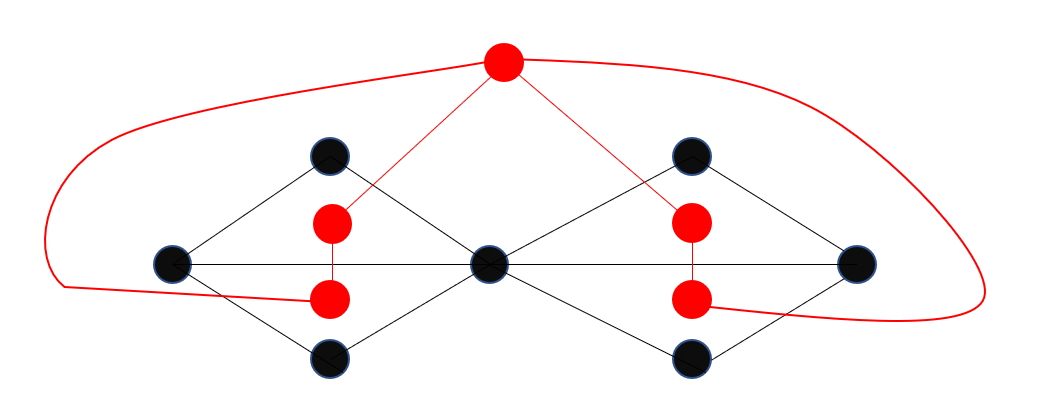
\includegraphics[width=0.5\textwidth,center]{../photo/duiou.png}
\subsubsection{平面图的最小割等于其对偶图的最短路}
对于一个$s-t$平面图,我们对其进行如下改造:首先连接$s-t$得到一个附加面,求该图的对偶图$G$,令附加面对应的点为$s$,无界面对应的点为$t$,然后对图$G$进行连边,此时$s-t$最短路就是最小割。\\
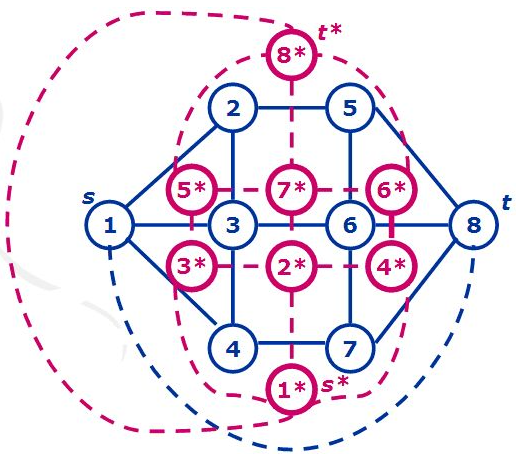
\includegraphics[width=0.5\textwidth,center]{../photo/duiou2.png}
\section{最小环}
给出一个图,问其中的有$n$个节点构成的边权和最小的环$(n\ge3)$是多大。二元化较为特殊,处理方法也比较简单。
\subsubsection{Dijkstra}
设$u$和$v$之间有一条边长为$w$的边,$dis(u,v)$表示删除$u$和$v$之间的连边之后,两点之间的最短路。那么图中的最小环是$dis(u,v)+w$。时间复杂度$O(m(n+m)\log n)$。
\subsubsection{floyd}
\begin{lstlisting}[language=c++,escapeinside=``]
int val[maxn+1][maxn+1]; //原图的邻接矩阵
int floyd(int &n) 
{
    int dis[maxn+1][maxn+1]; //最短路矩阵
    for(int i=1;i<=n;++i)
        for(int j=1;j<=n;++j) dis[i][j]=val[i][j]; //初始化最短路矩阵
    int ans=inf;
    for(int k=1;k<=n;++k) 
    {
        for(int i=1;i<k;++i)
            for(int j=1;j<i;++j)
            ans=min(ans,dis[i][j]+val[i][k]+val[k][j]); //更新答案
        for(int i=1;i<=n;++i)
            for(int j=1;j<=n;++j)
            dis[i][j]=min(dis[i][j],dis[i][k]+dis[k][j]);
    }
    return ans;
}
\end{lstlisting}
\ifx\allfiles\undefined
\end{document}
\fi




    \chapter{数据结构}
    \ifx\allfiles\undefined
\documentclass[a4paper]{book}
\usepackage{ctex}
\usepackage{graphicx} %插入图片
\usepackage{amsmath}
\usepackage{amsthm}
\usepackage{lmodern}
\usepackage{float}
\usepackage[export]{adjustbox}
\usepackage{listings,xcolor} %代码块
\usepackage{txfonts}
\usepackage{xcolor}
\usepackage{listings}
\lstset{
    breaklines,                                 % 自动将长的代码行换行排版
    extendedchars=false,                        % 解决代码跨页时,章节标题,页眉等汉字不显示的问题
    backgroundcolor=\color[rgb]{0.96,0.96,0.96},% 背景颜色
    keywordstyle=\color{blue}\bfseries,         % 关键字颜色
    identifierstyle=\color{black},              % 普通标识符颜色
    commentstyle=\color[rgb]{0,0.6,0},          % 注释颜色
    stringstyle=\color[rgb]{0.58,0,0.82},       % 字符串颜色
    showstringspaces=false,                     % 不显示字符串内的空格
    numbers=left,                               % 显示行号
    numberstyle=\small\ttfamily,                % 设置数字字体
    basicstyle=\small\ttfamily,                 % 设置基本字体
    captionpos=t,                               % title在上方(在bottom即为b)
    frame=single,                               % 设置代码框形式
    rulecolor=\color[rgb]{0.8,0.8,0.8},         % 设置代码框颜色
}  
   

\begin{document}
\fi
\section{并查集}
\subsubsection{带权并查集}
\begin{lstlisting}[language=c++]
int find(int x)
{
    if(x!=fa[x])
    {
        int t=fa[x];fa[x]=find(fa[x]);
        v[x]=(v[x]+v[t])%2;
    }
    return fa[x];
}
void lianjie(int x,int y,int s)
{
    int px=find(x),py=find(y);
    fa[px]=py;
    v[px]=(-v[x]+v[y]+s+2)%2;
}
\end{lstlisting}
\section{单调栈}
定义函数$f(i)$代表数列中第$i$个元素之后第一个大于$a_i$的元素的下标。若不存在,则$f(i)=0$。
\begin{lstlisting}[language=c++]
for(int i=n;i>=1;i--)
{
    while(!s.empty() && a[s.top()]<=a[i]) s.pop();
    if(s.size()==0) f[i]=0;
    else f[i]=s.top();
    s.push(i);
}
\end{lstlisting}
\section{单调队列}
有一个长为$n$的序列$a$,以及一个大小为$k$的窗口。现在这个从左边开始向右滑动,每次滑动一个单位,求出每次滑动后窗口中的最大值。
\begin{lstlisting}[language=c++]
deque<int>q;
for(int i=1;i<=n;i++)
{
    if(!q.empty() && q.front()<=i-k) q.pop_front();
    while(!q.empty() && a[q.back()]<=a[i]) q.pop_back();
    q.push_back(i);
    if(i>=k) printf("%lld\n",a[q.front()]);
}
\end{lstlisting}
\section{ST表}
\begin{lstlisting}[language=c++]
void ST()
{
    for(int j=1;j<21;j++)
    {
        for(int i=1;i+(1<<(j-1))<=n;i++)
        {
            f[i][j]=max(f[i][j-1],f[i+(1<<(j-1))][j-1]);
        }
    }
}
int query(int l,int r)
{
    int k=log2(r-l+1);
    return max(f[l][k],f[r-(1<<k)+1][k]);
}
\end{lstlisting}
\section{树状数组}
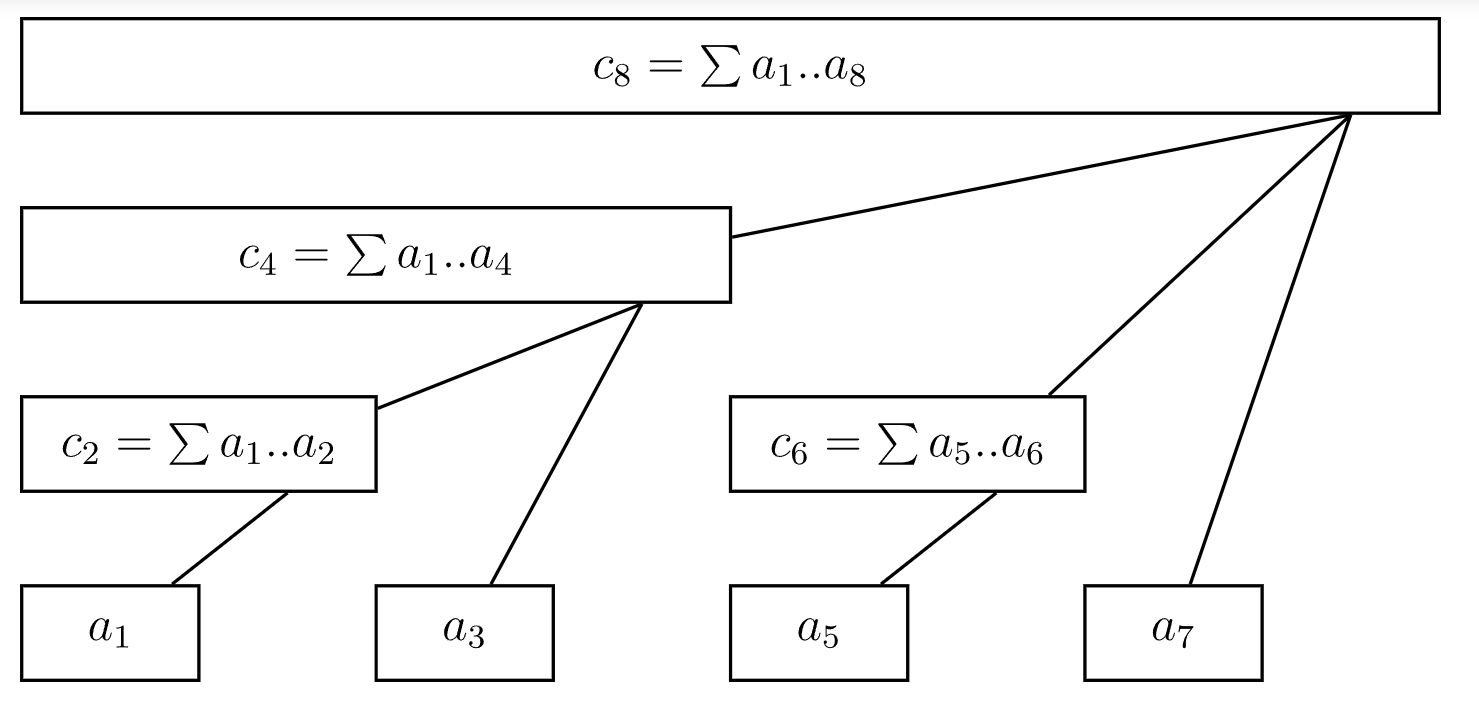
\includegraphics[width=0.7\textwidth,center]{../photo/fenwick}
\subsubsection{单点修改}
\begin{lstlisting}[language=c++]
void update(int num,int x)
{
    for(int i=num;i<=n;i+=lowbit(i)) tre[i]+=x;
}
ll query(int num)
{
    ll sum=0;
    for(int i=num;i>0;i-=lowbit(i)) sum+=tre[i];
    return sum;
}
\end{lstlisting}
\subsubsection{区间修改}
维护序列$a$的差分数组$b$,此时我们对$a$的一个前缀$r$求和,即$\sum_{i=1}^{r}a_i$,由差分数组定义得$a_i=\sum_{j=1}^{i}b_j$。
$$
\begin{aligned}
    &\sum_{i=1}^{r}a_i\\
    =&\sum_{i=1}^{r}\sum_{j=1}^{i}b_j\\
    =&\sum_{i=1}^{r}b_i\times(r-i+1)\\
    =&\sum_{i=1}^{r}b_i\times(r+1)-\sum_{i=1}^{r}b_i\times i
\end{aligned}
$$
区间和可以用两个前缀和相减得到,因此只需要用两个树状数组分别维护$\sum b_i$和$\sum i\times b_i$,就能实现区间求和。
\begin{lstlisting}[language=c++,escapeinside=``]
//`tre1表示b的前缀和,tre2表示b*i的前缀和,b表示原数组的差分数组`
void update(int num,int x)
{ 
    for(int i=num;i<=n;i+=lowbit(i)) tre1[i]+=x,tre2[i]+=num*x;
}
void update(int l,int r,int x)
{
    update(l,x);update(r+1,-x);
}
ll query(ll tre[],int x)
{
    ll sum=0;
    for(int i=x;i>0;i-=lowbit(i)) sum+=tre[i];
    return sum;
}
ll query(int x)
{
    return query(tre1,x)*(x+1)-query(tre2,x);
}
\end{lstlisting}
\subsubsection{查询第$k$小/大元素}
\indent在此处只讨论第$k$小,第$k$大问题可以通过简单计算转化为第$k$小问题。\\
\indent找到最大的$x$满足$\sum_{i=1}^x a_i<k$,那么$x+1$就是我们的答案。在树状数组中,节点是根据$2$的幂划分的,每次可以扩大$2$的幂的长度。令$sum$表示当前的$x$所代表的前缀和,有如下算法找到最大的:
\begin{enumerate}
    \item 求出$depth=\left\lfloor\log_2n\right\rfloor$
    \item 计算$t=\displaystyle\sum_{i=x+1}^{x+2^{depth}} a_i$
    \item 如果$sum+t<k$,则此时扩展成功,将$2^{depth}$累加到$x$上;否则扩展失败,对$x$不进行操作
    \item 将$depth$减$1$,回到步骤$2$,直至$depth$为$0$
\end{enumerate}
\begin{lstlisting}[language=c++,escapeinside=``]
// 权值树状数组查询第k小
int kth(int k) 
{
    int cnt=0,ret=0;
    for(int i=log2(n);~i;--i) //`i与上文depth含义相同`
    {      
        ret+=1<<i; //尝试扩展
        if(ret>=n||cnt+tre[ret]>=k) //`如果扩展失败`
            ret-=1<<i;
        else cnt+=tre[ret]; //`扩展成功后,要更新之前求和的值`
    }
    return ret+1;
}
\end{lstlisting}
\section{线段树}
\subsection{单点修改}
\begin{lstlisting}[language=c++]
struct tree
{
    int l,r,sum;
    int mid(){return (l+r)/2;}
}tre[maxn<<2];
void pushup(int num)
{
    tre[num].sum=tre[2*num].sum+tre[2*num+1].sum;
}
void build(int num,int l,int r)
{
    tre[num].l=l,tre[num].r=r;
    if(l==r)
    {
        tre[num].sum=a[l];return;
    }
    int mid=tre[num].mid();
    build(2*num,l,mid);build(2*num+1,mid+1,r);
    pushup(num);
}
int query(int num,int l,int r)
{
    if(tre[num].l==l && tre[num].r==r)
    return tre[num].sum;
    int mid=tre[num].mid();
    if(l>mid) return query(2*num+1,l,r);
    else if(r<=mid) return query(2*num,l,r);
    else return(query(2*num,l,mid)+query(2*num+1,mid+1,r));
}
void add(int num,int n,int k)
{
    if(tre[num].l==tre[num].r) tre[num].sum+=k;return;
    int mid=tre[num].mid();
    if(n<=mid) add(2*num,n,k);
    else add(2*num+1,n,k);
    pushup(num);
}
\end{lstlisting}
\subsection{区间修改}
\begin{lstlisting}[language=c++]
struct tree
{
    ll l,r,sum,lazy;
    ll mid(){return (l+r)/2;}
}tre[4*maxn];
void build(ll num,ll l,ll r)
{
    tre[num].l=l;tre[num].r=r;
    tre[num].lazy=0;
    if(l==r)
    {
        tre[num].sum=a[l];
        return;
    }
    ll mid=tre[num].mid();
    build(2*num,l,mid);build(2*num+1,mid+1,r);
    tre[num].sum=tre[2*num].sum+tre[2*num+1].sum;
}
void pushdown(ll num)
{
    tre[2*num].sum+=(tre[2*num].r-tre[2*num].l+1)*tre[num].lazy;
    tre[2*num+1].sum+=(tre[2*num+1].r-tre[2*num+1].l+1)*tre[num].lazy;
    tre[2*num].lazy+=tre[num].lazy;
    tre[2*num+1].lazy+=tre[num].lazy;
    tre[num].lazy=0;
}
ll query(ll num,ll l,ll r)
{
    if(tre[num].l==l && tre[num].r==r) return tre[num].sum;
    pushdown(num);
    ll mid=tre[num].mid();
    if(l>mid) return query(2*num+1,l,r);
    else if(r<=mid) return query(2*num,l,r);
    else return query(2*num,l,mid)+query(2*num+1,mid+1,r);
}
void update(ll num,ll l,ll r,ll k)
{
    if(tre[num].l==l && tre[num].r==r)
    {
        tre[num].sum+=(tre[num].r-tre[num].l+1)*k;
        tre[num].lazy+=k;
        return;
    }
    pushdown(num);
    ll mid=tre[num].mid();
    if(l>mid) update(2*num+1,l,r,k);
    else if(r<=mid) update(2*num,l,r,k);
    else
    {
        update(2*num,l,mid,k);update(2*num+1,mid+1,r,k);
    }
    tre[num].sum=tre[2*num].sum+tre[2*num+1].sum;
}
\end{lstlisting}
\section{势能线段树}
\begin{lstlisting}[language=c++,title=区间进行lowbit操作]
struct tree
{
    ll l,r,sum,lazy,flag;
    ll mid(){return (l+r)/2;}
}tre[4*maxn];
int check(int num)
{
    int cnt=0;
    for(int i=32;i>=0;i--) if(tre[num].sum>>i&1) cnt++;
    if(cnt==1) 
    {
        tre[num].sum%=mod;
        return 1;
    }
    return 0;
}
void pushdown(ll num)
{
    int lazy=tre[num].lazy;
    if(lazy==0) return;
    tre[2*num].sum=(tre[2*num].sum*p[lazy])%mod;
    tre[2*num+1].sum=(tre[2*num+1].sum*p[lazy])%mod;
    tre[2*num].lazy+=tre[num].lazy;
    tre[2*num+1].lazy+=tre[num].lazy;
    tre[num].lazy=0;
}
void pushup(int num)
{
    tre[num].sum=(tre[2*num].sum+tre[2*num+1].sum)%mod;
    tre[num].flag=tre[2*num].flag&tre[2*num+1].flag;
}
void build(ll num,ll l,ll r)
{
    tre[num].l=l;tre[num].r=r;
    tre[num].lazy=0;tre[num].sum=0;tre[num].flag=0;
    if(l==r)
    {
        tre[num].sum=a[l];tre[num].flag=check(num);
        return;
    }
    ll mid=tre[num].mid();
    build(2*num,l,mid);build(2*num+1,mid+1,r);
    pushup(num);
}
ll query(ll num,ll l,ll r)
{
    if(tre[num].l==l && tre[num].r==r)
    {
        return tre[num].sum%mod;
    }
    pushdown(num);
    ll mid=tre[num].mid();
    if(l>mid) return query(2*num+1,l,r);
    else if(r<=mid) return query(2*num,l,r);
    else return (query(2*num,l,mid)+query(2*num+1,mid+1,r))%mod;
}
void update(ll num,ll l,ll r)
{
    ll mid=tre[num].mid();
    if(tre[num].l==l && tre[num].r==r)
    {
        if(tre[num].flag)
        {
            tre[num].sum=(tre[num].sum*2)%mod;tre[num].lazy++;
        }
        else
        {
            if(l==r)
            {
                tre[num].sum=lowbit(tre[num].sum)+tre[num].sum;
                tre[num].flag=check(num);
            }
            else
            {
                update(2*num,l,mid);update(2*num+1,mid+1,r);
                pushup(num);
            }

        }
        return;
    }
    pushdown(num);
    if(l>mid) update(2*num+1,l,r);
    else if(r<=mid) update(2*num,l,r);
    else
    {
        update(2*num,l,mid);update(2*num+1,mid+1,r);
    }
    pushup(num);
}
\end{lstlisting}
\section{主席树}
\subsubsection{区间第$k$大}
\begin{lstlisting}[language=c++]
int build(int l,int r)
{
    int pos=++cnt;
    lch[pos]=0,rch[pos]=0,sum[pos]=0;
    if(l<r)
    {
        int mid=l+r>>1;
        lch[pos]=build(l,mid);
        rch[pos]=build(mid+1,r);
    }
    return pos;
}
int update(int pre,int l,int r,ll x)
{
    int pos=++cnt;
    lch[pos]=lch[pre],rch[pos]=rch[pre],sum[pos]=sum[pre];
    if(l<r)
    {
        int mid=l+r>>1;
        if(x<=mid) lch[pos]=update(lch[pre],l,mid,x);
        else rch[pos]=update(rch[pre],mid+1,r,x);
        sum[pos]=sum[lch[pos]]+sum[rch[pos]];
    }
    else sum[pos]++;
    return pos;
}
int query(int x,int y,int l,int r,int k)
{
    if(l==r) return l;
    int mid=l+r>>1;
    int nn=sum[lch[y]]-sum[lch[x]];
    if(nn<k) return query(rch[x],rch[y],mid+1,r,k-nn);
    else return query(lch[x],lch[y],l,mid,k);
}
\end{lstlisting}
\section{树上差分}
\subsection{点差分}
$$
\begin{aligned}
    &d_s \leftarrow d_s+1\\
    &d_{lca} \leftarrow d_{lca}-1\\
    &d_t \leftarrow d_t+1 \\
    &d_{f(lca)} \leftarrow d_{f(lca)}-1
\end{aligned}
$$
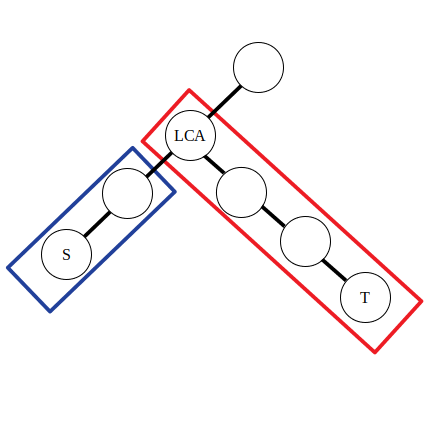
\includegraphics[width=0.4\textwidth,center]{../photo/prefix_sum1.png}
\subsection{边差分}
$$
\begin{aligned}
    &d_s \leftarrow d_s+1\\
    &d_t \leftarrow d_t+1 \\
    &d_{lca} \leftarrow d_{lca}-2\\
\end{aligned}
$$
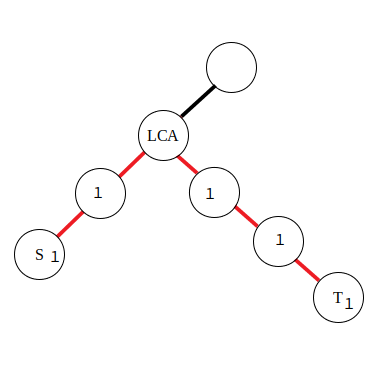
\includegraphics[width=0.4\textwidth,center]{../photo/prefix_sum2.png}
\section{树链剖分}
\subsubsection{重链剖分}
\begin{lstlisting}[language=c++]
void dfs1(int u,int fa)
{
    sz[u]=1;big[u]=-1;dep[u]=dep[fa]+1;par[u]=fa;
    for(auto nex:v[u])
    {
        if(nex==fa) continue;
        dfs1(nex,u);sz[u]+=sz[nex];
        if(big[u]==-1||sz[big[u]]<sz[nex]) big[u]=nex;
    }
}
void dfs2(int u,int fa,int t)
{
    top[u]=t;dfn[u]=++tim;rk[tim]=u;
    if(big[u]==-1) return;
    dfs2(big[u],u,t);
    for(auto nex:v[u])
    {
        if(nex==fa||nex==big[u]) continue;
        dfs2(nex,u,nex);
    }
}
struct SegTree
{
    struct tree
    {
        int l,r;ll sum;
        int mid(){return l+r>>1;}
    }tre[maxn<<2];
    void pushup(int num)
    {
        tre[num].sum=tre[2*num].sum+tre[2*num+1].sum;
    }
    void build(int num,int l,int r)
    {
        tre[num].l=l;tre[num].r=r;
        if(l==r)
        {
            tre[num].sum=a[rk[l]];return;
        }
        int mid=tre[num].mid();
        build(2*num,l,mid);build(2*num+1,mid+1,r);
        pushup(num);
    }
    ll query_sum(int num,int l,int r)
    {
        if(tre[num].l==l&&tre[num].r==r)
        {
            return tre[num].sum;
        }
        int mid=tre[num].mid();
        if(l>mid) return query_sum(2*num+1,l,r);
        else if(r<=mid) return query_sum(2*num,l,r);
        else return query_sum(2*num,l,mid)+query_sum(2*num+1,mid+1,r);
    }
    void update(int num,int pos,int x)
    {
        if(tre[num].l==tre[num].r)
        {
            tre[num].sum=x;return;
        }
        int mid=tre[num].mid();
        if(pos<=mid) update(2*num,pos,x);
        else update(2*num+1,pos,x);
        pushup(num);
    }
}st;
ll query_sum(int x,int y)
{
    ll res=0,fx=top[x],fy=top[y];
    while(fx!=fy)
    {
        if(dep[fx]>=dep[fy]) res+=st.query_sum(1,dfn[fx],dfn[x]),x=par[fx];
        else res+=st.query_sum(1,dfn[fy],dfn[y]),y=par[fy];
        fx=top[x],fy=top[y];
    }
    if(dfn[x]<dfn[y]) res+=st.query_sum(1,dfn[x],dfn[y]);
    else res+=st.query_sum(1,dfn[y],dfn[x]);
    return res;
}
\end{lstlisting}
\section{莫队}
\begin{lstlisting}[language=c++,title=区间不同种类元素个数]
#include<bits/stdc++.h> 
using namespace std;
int n,m,a[50005],vis[1000005],len;
struct node{int l,r,id;}q[200005];
int ans[200005],res=0;
bool cmp(node a,node b)
{
	int al=a.l/len,bl=b.l/len;
	if(al!=bl) return al<bl;
	return a.r<b.r;
}
void add(int num)
{
	vis[a[num]]++;
	if(vis[a[num]]==1) res++;
}
void del(int num)
{
	vis[a[num]]--;
	if(vis[a[num]]==0) res--;
} 
int main()
{
	scanf("%d",&n);len=sqrt(n);
	for(int i=1;i<=n;i++) scanf("%d",&a[i]);
	scanf("%d",&m);
	for(int i=1;i<=m;i++)
	{
		scanf("%d%d",&q[i].l,&q[i].r);q[i].id=i;
	}
	sort(q+1,q+1+m,cmp);
	int l=1,r=0;
	for(int i=1;i<=m;i++)
	{
		int id=q[i].id,ll=q[i].l,rr=q[i].r;
		while(r<rr) add(++r);
		while(r>rr) del(r--);
		while(l<ll) del(l++);
		while(l>ll) add(--l);
		ans[id]=res;
	}
	for(int i=1;i<=m;i++) printf("%d\n",ans[i]);
}
\end{lstlisting}
\ifx\allfiles\undefined
\end{document}
\fi



    \chapter{字符串}
    \ifx\allfiles\undefined
\documentclass[a4paper]{book}
\usepackage{ctex}
\usepackage{graphicx} %插入图片
\usepackage{amsmath,amsthm}
\usepackage{lmodern}
\usepackage{float}
\usepackage[export]{adjustbox}
\usepackage{listings,xcolor} %代码块
\usepackage{xcolor}
\usepackage{listings}
\lstset{
    breaklines,                                 % 自动将长的代码行换行排版
    extendedchars=false,                        % 解决代码跨页时,章节标题,页眉等汉字不显示的问题
    backgroundcolor=\color[rgb]{0.96,0.96,0.96},% 背景颜色
    keywordstyle=\color{blue}\bfseries,         % 关键字颜色
    identifierstyle=\color{black},              % 普通标识符颜色
    commentstyle=\color[rgb]{0,0.6,0},          % 注释颜色
    stringstyle=\color[rgb]{0.58,0,0.82},       % 字符串颜色
    showstringspaces=false,                     % 不显示字符串内的空格
    numbers=left,                               % 显示行号
    numberstyle=\small\ttfamily,                % 设置数字字体
    basicstyle=\small\ttfamily,                 % 设置基本字体
    captionpos=t,                               % title在上方(在bottom即为b)
    frame=single,                               % 设置代码框形式
    rulecolor=\color[rgb]{0.8,0.8,0.8},         % 设置代码框颜色
}  
   

\begin{document}
\fi
\section{字符串哈希}
\begin{lstlisting}[language=c++]
struct Hash
{
    ll mod,base,h[maxn],p[maxn],n;
    void make_hash()
    {
        p[0]=1;
        for(int i=1;i<=n;i++)
        {
            h[i]=((h[i-1]%mod*base%mod)%mod+s[i])%mod;
            p[i]=(p[i-1]*base)%mod;
        }
    }
    ll get_hash(ll l,ll r)
    {
        return (h[r]-(h[l-1]%mod*p[r-l+1]%mod)%mod+mod)%mod;
    }
}h;
\end{lstlisting}
\subsubsection{允许$k$次失配的字符串匹配}
\indent模式串$t$与主串$s$进行匹配时,若不同的位置不大于$k$个,则认为匹配成功。\\
\indent哈希$+$二分。枚举所有可能匹配的子串,假设现在枚举的子串为$s'$,通过哈希$+$二分可以快速找到$s'$与$t$第一个不同的位置。之后将$s'$与$t$在这个失配位置及之前的部分删除掉,继续查找下一个失配位置。这样的过程最多发生$k$次。时间复杂度$O(m+kn\log m)$。\\
\subsubsection{最长回文子串}
\indent记$R_i$表示以$i$作为结尾的最长回文的长度,那么答案就是$\max_{i=1}^{n}R_i$。考虑到$R_{i-1}\leq R_i+2$,因此我们只需要暴力从$R_{i-1}+2$开始递减,直到找到第一个回文即可。记变量$z$表示当前枚举的$R_i$,初始时为$0$,则$z$在每次$i$增大的时候都会增大$2$,之后每次暴力循环都会减少$1$,故暴力循环最多发生$2n$次,总的时间复杂度为$O(n)$。\\
\subsubsection{最长公共子字符串}
\indent给定$m$个总长不超过$n$的非空字符串,查找所有字符串的最长公共子字符串。\\
\indent二分最长公共子字符串的长度。假设现在的长度为$k$,check(k) 的逻辑为我们将所有所有字符串的长度为$k$的子串分别进行哈希,将哈希值放入$n$个哈希表中存储。之后求交集即可。时间复杂度$O(n\log\frac{n}{m})$。
\section{字典树}
\begin{lstlisting}[language=c++]
void insert(char s[])
{
    int p=0,l=strlen(s);
    for(int i=0;i<l;i++)
    {
        int u=s[i]-'a';
        if(!trie[p][u]) trie[p][u]=++cnt;
        p=trie[p][u];		
    }
    son[p]++;
}
int find(char s[])
{
    int p=0,l=strlen(s);
    for(int i=0;i<l;i++)
    {
        int u=s[i]-'a';
        if(!trie[p][u]) return -1;
        p=trie[p][u];
    }
    return son[p];
}
\end{lstlisting}
\subsubsection{维护异或和}
\indent使用Trie维护多个数字的异或和可以实现:“插入”,“删除”,“全局加一”的功能。与使用Trie维护异或极值不同的是,如果要维护异或和,需要按值从低位到高位建立Trie。\\
\subsubsection{插入\&删除}
\indent如果要维护异或和,我们只需要知道某一位上$0$和$1$个数的奇偶性即可,也就是对于数字$1$来说,当且仅当这一位上数字$1$的个数为奇数时,这一位上的数字才是$1$。\\
\indent num[u]是指字典树上到达u点的数量。xorv[u]指以u为根的子树维护的异或和,xorv[root]即维护的异或和。
\begin{lstlisting}[language=c++,escapeinside=``]
void maintain(int p)
{
    num[p]=xorv[p]=0;
    if(trie[p][0]) 
        num[p]+=num[trie[p][0]],xorv[p]^=xorv[trie[p][0]];
    if(trie[p][1])
    {
        num[p]+=num[trie[p][1]],xorv[p]^=xorv[trie[p][1]];
        \\`这一位为1且出现次数为奇数,则异或和为1`
        if(num[trie[p][1]]&1) xorv[p]|=(1<<dep[p]);
    }
}
void insert(int p,int x)
{
    if(dep[p]>20) {num[p]++;return;}
    if(!trie[p][x&1]) trie[p][x&1]=++idx;
    dep[trie[p][x&1]]=dep[p]+1;
    insert(trie[p][x&1],x>>1);
    maintain(p);
}
void erase(int p,int x)
{
    if(dep[p]>20) {num[p]--;return;}
    erase(trie[p][x&1],x>>1);
    maintain(p);
}
\end{lstlisting}
\subsubsection{全局加一}
\indent思考一下二进制意义下$+1$是如何操作的。我们只需要从低位到高位开始找第一个出现的$0$,把它变成$1$,然后这个位置后面的$1$都变成$0$即可。
\begin{lstlisting}[language=c++,escapeinside=``]
void addall(int p) //传入字典树根节点,字典树维护全局加一
{
    swap(trie[p][0],trie[p][1]);
    if(trie[p][0]) addall(trie[p][0]);
    maintain(p);
}
\end{lstlisting}
\subsubsection{字典树合并}
\indent字典树合并即将两个字典树的信息整合,合并为一个字典树。可以理解为将两个字符串上的串取出来,全部新加入到一个字符串。
\begin{lstlisting}[language=c++,escapeinside=``]
int merge(int a,int b)
{
    if(!a) return b; //`无a选b`
    if(!b) return a; //`无b选a`
    //`a,b都有,将b的信息整合到a上`
    num[a]+=num[b];xorv[a]^=xorv[b];
    trie[a][0]=merge(trie[a][0],trie[b][0]);
    trie[a][1]=merge(trie[a][1],trie[b][1]);
    return a;
}
\end{lstlisting}
\subsubsection{可持久化字典树}
\indent可持久化Trie就是记录了所有历史版本的字典树。\\
\indent维护方式:将每次insert理解为额外开出一个全新的根节点,每一个根节点下的子树对应一个版本的字典树对于该根节点,将本次插入的数据完全新建,再将上一个版本的其他数据全部复制过来。\\
\indent对cat、rat、cab、frg按顺序建普通Trie:\\
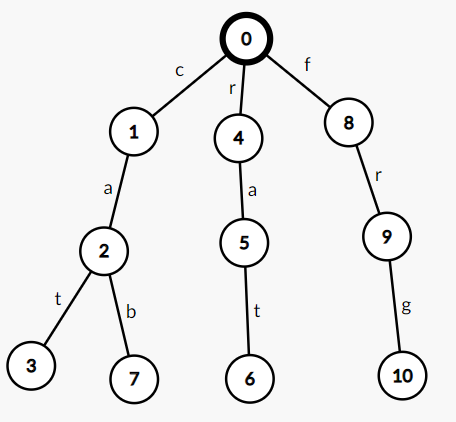
\includegraphics[width=0.4\textwidth,center]{../photo/trie1.png}\\
\indent建立可持久化Trie:\\
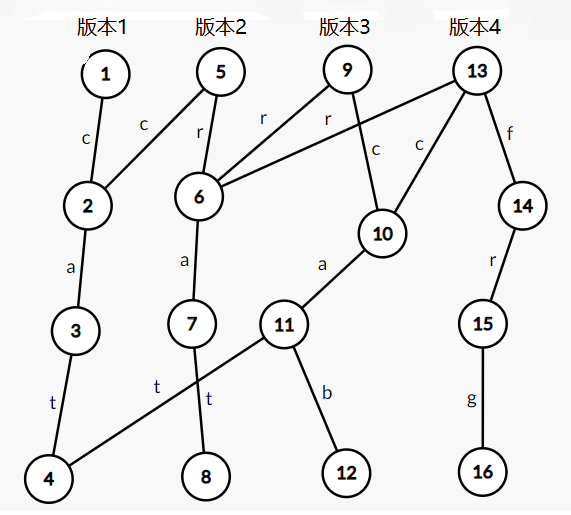
\includegraphics[width=0.4\textwidth,center]{../photo/trie2.png}\\
\begin{lstlisting}[language=c++,escapeinside=``]
void insert(int q,int p,int x)//`将x插入版本p的根中,版本p的上一个版本为版本q`
{
    max_id[q]=x; //`max\_id纪录了该位置下可以找到的最新版本编号`
    for(int i=24;i>=0;i--)
    {
        int u=(sum[x]>>i)&1;
        if(q) trie[p][!u]=trie[q][!u];
        trie[p][u]=++idx;max_id[idx]=x;
        q=trie[q][u],p=idx;
    }
}
void query(int l,int r,int x)//`查询第l个到第r个数字中异或x得到的最大值`
{
    int p=root[r],ans=0;
    for(int i=24;i>=0;i--)
    {
        int u=(x>>i)&1;
        if(trie[p][!u] && max_id[trie[p][!u]]>=l)
        {
            ans+=(1<<i);p=trie[p][!u];
        }
        else p=trie[p][u];
    }
    printf("%d\n",ans);
}
\end{lstlisting}
\section{KMP}
\begin{lstlisting}[language=c++,escapeinside=``]
void getnext(char S[])
{
    int l=strlen(S+1);
    Next[1]=0;
    for(int i=2,k=0;i<=l;i++)
    {
        while(k && S[i]!=S[k+1]) k=Next[k];
        if(S[i]==S[k+1]) k++;
        Next[i]=k;
    }
}
int kmp(char P[],char S[])
{
    int lp=strlen(P+1),ls=strlen(S+1);
    for(int i=1,j=1;i<=lp;i++) //`i为主串指针,j为模式串指针`
    {
        while(j>1 && P[i]!=S[j]) j=Next[j-1]+1;
        if(P[i]==S[j]) j++;
        if(j==ls+1) return i-ls+1;
    }
    return -1;
}
\end{lstlisting}
\subsubsection{Border树}
\indent1.每个前缀Prefix[i]的所有Border:节点i到根的链。\\
\indent2.哪些前缀有长度为$x$的Border:$x$的子树。\\
\indent3.求两个前缀的公共Border等价于求LCA。\\
\subsubsection{字符串的周期}
\indent p是S的周期=$|$S$|-$p是S的Border,S的Border的Border也是S的Border。\\
\subsubsection{统计每个前缀的出现次数}
\indent统计每个前缀Prefix[i]在同一个字符串的出现次数。
\begin{lstlisting}[language=c++,escapeinside=``]
for(int i=1;i<=n;i++) ans[nex[i]]++;
for(int i=n;i>=1;i--) ans[nex[i]]+=ans[i];
for(int i=1;i<=n;i++) ans[i]++;
\end{lstlisting}
\indent考虑第二个问题,字符串S的每个前缀在字符串T中的出现次数是多少。构造字符串S+\#+T,对新字符串长度$\ge n$的部分进行上面的操作即可。\\
\section{拓展KMP}
\begin{lstlisting}[language=c++,escapeinside=``]
// `exkmp(s,n,s,n,nxt,nxt) 求字符串s的Zbox`
// `exkmp(t,m,s,n,ext,nxt) 求字符串t的后缀与s的LCP`
void exkmp(char *s,int lens,char *t,int lent,int *ext,int *nxt)
{
    ext[0]=0;
    for(int i=1,l=0,r=0;i<=lens;i++)
    {
        ext[i]=i<=r?min(nxt[i-l+1],r-i+1):0;
        while(i+ext[i]<=lens && ext[i]<lent && s[i+ext[i]]==t[ext[i]+1]) ext[i]++;
        if(i+ext[i]-1>=r && i!=1) l=i,r=i+ext[i]-1;
    }
}
\end{lstlisting}
\section{AC自动机}
\indent KMP:一个模式串在一个主串上匹配。AC自动机:多个模式串在主串上匹配。\\
\indent1.Trie树构建的复杂度是$O(m\times len)$,其中$m$为模式串数量,$len$为模式串平均长度。\\
\indent2.构建fail指针时,时间也是线性的。\\
\indent3.在匹配时,最耗时的是fail指针的跳动,每次最多前跳$len$次,若主串长度为$n$,那么总匹配时间复杂度为$O(n*len)$。
\begin{lstlisting}[language=c++,escapeinside=``]
void insert(char s[])
{
    int p=0,l=strlen(s);
    for(int i=0;i<l;i++)
    {
        int u=s[i]-'a';
        if(!trie[p][u]) trie[p][u]=++cnt;
        p=trie[p][u];		
    }
    son[p]++;
}
void make_fail()
{
    queue<int>q;
    for(int i=0;i<26;i++)
        if(trie[0][i]) q.push(trie[0][i]);
    while(!q.empty())
    {
        int t=q.front(); q.pop();
        for(int i=0;i<26;i++)
        {
            int p=trie[t][i];
            if(!p) trie[t][i]=trie[fail[t]][i];
            else
            {
                fail[p]=trie[fail[t]][i];
                q.push(p);
            }
        }
    }
}
int query(char s[]) //`查询多少模式串在字符串s中出现过`
{
    int nn=0;
    int num=0,l=strlen(s);
    for(int i=0,j=0;i<l;i++)
    {
        int t=s[i]-'a';j=trie[j][t];
        int p=j;
        while(p && ~son[p])
        {
            nn++;num+=son[p];
            son[p]=-1;p=fail[p];
        }
    }
    return num;
}
\end{lstlisting}
\subsubsection{AC自动机上拓扑排序}
假设当前的位置为$p$,这意味着我们当前匹配到了$p$以及$p$的fail链上的所有位置。所以对fail树进行拓扑排序可较快求解。
\begin{lstlisting}[language=c++]
for(int i=1;i<=cnt;i++) d[fail[i]]++;
for(int i=1;i<=cnt;i++) if(d[i]==0) q.push(i);
while(!q.empty())
{
    int u=q.front();q.pop();
    d[fail[u]]--;ans[fail[u]]+=ans[u];
    if(d[fail[u]]==0) q.push(fail[u]);
}
\end{lstlisting}
\subsubsection{last指针优化}
在自动机上跳fail时,有时不得不遍历一些无用的fail结点,我们将fail链压缩,压缩为只包含关键结点的last指针。时间复杂度为$O(\sqrt n)$。
\subsubsection{AC自动机结合DP}
通常先对son数组进行预处理,常见的有在BFS过程中:son[t]$\mid=$son[fail[t]]或son[t]$+=$son[fail[t]]。
\begin{lstlisting}[language=c++]
for(int i=1;i<=len;i++)
{
    for(int j=0;j<=cnt;j++)
    {
        for(int u=0;u<26;u++)
        {
            f[i][trie[j][u]]=max(f[i][trie[j][u]],f[i-1][j]+son[trie[j][u]]);
            ans=max(ans,f[i][trie[j][u]]);
        }
    }
}
\end{lstlisting}
\subsubsection{fail树上DFS序+数据结构操作}
\indent由于AC自动机属于离线算法,有时候我们会遇到一些需要在线维护更新的题目。将AC自动机上的fail指针全部反过来,就得到了fail树。这种题目一般是利用fail树上的性质,配合数据结构(差分,树状数组,离线,树剖)来变成树论中的数据结构问题。\\
\indent遇到这种问题,首先要想清楚如何在fail树上处理单组询问,不断尝试用数据结构优化即可。\\
\noindent常见数据结构技巧:\\
\indent1.询问某结点子树下的数字之和。使用DFS序将结点映射为序列,$u$结点代表的子树序列为$L[u],R[u]$(入栈时间和出栈时间)。\\
\indent2.将某结点子树下的权值统一加一。可使用上述DFS序用树状数组区间修改。或者使用树状数组维护一个差分数组,$u$结点子树都加一,等于$L[x]$加$1$,$R[x]+1$减$1$。\\
\indent3.将链上的值统一加一。使用树剖。或者用树状数组维护树上差分,差分后某点/边的值等于子树之和,用1求解。
\section{Manacher}
\begin{lstlisting}[language=c++]
int manacher(char S[],int P[],char New[])
{
    int len=0,k=1,l=strlen(S+1);
    New[k]='#';
    for(int i=1;i<=l;i++)
    {
        New[++k]=S[i];New[++k]='#';
    }
    int mx=0,mid;
    for(int i=1;i<=k;i++)
    {
        if(i<mx) P[i]=min(mx-i,P[2*mid-i]);
        else P[i]=1;
        while(i-P[i]>=1 && i+P[i]<=k && New[i-P[i]]==New[i+P[i]]) P[i]++;
        if(i+P[i]>mx)
        {
            mx=i+P[i];mid=i;len=max(len,P[i]);
        }
    }
    return len-1; //找到的最长回文长度
}
\end{lstlisting}
\section{回文自动机}
\indent对于一个字符串$s$,它的本质不同回文子串个数最多只有$|s|$个。因此回文树状态数是$|s|$的。对于每一个状态,它实际只代表一个本质不同的回文子串,即转移到该节点的状态唯一,因此总转移数也是$|s|$的。\\
\indent和其它的自动机一样,一个节点的fail指针指向的是这个节点所代表的\textbf{回文串的最长回文后缀}所对应的节点,但是转移边并非代表在原节点代表的回文串后加一个字符,而是表示在原节点代表的回文串前后各加一个相同的字符。\\
\indent回文树有两个初始状态,分别代表长度为$-1,0$的回文串。我们可以称它们为奇根,偶根。它们不表示任何实际的字符串,仅作为初始状态存在。考虑构造完前$p-1$个字符的回文树后,向自动机中添加在原串里位置为$p$的字符。我们从以上一个字符结尾的最长回文子串对应的节点开始,不断沿着fail指针走,直到找到一个节点p满足s[i]=s[i-len[p]-1],即满足此节点所对应回文子串的上一个字符与待添加字符相同。构造时间复杂度$O(|s|)$\\
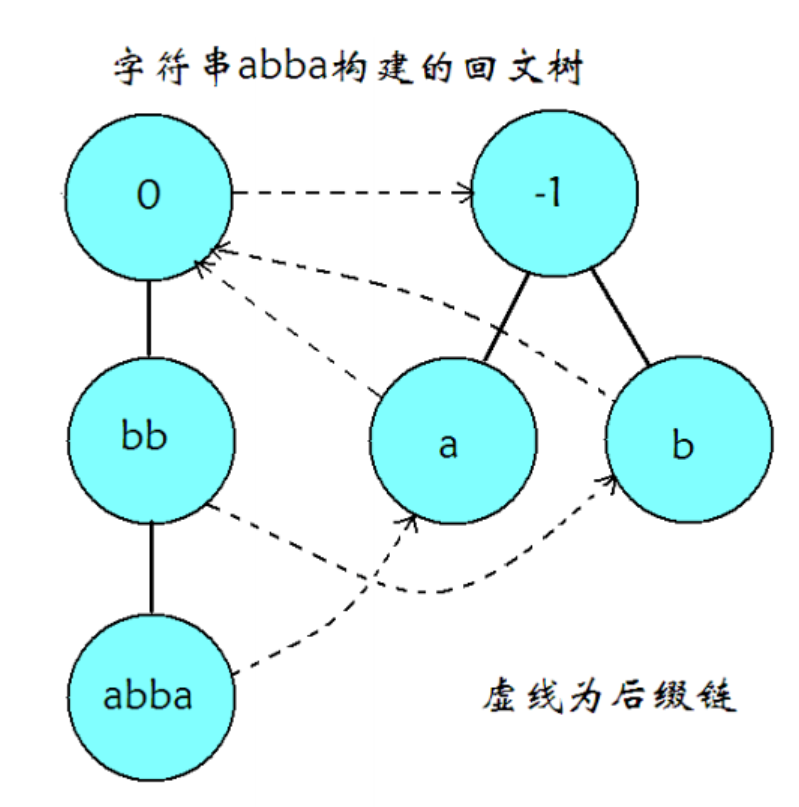
\includegraphics[width=0.4\textwidth,center]{../photo/pam}\\
\begin{lstlisting}[language=c++,escapeinside=``]
struct PAM
{
    int len[maxn],ch[maxn][26],fail[maxn],cnt;
    char s[maxn];
    PAM()
    {
        len[1]=-1;len[0]=0;fail[1]=0;fail[0]=1;cnt=1;
    }
    int get_fail(int x,int i) //`看看x的fail链上哪个可以接上s[i]`
    {
        while(s[i-len[x]-1]!=s[i]) x=fail[x];
        return x;
    }
    void insert()
    {
        int l=strlen(s+1),p=0;
        for(int i=1;i<=l;i++)
        {
            int u=s[i]-'a',pos=get_fail(p,i);
            if(!ch[pos][u])
            {
                fail[++cnt]=ch[get_fail(fail[pos],i)][u];
                ch[pos][u]=cnt;len[cnt]=len[pos]+2;
            }
            p=ch[pos][s[i]-'a'];
        }
    }
}pam;
\end{lstlisting}
\subsubsection{本质不同回文子串个数}
一个串的本质不同回文子串个数等于回文树的状态数(排除奇根和偶根两个状态)。
\subsubsection{回文子串出现次数}
建出回文树,使用类似后缀自动机统计出现次数的方法。由于回文树的构造过程中,节点本身就是按照拓扑序插入,因此只需要逆序枚举所有状态,将当前状态的出现次数加到其fail指针对应状态的出现次数上即可。
\begin{lstlisting}[language=c++]
void build()
{
    for(int i=cnt;i>=0;i--) sz[fail[i]]+=sz[i];
}
\end{lstlisting}
也可以在字符插入的过程维护nump[u]=nump[fail[u]]+1,即求出字符串当前位置结尾的字符串数量,统计插入过程的所有nump[u]之和即可。
\subsubsection{双向插入PAM}
由于回文串的特殊性,PAM在建造时可以从字符串一个位置出发,向左右两边用时插入字符,这需要维护两个结束结点pre和last,当插入字符后发现整个字符串就是一个回文串时,要同时更新pre和last。
\begin{lstlisting}[language=c++]
void insert_front(int x,int c)
{
    while(s[x]!=s[x+len[pre]+1]) pre=fail[pre];
    if (!ch[pre][c]) 
    {
        len[++cnt]=len[pre]+2;
        int j=fail[pre];while(s[x+len[j]+1]!=s[x]) j=fail[j];
        fail[cnt]=ch[j][c];ch[pre][c]=cnt;
        nump[cnt]=nump[fail[cnt]]+1;
    }
    pre=ch[pre][c];
    if(len[pre]==r-l+1) last=pre; //若本身为回文串更新last
    sum=sum+nump[pre]; //所有回文串总数
}
void insert_back(int x,int c)
{
    while(s[x]!=s[x-len[last]-1]) last=fail[last];
    if (!ch[last][c]) 
    {
        len[++cnt]=len[last]+2;
        int j=fail[last];while(s[x-len[j]-1]!=s[x]) j=fail[j];
        fail[cnt]=ch[j][c];ch[last][c]=cnt;
        nump[cnt]=nump[fail[cnt]]+1;
    }
    last=ch[last][c];
    if(len[last]==r-l+1) pre=last; //若本身为回文串更新pre
    sum=sum+nump[last]; //所有回文串总数
}
\end{lstlisting}

\section{后缀数组}
\indent将字符串的所有后缀进行字典序排序,令$sa[i]$代表排名第$i$的后缀字符串的起始位置的下标,$rk[i]$代表从第$i$位开始的后缀字符串的排名,这两个数组满足性质:$sa[rk[i]]=rk[sa[i]]=i$。\\
\subsection{倍增}
\indent使用倍增的思想,先对每个长度为$1$的子串(即每个字符)进行排序。\\
\indent$S[i,k]$表示从$i$开始,长度为$2^k$的字符串,则$S[i,k+1]=S[i,k]+S[i+2^k,k]$。\\
\indent用上一轮排好的顺序,两两组合,进行双关键字排序($pair$排序),即可用长度为$k$的排名推出长度为$k+1$的排名。\\
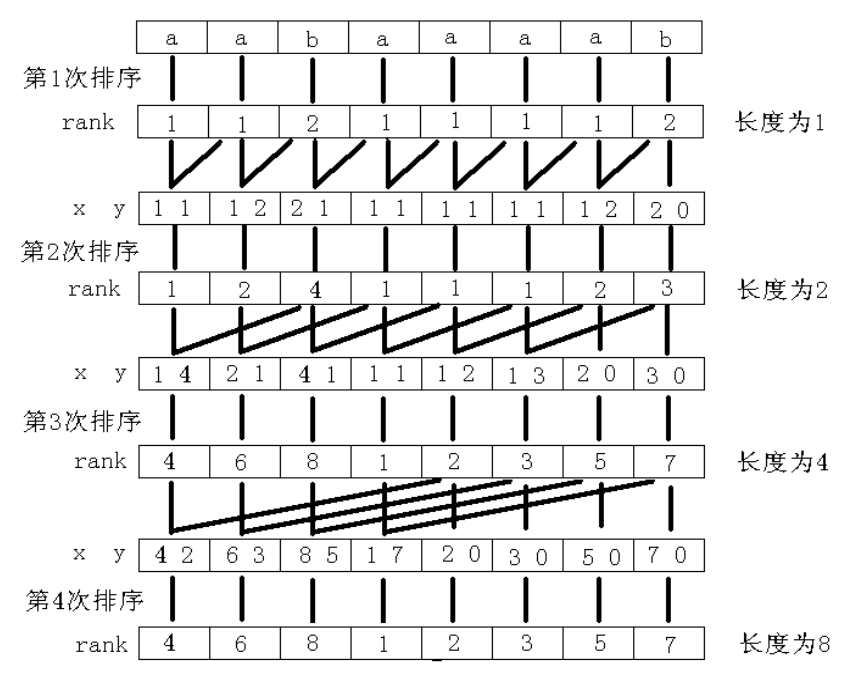
\includegraphics[width=0.7\textwidth,center]{../photo/sa2}\\
\indent如果使用$sort$进行排序,共需排序$\log n$次,时间复杂度$O(n\log ^2n)$,使用基数排序将排序时间优化至$O(n)$,于是总体时间复杂度被优化到了$O(n\log n)$。
\begin{lstlisting}[language=c++,escapeinside=``]
struct Suffix_Array
{
    char s[maxn];
    int n,m=122,x[maxn],y[maxn];
    int rk[maxn],sa[maxn],height[maxn],c[maxn];
    void get_SA() //`记得对n初始化`
    {
        memset(height,0,sizeof(height));
        memset(rk,0,sizeof(rk));
        memset(y,0,sizeof(y));
        for(int i=1;i<=m;i++) c[i]=0;
        for(int i=1;i<=n;i++) c[x[i]=s[i]]++;
        for(int i=1;i<=m;i++) c[i]+=c[i-1];
        for(int i=n;i>=1;i--) sa[c[x[i]]--]=i; //`基数排序先计算出长度为1子串的顺序`
        for(int k=1;k<=n;k<<=1)
        {
            int num=0;
            //`y[i]表示第二关键字排名为i的数,第一关键字的位置`
            //`第n-k+1到第n位是没有第二关键字的,所以排名在最前面`
            for(int i=n-k+1;i<=n;i++) y[++num]=i; 
            for(int i=1;i<=n;i++) if(sa[i]>k) y[++num]=sa[i]-k;
            for(int i=1;i<=m;i++) c[i]=0;
            for(int i=1;i<=n;i++) c[x[i]]++;
            for(int i=1;i<=m;i++) c[i]+=c[i-1];
            //`因为y的顺序是按照第二关键字的顺序来排的`
            //`第二关键字靠后的,在同一个第一关键字桶中排名越靠后`
            for(int i=n;i>=1;i--) sa[c[x[y[i]]]--]=y[i],y[i]=0;
            for(int i=1;i<=n;i++) swap(x[i],y[i]);
            x[sa[1]]=1;num=1; 
            //合并并列排名
            for(int i=2;i<=n;i++) 
           x[sa[i]]=(y[sa[i]]==y[sa[i-1]]&&y[sa[i]+k]==y[sa[i-1]+k])?num:++num;
            if(num==n) break; m=num;
        }
        int k=0;height[1]=0;
        for(int i=1;i<=n;i++) rk[sa[i]]=i;
        for(int i=1;i<=n;i++)
        {	
            if(rk[i]==1) continue;
            if(k) k--;
            int j=sa[rk[i]-1];
            while(i+k<=n&&j+k<=n&&s[i+k]==s[j+k]) k++;
            height[rk[i]]=k;
        }
    }
}s1,s2;
\end{lstlisting}
\subsection{SA-IS}
\begin{lstlisting}[language=c++,escapeinside=``]
struct SAIS
{
    int sa[maxn],rk[maxn],s[maxn*2],op[maxn*2],pos[maxn*2];
    int c1[maxn],c[maxn],ht[maxn];
    char str[maxn];
    #define L(x) sa[c[s[x]]--]=x
    #define R(x) sa[c[s[x]]++]=x
    inline void sa_sort(int *S,int n,int m,int *s,int *op,int tn)
    {
        for(int i=1;i<=n;i++) sa[i]=0;
        for(int i=1;i<=m;i++) c1[i]=0;
        for(int i=1;i<=n;i++) c1[s[i]]++;
        for(int i=2;i<=m;i++) c1[i]+=c1[i-1];
        for(int i=1;i<=m;i++) c[i]=c1[i];
        for(int i=tn;i;i--) L(S[i]);
        for(int i=1;i<=m+1;i++) c[i]=c1[i-1]+1;
        for(int i=1;i<=n;i++)
        if(sa[i]>1 && op[sa[i]-1]) R(sa[i]-1);
        for(int i=1;i<=m;i++) c[i]=c1[i];
        for(int i=n;i;i--)
        if(sa[i]>1 && !op[sa[i]-1]) L(sa[i]-1);
    }
    void SA_IS(int n,int m,int *s,int *op,int *pos)//`m代表字符的范围`
    {
        int tot=0,cnt=0;int *S=s+n;
        op[n]=0;
        for(int i=n-1;i;i--) op[i]=(s[i]!=s[i+1])?s[i]>s[i+1]:op[i+1];
        rk[1]=0;
        for(int i=2;i<=n;i++)
        if(op[i-1]==1 && op[i]==0) pos[++tot]=i,rk[i]=tot;
        else rk[i]=0;
        sa_sort(pos,n,m,s,op,tot);
        int u=0,p=0;
        for(int i=1;i<=n;i++)
        if(rk[sa[i]])
        {
            u=rk[sa[i]];
            if(cnt<=1 || pos[u+1]-pos[u]!=pos[p+1]-pos[p]) ++cnt;
            else
            {
                for(int j=0;j<=pos[u+1]-pos[u];j++)
                if(s[pos[u]+j]!=s[pos[p]+j]||op[pos[u]+j]!=op[pos[p]+j])
                {++cnt;break;}
            }
            S[u]=cnt;
            p=u;
        }
        if(tot!=cnt) SA_IS(tot,cnt,S,op+n,pos+n);
        else for(int i=1;i<=tot;i++) sa[S[i]]=i;
        for(int i=1;i<=tot;i++) S[i]=pos[sa[i]];
        sa_sort(S,n,m,s,op,tot);
    }
    void get_ht(int n) //ht[1]=1
    {
        for(int i=1;i<=n;i++) rk[sa[i]=sa[i+1]]=i;
        for(int i=1,p=0;i<=n;ht[rk[i]]=p,i++)
        if(rk[i]!=1) 
        for(p=p-!!p;sa[rk[i]-1]+p<=n && i+p<=n&&s[i+p]==s[sa[rk[i]-1]+p];p++);
    }
    void Get_SA(int n)
    {
        for(int i=1;i<=n;i++) s[i]=str[i];
        s[++n]=1;SA_IS(n--,122,s,op,pos);//`122为字符串的ASCII码范围`
        get_ht(n);
    }
}sa;
\end{lstlisting}
\subsubsection{寻找最小的循环移动位置}
将字符串$S$复制一份变成$SS$就转化成了后缀排序问题。
\subsubsection{从字符串首尾取字符最小化字典序}
需要在原串后缀与反串后缀构成的集合内比较大小,可以将反串拼接在原串后,并在中间加上一个没出现过的字符(如\#,代码中可以直接使用空字符),求后缀数组,即可$O(1)$完成这一判断。
\subsubsection{LCP(最长公共前缀)}
\indent定义$LCP(i,j)$为$suff(i)$和$suff(j)$的最长公共前缀。那么$height[i]=LCP(sa[i],sa[i-1])$,即第$i$名的后缀与它前一名的后缀的最长公共前缀,$height[1]=0$。\\
\indent$height[rk[i]]\ge height[rk[i-1]]-1$。
\subsubsection{两子串最长公共前缀}
$LCP(sa[i],sa[j])=\min\{height[i+1..j]\}$,于是就转换为了RMQ问题。
\begin{lstlisting}[language=c++]
void get_ST()
{
    for(int i=1;i<=n;i++) st[i][0]=height[i];
    for(int j=1;j<16;j++)
    {
        for(int i=1;i+(1<<(j-1))<=n;i++)
        {
            st[i][j]=min(st[i][j-1],st[i+(1<<(j-1))][j-1]);
        }
    }
}
int LCP(int l,int r)
{
    l=rk[l],r=rk[r];
    if(l>r) swap(l,r); l++;
    int k=log2(r-l+1);
    return min(st[l][k],st[r-(1<<k)+1][k]);
}
\end{lstlisting}
\subsubsection{比较一个字符串的两个子串的大小关系}
\indent假设需要比较的是$A[a..b]$和$B[c..d]$的大小关系。\\
\indent若$LCP(a,c)\ge \min(|A,|B|)$,$A<B \iff |A|<|B|$。否则,$A<B \iff rk[a]<rk[c]$。
\subsubsection{不同子串的数目}
\indent子串就是后缀的前缀,所以可以枚举每个后缀,计算前缀总数,再减掉重复。“前缀总数”其实就是子串个数,为$n(n+1)/2$。\\
\indent如果按后缀排序的顺序枚举后缀,每次新增的子串就是除了与上一个后缀的LCP剩下的前缀。这些前缀一定是新增的,否则会破坏$LCP(sa[i],sa[j])$的性质。只有这些前缀是新增的,因为LCP部分在枚举上一个前缀时计算过了。\\
\indent所以答案为$n(n+1)/2-\displaystyle\sum_{i=2}^{n}height[i]$。
\subsubsection{连续的若干个相同子串}
我们可以枚举连续串的长度$|S|$,按照$|S|$对整个串进行分块,对相邻两块的块首进行LCP与LCS查询。\\
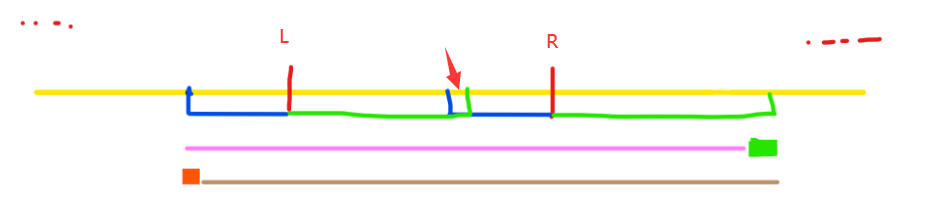
\includegraphics[width=0.7\textwidth,center]{../photo/sa3}\\
\begin{lstlisting}[language=c++,title=字符串多少子串可写成AABB形式]
for(int len=1;len<=n/2;len++)
{
    for(int i=1;i<=n;i+=len)
    {
        int l=i,r=i+len;int lcp=s1.LCP(l,r);lcp=min(lcp,len);
        int L=n-r+2,R=n-l+2;int lcs=s2.LCP(L,R);lcs=min(lcs,len-1);
        if(lcs+lcp>=len)
        {
            int t=lcs+lcp-len;
            b[i-lcs]++;b[i-lcs+t+1]--;
            a[r+lcp-1-t]++;a[r+lcp]--;
        }
    }
}
for(int i=1;i<=n;i++) a[i]+=a[i-1],b[i]+=b[i-1];
ll ans=0; for(int i=1;i<n;i++) ans+=a[i]*b[i+1];
\end{lstlisting}
\subsubsection{结合并查集}
某些题目求解时要求你将后缀数组划分成若干个连续LCP长度大于等于某一值的段,亦即将$h$数组划分成若干个连续最小值大于等于某一值的段并统计每一段的答案。如果有多次询问,我们可以将询问离线。观察到当给定值单调递减的时候,满足条件的区间个数总是越来越少,而新区间都是两个或多个原区间相连所得,且新区间中不包含在原区间内的部分的$h$值都为减少到的这个值。我们只需要维护一个并查集,每次合并相邻的两个区间,并维护统计信息即可。
\subsubsection{结合单调栈}
有些时候我们需要计算$\sum LCP$,使用单调栈,找到每个$height$向左向右可以覆盖的有效范围,直接计算即可。
\begin{lstlisting}[language=c++]
vector<int>st;
for(int i=2;i<=SA.n;i++)
{
    while(!st.empty() && SA.height[st.back()]>SA.height[i]) st.pop_back();
    if(st.empty()) l[i]=1;
    else l[i]=st.back();
    st.pb(i);
}
st.clear();
for(int i=SA.n;i>=2;i--)
{
    while(!st.empty() && SA.height[st.back()]>=SA.height[i]) st.pop_back();
    if(st.empty()) r[i]=SA.n+1;
    else r[i]=st.back();
    st.pb(i);
}
for(int i=2;i<=SA.n;i++) ans+=(r[i]-i)*(i-l[i])*SA.height[i];
\end{lstlisting}
\section{后缀自动机}
在SAM中状态数最多有$2*n-1$个,转移数最多$3n-4$。
\begin{itemize}
    \item $s$的子串可以根据它们结束的位置$\operatorname{endpos}$被划分为多个等价类。
    \item SAM由初始状态$t_0$和与每一个$\operatorname{endpos}$等价类对应的每个状态组成。
    \item 对于每一个状态$v$,一个或多个子串与之匹配。我们记$\operatorname{longest}(v)$为其中最长的一个字符串,记$\operatorname{len}(v)$为它的长度。类似地,记$\operatorname{shortest}(v)$为最短的子串,它的长度为$\operatorname{minlen}(v)$。那么对应这个状态的所有字符串都是字符串$\operatorname{longest}(v)$的不同的后缀,且所有字符串的长度恰好覆盖区间$[\operatorname{minlen}(v),\operatorname{len}(v)]$中的每一个整数。
    \item 对于任意不是$t_0$的状态$v$,定义后缀链接为连接到对应字符串$\operatorname{longest}(v)$的长度为$\operatorname{minlen}(v)-1$的后缀的一条边。从根节点$t_0$出发的后缀链接可以形成一棵树。这棵树也表示$\operatorname{endpos}$集合间的包含关系。
    \item 对于$t_0$以外的状态$v$,可用后缀链接$\operatorname{link}(v)$表达$\operatorname{minlen}(v)$:$\operatorname{minlen}(v)=\operatorname{len}(\operatorname{link}(v))+1$。
    \item 如果我们从任意状态$v_0$开始顺着后缀链接遍历,总会到达初始状态$t_0$。这种情况下我们可以得到一个互不相交的区间$[\operatorname{minlen}(v_i),\operatorname{len}(v_i)]$的序列,且它们的并集形成了连续的区间$[0,\operatorname{len}(v_0)]$。
\end{itemize}
\begin{lstlisting}[language=c++]
struct SAM
{
    int idx,last,len[maxn*2],link[maxn*2],nex[maxn*2][26],sz[maxn*2];
    SAM()
    {
        idx=0;last=0;len[0]=0;link[0]=-1;
    }
    void insert(int c)
    {
        int cur=++idx;
        len[cur]=len[last]+1;sz[cur]=1;
        int p=last;
        while(p!=-1 && !nex[p][c]) nex[p][c]=cur,p=link[p];
        if(p==-1) link[cur]=0;
        else
        {
            int q=nex[p][c];
            if(len[p]+1==len[q]) link[cur]=q;
            else
            {
                int clone=++idx;
                len[clone]=len[p]+1;link[clone]=link[q];sz[clone]=0;
                for(int i=0;i<26;i++) nex[clone][i]=nex[q][i];
                while(p!=-1 && nex[p][c]==q) nex[p][c]=clone,p=link[p];
                link[q]=link[cur]=clone;
            }
        }
        last=cur;
    }
}sam;
\end{lstlisting}
\subsubsection{结点代表的子串出现的次数即字符串上的结尾位置}
\begin{lstlisting}[language=c++]
int c[2*maxn],a[2*maxn];
void build(int n)
{
    int now=1;
    for(int i=1;i<=n;i++) endpos[now=nex[now][s[i]-'a']]=i;
    for(int i=1;i<=idx;i++) c[len[i]]++;
    for(int i=1;i<=n;i++) c[i]+=c[i-1];
    for(int i=idx;i>=1;i--) a[c[len[i]]--]=i;
    for(int i=idx;i>=1;i--) 
    {
        int pos=a[i];sz[link[pos]]+=sz[pos];
        if(!endpos[link[pos]]) endpos[link[pos]]=endpos[pos];
    }
}
\end{lstlisting}
\subsubsection{不同子串个数}
每个节点对应的子串数量是$\operatorname{len}(i)-\operatorname{len}(\operatorname{link}(i))$,对自动机所有节点求和即可。
\subsubsection{所有不同子串的总长度}
每个节点对应的所有后缀长度是$\frac{\operatorname{len}(i)\times(\operatorname{len}(i)+1)}{2}$,减去其$\operatorname{link}$节点的对应值就是该节点的净贡献,对自动机所有节点求和即可。
\subsubsection{字典序第$k$大子串}
字典序第$k$大的子串对应于SAM中字典序第$k$大的路径,因此在计算每个状态的路径数后,我们可以很容易地从SAM的根开始找到第$k$大的路径。预处理的时间复杂度为$O(|S)$,单次查询的复杂度为$O(|ans|\cdot|\Sigma|)$(其中$|ans|$是查询的答案,$|\Sigma|$为字符集的大小)。
\begin{lstlisting}[language=c++,escapeinside=``]
void dfs(int pos,int num)
{
    if(num<=sz[pos]) return;
    num-=sz[pos];
    for(int i=0;i<26;i++)
    {
        int p=nex[pos][i];
        if(!p) continue;
        if(sum[p]<num) num-=sum[p];
        else 
        {
            printf("%c",'a'+i);
            dfs(p,num);return;
        }
    }
}
void build(int n)
{
    for(int i=1;i<=idx;i++) c[len[i]]++;
    for(int i=1;i<=n;i++) c[i]+=c[i-1];
    for(int i=idx;i>=1;i--) a[c[len[i]]--]=i;
    for(int i=idx;i>=1;i--) 
    {
        int pos=a[i];sz[link[pos]]+=sz[pos];
        if(t==0) sz[link[pos]]=1;//`t为0则表示不同位置的相同子串算作一个`
    }
    sz[0]=0;
    for(int i=0;i<=idx;i++) sum[i]=sz[i];
    for(int i=idx;i>=0;i--)
    {
        for(int j=0;j<26;j++)
        {
            int pos=nex[a[i]][j];
            if(!pos) continue;
            sum[a[i]]+=sum[pos];
        }
    }
    if(sum[0]<k){puts("-1");return;}
    dfs(0,k);
}
\end{lstlisting}
\subsubsection{最小循环移位}
容易发现字符串$S+S$包含字符串$S$的所有循环移位作为子串。贪心地访问最小的字符即可。总的时间复杂度为$O(|S|)$。
\subsubsection{两个字符串的最长公共子串}
以其中一个字符串建立SAM,另一个串在SAM上转移。
\begin{lstlisting}
void solve()
{
    scanf("%s",s+1);
    int n=strlen(s+1),p=0,l=0,ans=0;
    for(int i=1;i<=n;i++)
    {
        while(p&&!nex[p][s[i]-'a']) p=link[p],l=len[p];
        if(nex[p][s[i]-'a']) p=nex[p][s[i]-'a'],l++,ans=max(ans,l);
    }
    printf("%d\n",ans);
}
\end{lstlisting}
\subsubsection{多个字符串间的最长公共子串}
以其中一个字符串建立SAM,其余串在SAM上转移。
\begin{lstlisting}[language=c++]
void build()
{
    for(int i=1;i<=idx;i++) c[len[i]]++;
    for(int i=1;i<=idx;i++) c[i]+=c[i-1];
    for(int i=idx;i>=1;i--) a[c[len[i]]--]=i;
}
void solve()
{
    memset(mn,0x3f,sizeof(mn));build();
    while(scanf("%s",s+1)!=EOF)
    {
        int n=strlen(s+1),pos=0,l=0;
        for(int i=1;i<=n;i++)
        {
            while(pos&&!nex[pos][s[i]-'a']) pos=link[pos],l=len[pos];
            if(nex[pos][s[i]-'a']) pos=nex[pos][s[i]-'a'],l++;
            mx[pos]=max(mx[pos],l);
        }
        for(int i=idx;i>=1;i--)
        {
            int now=a[i],fa=link[now];
            mx[fa]=max(mx[fa],min(mx[now],len[fa]));
            mn[now]=min(mn[now],mx[now]);mx[now]=0;
        }
    }
    int ans=0;
    for(int i=1;i<=idx;i++) ans=max(ans,mn[i]);
    printf("%d\n",ans);
}
\end{lstlisting}
\subsubsection{区间本质不同字符串个数}
\begin{lstlisting}[language=c++]
#include<bits/stdc++.h>
using namespace std;
typedef long long ll;
const int maxn = 2e5 + 100;
/* 维护最后出现位置在i(左端点)的本质不同串数量 */
struct SegmentTree_Sum{
    ll Sum[maxn * 8],Lazy[maxn*8];
    void down(int x,int l,int mid,int r){
        Sum[x<<1] += Lazy[x] * (mid - l + 1);
        Sum[x<<1|1] += Lazy[x] * (r - mid);
        Lazy[x<<1] += Lazy[x];
        Lazy[x<<1|1] += Lazy[x];
        Lazy[x] = 0;
    }
    void up(int x){Sum[x] = Sum[x<<1] + Sum[x<<1|1];}
    void update(int x,int l,int r,int L,int R,int val){
        if (l > R or L > r)return;
        if (L <= l and r <= R){
            Sum[x] += 1ll * val * (r - l + 1);
            Lazy[x] += val;
            return;
        }
        int mid = l + r >> 1;down(x,l,mid,r);
        update(x<<1,l,mid,L,R,val);update(x<<1|1,mid+1,r,L,R,val);
        up(x);
    }
    ll query(int x,int l,int r,int L,int R){
        if (l > R or L > r)return 0;
        if (L <= l and r <= R)return Sum[x];
        int mid = l + r >> 1;down(x,l,mid,r);
        return query(x<<1,l,mid,L,R) + query(x<<1|1,mid+1,r,L,R);
    }
}segtree;
struct SegmentTree_Max{
    int Max[maxn*8];
    void update(int x,int l,int r,int pos,int val){
        Max[x] = max(Max[x],val);
        if (l == r)return;
        int mid = l + r >> 1;
        if (pos <= mid)update(x<<1,l,mid,pos,val);
        else update(x<<1|1,mid+1,r,pos,val);
    }
    int query(int x,int l,int r,int L,int R){
        if (l > R or L > r)return -1;
        if (L <= l and r <= R)return Max[x];
        int mid = l + r >> 1;
        return max(query(x<<1,l,mid,L,R),query(x<<1|1,mid+1,r,L,R));
    }
}dfstree;
int n,q;
char s[maxn];
ll ans[maxn];
typedef pair<pair<int,int>,int> Query;
vector<Query> query;
struct Suffix_Automaton{
    int nxt[maxn*2][26],fa[maxn*2],l[maxn*2];
    int last,cnt;
    /* 每个color最上边一个点 */
    int up_to[maxn];
    /* 是否被染过色 */
    bool used[maxn*2];
    Suffix_Automaton(){ clear(); }
    void clear(){
        last =cnt=1;fa[1]=l[1]=0;
        memset(nxt[1],0,sizeof nxt[1]);
    }
    void init(char *s){
        while (*s){add(*s-'a');s++;}
    }
    void add(int c){
        int p = last;
        int np = ++cnt;
        memset(nxt[cnt],0,sizeof nxt[cnt]);
        l[np] = l[p]+1;last = np;
        while (p&&!nxt[p][c])nxt[p][c] = np,p = fa[p];
        if (!p)fa[np]=1;
        else{
            int q = nxt[p][c];
            if (l[q]==l[p]+1)fa[np] =q;
            else{
                int nq = ++ cnt;
                l[nq] = l[p]+1;
                memcpy(nxt[nq],nxt[q],sizeof (nxt[q]));
                fa[nq] =fa[q];fa[np] = fa[q] =nq;
                while (nxt[p][c]==q)nxt[p][c] =nq,p = fa[p];
            }
        }
    }
    vector<int> E[maxn * 2];
    int in[maxn*2],out[maxn*2],dfn;
    void dfs(int u){
        in[u] = ++dfn;
        for (int v:E[u])dfs(v);
        out[u] = dfn;
    }
    void gao(){
        for (int i=2;i<=cnt;i++)E[fa[i]].push_back(i);
        dfs(1);
        for (int i=1,now = 1;i<=n;i++){
            now = nxt[now][s[i] - 'a'];
            assert(l[now] == i);
            segtree.update(1,1,n,1,i,1);
            int u = now;
            while (u != 1 and !used[u]){
                used[u] = true;
                u = fa[u];
            }
            while (u != 1){
                int cur = dfstree.query(1,1,cnt,in[u],out[u]);
                segtree.update(1,1,n,cur - l[u]+1,cur - l[up_to[cur]],-1);
                swap(up_to[cur],u);
            }
            dfstree.update(1,1,cnt,in[now],i);
            up_to[i] = 1;
            while (!query.empty() and query.back().first.second == i){
                int l = query.back().first.first;
                int id = query.back().second;
                ans[id] = segtree.query(1,1,n,l,i);
                query.pop_back();
            }
        }
    }
}sam;
int main(){
    scanf("%s%d",s+1,&q);n=strlen(s+1);
    sam.init(s+1);
    for(int i=1;i<=q;i++){
        int l,r;scanf("%d%d",&l,&r);
        query.push_back({{l,r},i});
    }
    sort(query.begin(),query.end(),[](Query x,Query y){
        return x.first.second > y.first.second;
    });
    sam.gao();
    for(int i=1;i<=q;i++) cout<<ans[i]<<endl;
}
\end{lstlisting}
\section{广义后缀自动机}
后缀自动机是用于处理单个字符串的子串问题的强力工具。而广义后缀自动机则是将后缀自动机整合到字典树中来解决对于多个字符串的子串问题。
\subsection{伪广义后缀自动机}
\begin{enumerate}
    \item 通过用特殊符号将多个串直接连接后,再建立SAM。
    \item 对每个串,重复在同一个SAM上进行建立,每次建立前,将last指针置零。
\end{enumerate}
实现方式简单,而且在面对题目时通常可以达到和广义后缀自动机一样的正确性。但是时间复杂度较为危险。
\subsection{构造广义后缀自动机}
\begin{enumerate}
    \item 将所有字符串插入到字典树中。
    \item 从字典树的根节点开始进行BFS,记录下顺序以及每个节点的父亲节点。
    \item 将得到的BFS序列按照顺序,对每个节点在原字典树上进行构建,注意不能将len小于当前len的数据进行操作。
\end{enumerate}
\indent使用广义后缀自动机解决问题时,建议不要在建立自动机时打标记,最好等自动机建好后遍历字符串打标机,或者直接建立$link$树DFS。
\begin{lstlisting}[language=c++]
struct GSA
{
    int nex[maxn][26],idx,len[maxn*2],link[maxn*2];
    GSA()
    {
        link[0]=-1;
    }
    void insert_trie(char *s)
    {
        int p=0,l=strlen(s+1);
        for(int i=1;i<=l;i++)
        {
            int u=s[i]-'a';
            if(!nex[p][u]) nex[p][u]=++idx;
            p=nex[p][u];
        }
    }
    int insert_sam(int last,int u)
    {
        int cur=nex[last][u];
        if(len[cur]) return cur;
        len[cur]=len[last]+1;
        int p=link[last];
        while(p!=-1 && !nex[p][u]) nex[p][u]=cur,p=link[p];
        if(p==-1) link[cur]=0;
        else 
        {
            int q=nex[p][u];
            if(len[p]+1==len[q]) link[cur]=q;
            else
            {
                int clone=++idx;
                len[clone]=len[p]+1;
                link[clone]=link[q];
                for(int i=0;i<26;i++) 
                    nex[clone][i]=len[nex[q][i]]!=0?nex[q][i]:0;
                while(p!=-1 && nex[p][u]==q) nex[p][u]=clone,p=link[p];
                link[q]=link[cur]=clone;
            }
        }
        return cur;
    }
    void build()
    {
        queue<pair<int,int>>q;
        for(int i=0;i<26;i++) if(nex[0][i]) q.push({0,i});
        while(!q.empty())
        {
            auto item=q.front();q.pop();
            int last=insert_sam(item.first,item.second);
            for(int i=0;i<26;i++) if(nex[last][i]) q.push({last,i});
        }
    }
}sam;
\end{lstlisting}
\section{最小表示法}
\subsubsection{循环同构}
当字符串$S$中可以选定一个位置$i$满足$S[i\cdots n]+S[1\cdots i-1]=T$则称$S$与$T$循环同构。
\subsubsection{最小表示}
字符串$S$的最小表示为与$S$循环同构的所有字符串中字典序最小的字符串。
\subsubsection{算法核心}
考虑对于一对字符串在原字符串$S$中的起始位置分别为$i,j$,且它们的前$k$个字符均相同,即$S[i\cdots i+k-1]=S[j\cdots j+k-1]$。假设$S[i+k]>S[j+j]$,我们发现起始位置下标$l$满足$i\leq l\leq i+k$的字符串均不能成为答案。因为对于任意一个字符串$S_{i+p}$一定存在字符串$S_{j+p}$比它更优。所以我们比较时可以跳过下标$l\in[i,i+k]$, 直接比较$S_{i+k+1}$。时间复杂度$O(n)$。 
\begin{lstlisting}[language=c++]
int minshow()//下标从0开始,方便取模
{
    int k=0,i=0,j=1;
    while(k<n&&i<n&&j<n) 
    {
        if(s[(i+k)%n]==s[(j+k)%n]) k++;
        else 
        {
            s[(i+k)%n]>s[(j+k)%n]?i=i+k+1:j=j+k+1;
            if(i==j) i++; k=0;
        }
    }
    return min(i,j);
}
\end{lstlisting}
\section{Lyndon分解}
\indent对于字符串$S$,如果$S$的字典序严格小于$S$的所有后缀的字典序,我们称$S$为Lyndon串。\\
\indent串$S$的Lyndon分解记为$S=w_1w_2\cdots w_k$,其中所有$w_i$为Lyndon串,并且他们的字典序按照非严格单减排序,即$w_i\ge w_{i+1}$。可以发现,这样的分解存在且唯一。
\subsubsection{Duval算法}
\indent如果一个字符串$t$能够分解为$t=ww\cdots\overline{w}$的形式,其中$w$是一个Lyndon串,而$\overline{w}$是$w$的前缀(可能是空串),那么称$\overline{w}$是近似Lyndon串。一个Lyndon串也是近似Lyndon串。\\
\indent Duval算法运用了贪心的思想。算法过程中我们把串$S$分成三个部分$S=s_1s_2s_3$,其中$s_1$是一个Lyndon串,它的Lyndon分解已经记录;$s_2$是一个近似Lyndon串;$s_3$是未处理的部分。\\
\indent定义一个指针$i$指向$s_2$的首字符,则$i$从$1$遍历到$n$(字符串长度)。在循环的过程中我们定义另一个指针$j$指向$s_3$的首字符,指针$k$指向$s_2$中我们当前考虑的字符(意义是$j$在$s_2$的上一个循环节中对应的字符)。我们的目标是将$s[j]$添加到$s_2$的末尾,这就需要将$s[j]$与$s[k]$做比较:
\begin{enumerate}
    \item 如果$s[j]=s[k]$,则将$s[j]$添加到$s_2$末尾不会影响它的近似简单性。于是我们只需要让指针$j,k$自增(移向下一位)即可。
    \item 如果$s[j]>s[k]$,那么$s_2s[j]$就变成了一个Lyndon串,于是我们将指针$j$自增,而让$k$指向$s_2$的首字符,这样$s_2$就变成了一个循环次数为1的新Lyndon串了。
    \item 如果$s[j]<s[k]$,则$s_2s[j]$就不是一个近似简单串了,那么我们就要把$s_2$分解出它的一个Lyndon子串,这个Lyndon子串的长度将是$j-k$,即它的一个循环节。然后把$s_2$变成分解完以后剩下的部分,继续循环下去(注意,这个情况下我们没有改变指针$j,k$),直到循环节被截完。对于剩余部分,我们只需要将进度「回退」到剩余部分的开头即可。
\end{enumerate}
\indent时间复杂度$O(n)$。
\begin{lstlisting}[language=c++]
vector<string> duval(string s) 
{
    int n=s.size(),i=0;
    vector<string> factorization;
    while(i<n) 
    {
        int j=i+1,k=i;
        while(j<n&&s[k]<=s[j]) 
        {
            if(s[k]<s[j]) k=i;
            else k++;
            j++;
        }
        while(i<=k) 
        {
            factorization.push_back(s.substr(i,j-k));
            i+=j-k;
        }
    }
    return factorization;
}
\end{lstlisting}
\ifx\allfiles\undefined
\end{document}
\fi


    \chapter{计算几何}
    \ifx\allfiles\undefined
\documentclass[a4paper]{book}
\usepackage{ctex}
\usepackage{graphicx} %插入图片
\usepackage{amsmath,amsthm}
\usepackage{lmodern}
\usepackage{float}
\usepackage[export]{adjustbox}
\usepackage{listings,xcolor} %代码块
\usepackage{xcolor}
\usepackage{listings}
\lstset{
    breaklines,                                 % 自动将长的代码行换行排版
    extendedchars=false,                        % 解决代码跨页时,章节标题,页眉等汉字不显示的问题
    backgroundcolor=\color[rgb]{0.96,0.96,0.96},% 背景颜色
    keywordstyle=\color{blue}\bfseries,         % 关键字颜色
    identifierstyle=\color{black},              % 普通标识符颜色
    commentstyle=\color[rgb]{0,0.6,0},          % 注释颜色
    stringstyle=\color[rgb]{0.58,0,0.82},       % 字符串颜色
    showstringspaces=false,                     % 不显示字符串内的空格
    numbers=left,                               % 显示行号
    numberstyle=\small\ttfamily,                % 设置数字字体
    basicstyle=\small\ttfamily,                 % 设置基本字体
    captionpos=t,                               % title在上方(在bottom即为b)
    frame=single,                               % 设置代码框形式
    rulecolor=\color[rgb]{0.8,0.8,0.8},         % 设置代码框颜色
}  
   

\begin{document}
\fi
\begin{lstlisting}[language=c++]
using point_t=long double;  //全局数据类型,可修改为 long long 等

constexpr point_t eps=1e-8;
constexpr long double PI=3.1415926535897932384l;

// 点与向量
template<typename T> struct point
{
    T x,y;

    bool operator==(const point &a) const {return (abs(x-a.x)<=eps && abs(y-a.y)<=eps);}
    bool operator<(const point &a) const {if (abs(x-a.x)<=eps) return y<a.y-eps; return x<a.x-eps;}
    bool operator>(const point &a) const {return !(*this<a || *this==a);}
    point operator+(const point &a) const {return {x+a.x,y+a.y};}
    point operator-(const point &a) const {return {x-a.x,y-a.y};}
    point operator-() const {return {-x,-y};}
    point operator*(const T k) const {return {k*x,k*y};}
    point operator/(const T k) const {return {x/k,y/k};}
    T operator*(const point &a) const {return x*a.x+y*a.y;}  // 点积
    T operator^(const point &a) const {return x*a.y-y*a.x;}  // 叉积,注意优先级
    int toleft(const point &a) const {const auto t=(*this)^a; return (t>eps)-(t<-eps);}  // to-left 测试
    T len2() const {return (*this)*(*this);}  // 向量长度的平方
    T dis2(const point &a) const {return (a-(*this)).len2();}  // 两点距离的平方

    // 涉及浮点数
    long double len() const {return sqrtl(len2());}  // 向量长度
    long double dis(const point &a) const {return sqrtl(dis2(a));}  // 两点距离
    long double ang(const point &a) const {return acosl(max(-1.0l,min(1.0l,((*this)*a)/(len()*a.len()))));}  // 向量夹角
    point rot(const long double rad) const {return {x*cos(rad)-y*sin(rad),x*sin(rad)+y*cos(rad)};}  // 逆时针旋转(给定角度)
    point rot(const long double cosr,const long double sinr) const {return {x*cosr-y*sinr,x*sinr+y*cosr};}  // 逆时针旋转(给定角度的正弦与余弦)
};

using Point=point<point_t>;

// 极角排序
struct argcmp
{
    bool operator()(const Point &a,const Point &b) const
    {
        const auto quad=[](const Point &a)
        {
            if (a.y<-eps) return 1;
            if (a.y>eps) return 4;
            if (a.x<-eps) return 5;
            if (a.x>eps) return 3;
            return 2;
        };
        const int qa=quad(a),qb=quad(b);
        if (qa!=qb) return qa<qb;
        const auto t=a^b;
        // if (abs(t)<=eps) return a*a<b*b-eps;  // 不同长度的向量需要分开
        return t>eps;
    }
};

// 直线
template<typename T> struct line
{
    point<T> p,v;  // p 为直线上一点,v 为方向向量

    bool operator==(const line &a) const {return v.toleft(a.v)==0 && v.toleft(p-a.p)==0;}
    int toleft(const point<T> &a) const {return v.toleft(a-p);}  // to-left 测试
    bool operator<(const line &a) const  // 半平面交算法定义的排序
    {
        if (abs(v^a.v)<=eps && v*a.v>=-eps) return toleft(a.p)==-1;
        return argcmp()(v,a.v);
    }

    // 涉及浮点数
    point<T> inter(const line &a) const {return p+v*((a.v^(p-a.p))/(v^a.v));}  // 直线交点
    long double dis(const point<T> &a) const {return abs(v^(a-p))/v.len();}  // 点到直线距离
    point<T> proj(const point<T> &a) const {return p+v*((v*(a-p))/(v*v));}  // 点在直线上的投影
};

using Line=line<point_t>;

//线段
template<typename T> struct segment
{
    point<T> a,b;

    bool operator<(const segment &s) const {return make_pair(a,b)<make_pair(s.a,s.b);}

    // 判定性函数建议在整数域使用

    // 判断点是否在线段上
    // -1 点在线段端点 | 0 点不在线段上 | 1 点严格在线段上
    int is_on(const point<T> &p) const  
    {
        if (p==a || p==b) return -1;
        return (p-a).toleft(p-b)==0 && (p-a)*(p-b)<-eps;
    }

    // 判断线段直线是否相交
    // -1 直线经过线段端点 | 0 线段和直线不相交 | 1 线段和直线严格相交
    int is_inter(const line<T> &l) const
    {
        if (l.toleft(a)==0 || l.toleft(b)==0) return -1;
        return l.toleft(a)!=l.toleft(b);
    }
    
    // 判断两线段是否相交
    // -1 在某一线段端点处相交 | 0 两线段不相交 | 1 两线段严格相交
    int is_inter(const segment<T> &s) const
    {
        if (is_on(s.a) || is_on(s.b) || s.is_on(a) || s.is_on(b)) return -1;
        const line<T> l{a,b-a},ls{s.a,s.b-s.a};
        return l.toleft(s.a)*l.toleft(s.b)==-1 && ls.toleft(a)*ls.toleft(b)==-1;
    }

    // 点到线段距离
    long double dis(const point<T> &p) const
    {
        if ((p-a)*(b-a)<-eps || (p-b)*(a-b)<-eps) return min(p.dis(a),p.dis(b));
        const line<T> l{a,b-a};
        return l.dis(p);
    }

    // 两线段间距离
    long double dis(const segment<T> &s) const
    {
        if (is_inter(s)) return 0;
        return min({dis(s.a),dis(s.b),s.dis(a),s.dis(b)});
    }
};

using Segment=segment<point_t>;

// 多边形
template<typename T> struct polygon
{
    vector<point<T>> p;  // 以逆时针顺序存储

    size_t nxt(const size_t i) const {return i==p.size()-1?0:i+1;}
    size_t pre(const size_t i) const {return i==0?p.size()-1:i-1;}
    
    // 回转数
    // 返回值第一项表示点是否在多边形边上
    // 对于狭义多边形,回转数为 0 表示点在多边形外,否则点在多边形内
    pair<bool,int> winding(const point<T> &a) const
    {
        int cnt=0;
        for (size_t i=0;i<p.size();i++)
        {
            const point<T> u=p[i],v=p[nxt(i)];
            if (abs((a-u)^(a-v))<=eps && (a-u)*(a-v)<=eps) return {true,0};
            if (abs(u.y-v.y)<=eps) continue;
            const Line uv={u,v-u};
            if (u.y<v.y-eps && uv.toleft(a)<=0) continue;
            if (u.y>v.y+eps && uv.toleft(a)>=0) continue;
            if (u.y<a.y-eps && v.y>=a.y-eps) cnt++;
            if (u.y>=a.y-eps && v.y<a.y-eps) cnt--;
        }
        return {false,cnt};
    }

    // 多边形面积的两倍
    // 可用于判断点的存储顺序是顺时针或逆时针
    T area() const
    {
        T sum=0;
        for (size_t i=0;i<p.size();i++) sum+=p[i]^p[nxt(i)];
        return sum;
    }

    // 多边形的周长
    long double circ() const
    {
        long double sum=0;
        for (size_t i=0;i<p.size();i++) sum+=p[i].dis(p[nxt(i)]);
        return sum;
    }
};

using Polygon=polygon<point_t>;

//凸多边形
template<typename T> struct convex: polygon<T>
{
    // 闵可夫斯基和
    convex operator+(const convex &c) const  
    {
        const auto &p=this->p;
        vector<Segment> e1(p.size()),e2(c.p.size()),edge(p.size()+c.p.size());
        vector<point<T>> res; res.reserve(p.size()+c.p.size());
        const auto cmp=[](const Segment &u,const Segment &v) {return argcmp()(u.b-u.a,v.b-v.a);};
        for (size_t i=0;i<p.size();i++) e1[i]={p[i],p[this->nxt(i)]};
        for (size_t i=0;i<c.p.size();i++) e2[i]={c.p[i],c.p[c.nxt(i)]};
        rotate(e1.begin(),min_element(e1.begin(),e1.end(),cmp),e1.end());
        rotate(e2.begin(),min_element(e2.begin(),e2.end(),cmp),e2.end());
        merge(e1.begin(),e1.end(),e2.begin(),e2.end(),edge.begin(),cmp);
        const auto check=[](const vector<point<T>> &res,const point<T> &u)
        {
            const auto back1=res.back(),back2=*prev(res.end(),2);
            return (back1-back2).toleft(u-back1)==0 && (back1-back2)*(u-back1)>=-eps;
        };
        auto u=e1[0].a+e2[0].a;
        for (const auto &v:edge)
        {
            while (res.size()>1 && check(res,u)) res.pop_back();
            res.push_back(u);
            u=u+v.b-v.a;
        }
        if (res.size()>1 && check(res,res[0])) res.pop_back();
        return {res};
    }

    // 旋转卡壳
    // func 为更新答案的函数,可以根据题目调整位置
    template<typename F> void rotcaliper(const F &func) const
    {
        const auto &p=this->p;
        const auto area=[](const point<T> &u,const point<T> &v,const point<T> &w){return (w-u)^(w-v);};
        for (size_t i=0,j=1;i<p.size();i++)
        {
            const auto nxti=this->nxt(i);
            //func(p[i],p[nxti],p[j]);
            while (area(p[this->nxt(j)],p[i],p[nxti])>=area(p[j],p[i],p[nxti]))
            {
                j=this->nxt(j);
                //func(p[i],p[nxti],p[j]);
            }
            func(p[i],p[nxti],p[j]);
        }
    }

    // 凸多边形的直径的平方
    T diameter2() const
    {
        const auto &p=this->p;
        if (p.size()==1) return 0;
        if (p.size()==2) return p[0].dis2(p[1]);
        T ans=0;
        auto func=[&](const point<T> &u,const point<T> &v,const point<T> &w){ans=max({ans,w.dis2(u),w.dis2(v)});};
        rotcaliper(func);
        return ans;
    }
    // 凸包宽度
	T get_width() const
    {
        T ans=INT_MAX;
        auto func=[&](const point<T> &u,const point<T> &v,const point<T> &w){ans=min({ans,Line{u,v-u}.dis(w)});};
        rotcaliper(func);
        return ans;
    }
    // 最大三角形 n^2 
    T max_triangle() const
    {
        const auto &p=this->p;
        if (p.size()==1) return 0;
        if (p.size()==2) return 0;
        T ans=0;
        auto func=[&](const point<T> &u,const point<T> &v,const point<T> &w){ans=max({ans,(w-u)^(w-v)});};
        rotcaliper(func);
        return ans;
    }
    
    // 判断点是否在凸多边形内
    // 复杂度 O(logn)
    // -1 点在多边形边上 | 0 点在多边形外 | 1 点在多边形内
    int is_in(const point<T> &a) const
    {
        const auto &p=this->p;
        if (p.size()==1) return a==p[0]?-1:0;
        if (p.size()==2) return segment<T>{p[0],p[1]}.is_on(a)?-1:0; 
        if (a==p[0]) return -1;
        if ((p[1]-p[0]).toleft(a-p[0])==-1 || (p.back()-p[0]).toleft(a-p[0])==1) return 0;
        const auto cmp=[&](const Point &u,const Point &v){return (u-p[0]).toleft(v-p[0])==1;};
        const size_t i=lower_bound(p.begin()+1,p.end(),a,cmp)-p.begin();
        if (i==1) return segment<T>{p[0],p[i]}.is_on(a)?-1:0;
        if (i==p.size()-1 && segment<T>{p[0],p[i]}.is_on(a)) return -1;
        if (segment<T>{p[i-1],p[i]}.is_on(a)) return -1;
        return (p[i]-p[i-1]).toleft(a-p[i-1])>0;
    }

    // 凸多边形关于某一方向的极点
    // 复杂度 O(logn)
    // 参考资料:https://codeforces.com/blog/entry/48868
    template<typename F> size_t extreme(const F &dir) const
    {
        const auto &p=this->p;
        const auto check=[&](const size_t i){return dir(p[i]).toleft(p[this->nxt(i)]-p[i])>=0;};
        const auto dir0=dir(p[0]); const auto check0=check(0);
        if (!check0 && check(p.size()-1)) return 0;
        const auto cmp=[&](const Point &v)
        {
            const size_t vi=&v-p.data();
            if (vi==0) return 1;
            const auto checkv=check(vi);
            const auto t=dir0.toleft(v-p[0]);
            if (vi==1 && checkv==check0 && t==0) return 1;
            return checkv^(checkv==check0 && t<=0);
        };
        return partition_point(p.begin(),p.end(),cmp)-p.begin();
    }

    // 过凸多边形外一点求凸多边形的切线,返回切点下标
    // 复杂度 O(logn)
    // 必须保证点在多边形外
    pair<size_t,size_t> tangent(const point<T> &a) const
    {
        const size_t i=extreme([&](const point<T> &u){return u-a;});
        const size_t j=extreme([&](const point<T> &u){return a-u;});
        return {i,j};
    }

    // 求平行于给定直线的凸多边形的切线,返回切点下标
    // 复杂度 O(logn)
    pair<size_t,size_t> tangent(const line<T> &a) const
    {
        const size_t i=extreme([&](...){return a.v;});
        const size_t j=extreme([&](...){return -a.v;});
        return {i,j};
    }
};

using Convex=convex<point_t>;

// 点集的凸包
// Andrew 算法,复杂度 O(nlogn)
Convex convexhull(vector<Point> p)
{
    vector<Point> st;
    sort(p.begin(),p.end());
    const auto check=[](const vector<Point> &st,const Point &u)
    {
        const auto back1=st.back(),back2=*prev(st.end(),2);
        return (back1-back2).toleft(u-back2)<=0;
    };
    for (const Point &u:p)
    {
        while (st.size()>1 && check(st,u)) st.pop_back();
        st.push_back(u);
    }
    size_t k=st.size();
    p.pop_back(); reverse(p.begin(),p.end());
    for (const Point &u:p)
    {
        while (st.size()>k && check(st,u)) st.pop_back();
        st.push_back(u);
    }
    st.pop_back();
    return Convex{st};
}
//最小面积矩形 
double rotcaliper(Polygon &a)
{
    double ans=LONG_LONG_MAX;
    Polygon ansp;
    for (int i=0,j=1,l=-1,r=-1;i<(int)a.p.size();i++)
    {
        while (((a.p[a.nxt(j)]-a.p[i])^(a.p[a.nxt(j)]-a.p[a.nxt(i)]))
        >((a.p[j]-a.p[i])^(a.p[j]-a.p[a.nxt(i)]))) j=a.nxt(j);
        if (l==-1) l=i,r=j;
        Point v={a.p[a.nxt(i)]-a.p[i]};
        v=Point{-v.y,v.x};
        while (v.toleft(a.p[a.nxt(l)]-a.p[l])<=0) l=a.nxt(l);
        while (v.toleft(a.p[a.nxt(r)]-a.p[r])>=0) r=a.nxt(r);
        Line li={a.p[i],a.p[a.nxt(i)]-a.p[i]},lj={a.p[j],a.p[i]-a.p[a.nxt(i)]};
        Line l1={a.p[l],v},lr={a.p[r],v};
        vector<Point> t={li.inter(l1),l1.inter(lj),lj.inter(lr),lr.inter(li)};
        Polygon pl={t};
        double s=pl.area();
        if (s<ans) ans=s,ansp=pl;
    }
    return ans;
}
// 圆
struct Circle
{
    Point c;
    long double r;

    bool operator==(const Circle &a) const {return c==a.c && abs(r-a.r)<=eps;}
    long double circ() const {return 2*PI*r;}  // 周长
    long double area() const {return PI*r*r;}  // 面积

    // 点与圆的关系
    // -1 圆上 | 0 圆外 | 1 圆内
    int is_in(const Point &p) const {const long double d=p.dis(c); return abs(d-r)<=eps?-1:d<r-eps;}

    // 直线与圆关系
    // 0 相离 | 1 相切 | 2 相交
    int relation(const Line &l) const
    {
        const long double d=l.dis(c);
        if (d>r+eps) return 0;
        if (abs(d-r)<=eps) return 1;
        return 2;
    }

    // 圆与圆关系
    // -1 相同 | 0 相离 | 1 外切 | 2 相交 | 3 内切 | 4 内含
    int relation(const Circle &a) const
    {
        if (*this==a) return -1;
        const long double d=c.dis(a.c);
        if (d>r+a.r+eps) return 0;
        if (abs(d-r-a.r)<=eps) return 1;
        if (abs(d-abs(r-a.r))<=eps) return 3;
        if (d<abs(r-a.r)-eps) return 4;
        return 2;
    }

    // 直线与圆的交点
    vector<Point> inter(const Line &l) const
    {
        const long double d=l.dis(c);
        const Point p=l.proj(c);
        const int t=relation(l);
        if (t==0) return vector<Point>();
        if (t==1) return vector<Point>{p};
        const long double k=sqrt(r*r-d*d);
        return vector<Point>{p-(l.v/l.v.len())*k,p+(l.v/l.v.len())*k};
    }

    // 圆与圆交点
    vector<Point> inter(const Circle &a) const
    {
        const long double d=c.dis(a.c);
        const int t=relation(a);
        if (t==-1 || t==0 || t==4) return vector<Point>();
        Point e=a.c-c; e=e/e.len()*r;
        if (t==1 || t==3) 
        {
            if (r*r+d*d-a.r*a.r>=-eps) return vector<Point>{c+e};
            return vector<Point>{c-e};
        }
        const long double costh=(r*r+d*d-a.r*a.r)/(2*r*d),sinth=sqrt(1-costh*costh);
        return vector<Point>{c+e.rot(costh,-sinth),c+e.rot(costh,sinth)};
    }

    // 圆与圆交面积
    long double inter_area(const Circle &a) const
    {
        const long double d=c.dis(a.c);
        const int t=relation(a);
        if (t==-1) return area();
        if (t<2) return 0;
        if (t>2) return min(area(),a.area());
        const long double costh1=(r*r+d*d-a.r*a.r)/(2*r*d),costh2=(a.r*a.r+d*d-r*r)/(2*a.r*d);
        const long double sinth1=sqrt(1-costh1*costh1),sinth2=sqrt(1-costh2*costh2);
        const long double th1=acos(costh1),th2=acos(costh2);
        return r*r*(th1-costh1*sinth1)+a.r*a.r*(th2-costh2*sinth2);
    }

    // 过圆外一点圆的切线
    vector<Line> tangent(const Point &a) const
    {
        const int t=is_in(a);
        if (t==1) return vector<Line>();
        if (t==-1)
        {
            const Point v={-(a-c).y,(a-c).x};
            return vector<Line>{{a,v}};
        }
        Point e=a-c; e=e/e.len()*r;
        const long double costh=r/c.dis(a),sinth=sqrt(1-costh*costh);
        const Point t1=c+e.rot(costh,-sinth),t2=c+e.rot(costh,sinth);
        return vector<Line>{{a,t1-a},{a,t2-a}};
    }

    // 两圆的公切线
    vector<Line> tangent(const Circle &a) const
    {
        const int t=relation(a);
        vector<Line> lines;
        if (t==-1 || t==4) return lines;
        if (t==1 || t==3)
        {
            const Point p=inter(a)[0],v={-(a.c-c).y,(a.c-c).x};
            lines.push_back({p,v});
        }
        const long double d=c.dis(a.c);
        const Point e=(a.c-c)/(a.c-c).len();
        if (t<=2)
        {
            const long double costh=(r-a.r)/d,sinth=sqrt(1-costh*costh);
            const Point d1=e.rot(costh,-sinth),d2=e.rot(costh,sinth);
            const Point u1=c+d1*r,u2=c+d2*r,v1=a.c+d1*a.r,v2=a.c+d2*a.r;
            lines.push_back({u1,v1-u1}); lines.push_back({u2,v2-u2});
        }
        if (t==0)
        {
            const long double costh=(r+a.r)/d,sinth=sqrt(1-costh*costh);
            const Point d1=e.rot(costh,-sinth),d2=e.rot(costh,sinth);
            const Point u1=c+d1*r,u2=c+d2*r,v1=a.c-d1*a.r,v2=a.c-d2*a.r;
            lines.push_back({u1,v1-u1}); lines.push_back({u2,v2-u2});
        }
        return lines;
    }
};

// 圆与多边形面积交
long double area_inter(const Circle &circ,const Polygon &poly)
{
    const auto cal=[](const Circle &circ,const Point &a,const Point &b)
    {
        if ((a-circ.c).toleft(b-circ.c)==0) return 0.0l;
        const auto ina=circ.is_in(a),inb=circ.is_in(b);
        const Line ab={a,b-a};
        if (ina && inb) return ((a-circ.c)^(b-circ.c))/2;
        if (ina && !inb)
        {
            const auto t=circ.inter(ab);
            const Point p=t.size()==1?t[0]:t[1];
            const long double ans=((a-circ.c)^(p-circ.c))/2;
            const long double th=(p-circ.c).ang(b-circ.c);
            const long double d=circ.r*circ.r*th/2;
            if ((a-circ.c).toleft(b-circ.c)==1) return ans+d;
            return ans-d;
        }
        if (!ina && inb)
        {
            const Point p=circ.inter(ab)[0];
            const long double ans=((p-circ.c)^(b-circ.c))/2;
            const long double th=(a-circ.c).ang(p-circ.c);
            const long double d=circ.r*circ.r*th/2;
            if ((a-circ.c).toleft(b-circ.c)==1) return ans+d;
            return ans-d;
        }
        const auto p=circ.inter(ab);
        if (p.size()==2 && Segment{a,b}.dis(circ.c)<=circ.r+eps)
        {
            const long double ans=((p[0]-circ.c)^(p[1]-circ.c))/2;
            const long double th1=(a-circ.c).ang(p[0]-circ.c),th2=(b-circ.c).ang(p[1]-circ.c);
            const long double d1=circ.r*circ.r*th1/2,d2=circ.r*circ.r*th2/2;
            if ((a-circ.c).toleft(b-circ.c)==1) return ans+d1+d2;
            return ans-d1-d2;
        }
        const long double th=(a-circ.c).ang(b-circ.c);
        if ((a-circ.c).toleft(b-circ.c)==1) return circ.r*circ.r*th/2;
        return -circ.r*circ.r*th/2;
    };

    long double ans=0;
    for (size_t i=0;i<poly.p.size();i++)
    {
        const Point a=poly.p[i],b=poly.p[poly.nxt(i)];
        ans+=cal(circ,a,b);
    }
    return ans;
}


// 半平面交
// 排序增量法,复杂度 O(nlogn)
// 输入与返回值都是用直线表示的半平面集合
vector<Line> halfinter(vector<Line> l, const point_t lim=1e9)
{
    const auto check=[](const Line &a,const Line &b,const Line &c){return a.toleft(b.inter(c))<0;};
    // 无精度误差的方法,但注意取值范围会扩大到三次方
    /*const auto check=[](const Line &a,const Line &b,const Line &c)
    {
        const Point p=a.v*(b.v^c.v),q=b.p*(b.v^c.v)+b.v*(c.v^(b.p-c.p))-a.p*(b.v^c.v);
        return p.toleft(q)<0;
    };*/
    l.push_back({{-lim,0},{0,-1}}); l.push_back({{0,-lim},{1,0}});
    l.push_back({{lim,0},{0,1}}); l.push_back({{0,lim},{-1,0}});
    sort(l.begin(),l.end());
    deque<Line> q;
    for (size_t i=0;i<l.size();i++)
    {
        if (i>0 && l[i-1].v.toleft(l[i].v)==0 && l[i-1].v*l[i].v>eps) continue;
        while (q.size()>1 && check(l[i],q.back(),q[q.size()-2])) q.pop_back();
        while (q.size()>1 && check(l[i],q[0],q[1])) q.pop_front();
        if (!q.empty() && q.back().v.toleft(l[i].v)<=0) return vector<Line>();
        q.push_back(l[i]);
    }
    while (q.size()>1 && check(q[0],q.back(),q[q.size()-2])) q.pop_back();
    while (q.size()>1 && check(q.back(),q[0],q[1])) q.pop_front();
    return vector<Line>(q.begin(),q.end());
}

// 点集形成的最小最大三角形
// 极角序扫描线,复杂度 O(n^2logn)
// 最大三角形问题可以使用凸包与旋转卡壳做到 O(n^2)
pair<point_t,point_t> minmax_triangle(const vector<Point> &vec)
{
    if (vec.size()<=2) return {0,0};
    vector<pair<int,int>> evt;
    evt.reserve(vec.size()*vec.size());
    point_t maxans=0,minans=numeric_limits<point_t>::max();
    for (size_t i=0;i<vec.size();i++)
    {
        for (size_t j=0;j<vec.size();j++)
        {
            if (i==j) continue;
            if (vec[i]==vec[j]) minans=0;
            else evt.push_back({i,j});
        }
    }
    sort(evt.begin(),evt.end(),[&](const pair<int,int> &u,const pair<int,int> &v)
    {
        const Point du=vec[u.second]-vec[u.first],dv=vec[v.second]-vec[v.first];
        return argcmp()({du.y,-du.x},{dv.y,-dv.x});
    });
    vector<size_t> vx(vec.size()),pos(vec.size());
    for (size_t i=0;i<vec.size();i++) vx[i]=i;
    sort(vx.begin(),vx.end(),[&](int x,int y){return vec[x]<vec[y];});
    for (size_t i=0;i<vx.size();i++) pos[vx[i]]=i;
    for (auto [u,v]:evt)
    {
        const size_t i=pos[u],j=pos[v];
        const size_t l=min(i,j),r=max(i,j);
        const Point vecu=vec[u],vecv=vec[v];
        if (l>0) minans=min(minans,abs((vec[vx[l-1]]-vecu)^(vec[vx[l-1]]-vecv)));
        if (r<vx.size()-1) minans=min(minans,abs((vec[vx[r+1]]-vecu)^(vec[vx[r+1]]-vecv)));
        maxans=max({maxans,abs((vec[vx[0]]-vecu)^(vec[vx[0]]-vecv)),abs((vec[vx.back()]-vecu)^(vec[vx.back()]-vecv))});
        if (i<j) swap(vx[i],vx[j]),pos[u]=j,pos[v]=i;
    }
    return {minans,maxans};
}

// 判断多条线段是否有交点
// 扫描线,复杂度 O(nlogn)
bool segs_inter(const vector<Segment> &segs)
{
    if (segs.empty()) return false;
    using seq_t=tuple<point_t,int,Segment>;
    const auto seqcmp=[](const seq_t &u, const seq_t &v)
    {
        const auto [u0,u1,u2]=u;
        const auto [v0,v1,v2]=v;
        if (abs(u0-v0)<=eps) return make_pair(u1,u2)<make_pair(v1,v2);
        return u0<v0-eps;
    };
    vector<seq_t> seq;
    for (auto seg:segs)
    {
        if (seg.a.x>seg.b.x+eps) swap(seg.a,seg.b);
        seq.push_back({seg.a.x,0,seg});
        seq.push_back({seg.b.x,1,seg});
    }
    sort(seq.begin(),seq.end(),seqcmp);
    point_t x_now;
    auto cmp=[&](const Segment &u, const Segment &v)
    {
        if (abs(u.a.x-u.b.x)<=eps || abs(v.a.x-v.b.x)<=eps) return u.a.y<v.a.y-eps;
        return ((x_now-u.a.x)*(u.b.y-u.a.y)+u.a.y*(u.b.x-u.a.x))*(v.b.x-v.a.x)<((x_now-v.a.x)*(v.b.y-v.a.y)+v.a.y*(v.b.x-v.a.x))*(u.b.x-u.a.x)-eps;
    };
    multiset<Segment,decltype(cmp)> s{cmp};
    for (const auto [x,o,seg]:seq)
    {
        x_now=x;
        const auto it=s.lower_bound(seg);
        if (o==0)
        {
            if (it!=s.end() && seg.is_inter(*it)) return true;
            if (it!=s.begin() && seg.is_inter(*prev(it))) return true;
            s.insert(seg);
        }
        else
        {
            if (next(it)!=s.end() && it!=s.begin() && (*prev(it)).is_inter(*next(it))) return true;
            s.erase(it);
        }
    }
    return false;
}

// 多边形面积并
// 轮廓积分,复杂度约 O(边数^2)
// ans[i] 表示被至少覆盖了 i+1 次的区域的面积
vector<long double> area_union(const vector<Polygon> &polys)
{
    const size_t siz=polys.size();
    vector<vector<pair<Point,Point>>> segs(siz);
    const auto check=[](const Point &u,const Segment &e){return !((u<e.a && u<e.b) || (u>e.a && u>e.b));};
    auto cut_edge=[&](const Segment &e,const size_t i)
    {
        const Line le{e.a,e.b-e.a};
        const auto cmp=[&](const Point &u,const Point &v){return e.a<e.b?u<v:u>v;};
        map<Point,int,decltype(cmp)> cnt(cmp);
        cnt[e.a]; cnt[e.b];
        for (size_t j=0;j<polys.size();j++)
        {
            if (i==j) continue;
            const auto &pj=polys[j];
            for (size_t k=0;k<pj.p.size();k++)
            {
                const Segment s={pj.p[k],pj.p[pj.nxt(k)]};
                if (le.toleft(s.a)==0 && le.toleft(s.b)==0) cnt[s.a],cnt[s.b];
                else if (s.is_inter(le))
                {
                    const Line ls{s.a,s.b-s.a};
                    const Point u=le.inter(ls);
                    if (le.toleft(s.a)<0 && le.toleft(s.b)>=0) cnt[u]--;
                    else if (le.toleft(s.a)>=0 && le.toleft(s.b)<0) cnt[u]++;
                }
            }
        }
        int sum=cnt.begin()->second;
        for (auto it=cnt.begin();next(it)!=cnt.end();it++)
        {
            const Point u=it->first,v=next(it)->first;
            if (check(u,e) && check(v,e)) segs[sum].push_back({u,v});
            sum+=next(it)->second;
        }
    };
    for (size_t i=0;i<polys.size();i++)
    {
        const auto &pi=polys[i];
        for (size_t k=0;k<pi.p.size();k++)
        {
            const Segment ei={pi.p[k],pi.p[pi.nxt(k)]};
            cut_edge(ei,i);
        }
    }
    vector<long double> ans(siz);
    for (size_t i=0;i<siz;i++)
    {
        long double sum=0;
        sort(segs[i].begin(),segs[i].end());
        int cnt=0;
        for (size_t j=0;j<segs[i].size();j++)
        {
            if (j>0 && segs[i][j]==segs[i][j-1]) segs[i+(++cnt)].push_back(segs[i][j]);
            else cnt=0,sum+=segs[i][j].first^segs[i][j].second;
        }
        ans[i]=sum/2;
    }
    return ans;
}

// 圆面积并
// 轮廓积分,复杂度约 O(n^2)
// ans[i] 表示被至少覆盖了 i+1 次的区域的面积
vector<long double> area_union(const vector<Circle> &circs)
{
    const size_t siz=circs.size();
    using arc_t=tuple<Point,long double,long double,long double>;
    vector<vector<arc_t>> arcs(siz);

    auto cut_circ=[&](const Circle &ci,const size_t i)
    {
        auto cmp=[](const long double x,const long double y){return x<y-eps;};
        map<long double,int,decltype(cmp)> cnt{cmp}; cnt[-PI]; cnt[PI];
        int init=0;
        for (size_t j=0;j<circs.size();j++)
        {
            if (i==j) continue;
            const Circle &cj=circs[j];
            if (ci.r<cj.r-eps && ci.relation(cj)>=3) init++;
            const auto inters=ci.inter(cj);
            if (inters.size()==1) cnt[atan2l((inters[0]-ci.c).y,(inters[0]-ci.c).x)];
            if (inters.size()==2)
            {
                const Point dl=inters[0]-ci.c,dr=inters[1]-ci.c;
                long double argl=atan2l(dl.y,dl.x),argr=atan2l(dr.y,dr.x);
                if (abs(argl+PI)<=eps) argl=PI;
                if (abs(argr+PI)<=eps) argr=PI;
                if (argl>argr+eps) cnt[argl]++,cnt[PI]--,cnt[-PI]++,cnt[argr]--,init++;
                else cnt[argl]++,cnt[argr]--;
            }
        }
        if (cnt.empty()) arcs[init].push_back({ci.c,ci.r,-PI,PI});
        else
        {
            int sum=init;
            for (auto it=cnt.begin();next(it)!=cnt.end();it++)
            {
                arcs[sum].push_back({ci.c,ci.r,it->first,next(it)->first});
                sum+=next(it)->second;
            }
        }
    };

    for (size_t i=0;i<circs.size();i++)
    {
        const auto &ci=circs[i];
        cut_circ(ci,i);
    }
    vector<long double> ans(siz);
    const auto oint=[](const arc_t &arc)
    {
        const auto [cc,cr,l,r]=arc;
        if (abs(r-l-PI-PI)<=eps) return 2.0l*PI*cr*cr;
        return cr*cr*(r-l)+cc.x*cr*(sin(r)-sin(l))-cc.y*cr*(cos(r)-cos(l));
    };
    for (size_t i=0;i<siz;i++)
    {
        long double sum=0;
        sort(arcs[i].begin(),arcs[i].end());
        int cnt=0;
        for (size_t j=0;j<arcs[i].size();j++)
        {
            if (j>0 && arcs[i][j]==arcs[i][j-1]) arcs[i+(++cnt)].push_back(arcs[i][j]);
            else cnt=0,sum+=oint(arcs[i][j]);
        }
        ans[i]=sum/2;
    }
    return ans;
}
\end{lstlisting}


\ifx\allfiles\undefined
\end{document}
\fi


    \chapter{杂项}
    \ifx\allfiles\undefined
\documentclass[a4paper]{book}
\usepackage{ctex}
\usepackage{graphicx} %插入图片
\usepackage{amsmath,amsthm}
\usepackage{lmodern}
\usepackage{float}
\usepackage[export]{adjustbox}
\usepackage{listings,xcolor} %代码块
\usepackage{xcolor}
\usepackage{listings}
\lstset{
    breaklines,                                 % 自动将长的代码行换行排版
    extendedchars=false,                        % 解决代码跨页时,章节标题,页眉等汉字不显示的问题
    backgroundcolor=\color[rgb]{0.96,0.96,0.96},% 背景颜色
    keywordstyle=\color{blue}\bfseries,         % 关键字颜色
    identifierstyle=\color{black},              % 普通标识符颜色
    commentstyle=\color[rgb]{0,0.6,0},          % 注释颜色
    stringstyle=\color[rgb]{0.58,0,0.82},       % 字符串颜色
    showstringspaces=false,                     % 不显示字符串内的空格
    numbers=left,                               % 显示行号
    numberstyle=\small\ttfamily,                % 设置数字字体
    basicstyle=\small\ttfamily,                 % 设置基本字体
    captionpos=t,                               % title在上方(在bottom即为b)
    frame=single,                               % 设置代码框形式
    rulecolor=\color[rgb]{0.8,0.8,0.8},         % 设置代码框颜色
}  
   

\begin{document}
\fi
\section{快读}
\begin{lstlisting}[language=c++]
int read()
{
    int x=0,f=1;
    char ch=getchar();
    while(ch<48|ch>57)
    {
        if(ch=='-') f=-1;
        ch=getchar();
    }
    while(ch>=48&&ch<=57) x=x*10+ch-48,ch=getchar();
    return x*f;
}
\end{lstlisting}
\section{三分法}
\subsection{整数三分}
\begin{lstlisting}[language=c++,escapeinside=``]
int l,r;
while(r-l>10) 
{
    int midl=l+(r-l)/3,midr=r-(r-l)/3;
    if(check(midl)<=check(midr)) l=midl; //`这里是求凸性函数;如果求凹形,那么改为r=midr`
    else r=midr;
}
int res=1e9;
for(int i=l;i<=r;i++) res=min(res,check(i)); //`找到[l, r]区间的范围` 
\end{lstlisting}
\subsection{浮点三分}
\begin{lstlisting}[language=c++]
double l,r;
while(r-l>1e-8) 
{
    double midl=l+(r-l)/3,midr=r-(r-l)/3;
    if(check(midl)<=check(midr)) l=midl; //这里是求凸性函数;如果求凹形,那么改为r=midr
    else r=midr;
}
\end{lstlisting}
\section{反悔贪心}
\begin{lstlisting}[language=c++,title=种树]
#include<bits/stdc++.h>
#define int long long
using namespace std;
const int maxn=5e5+7;
int n,k,a[maxn],pre[maxn],nex[maxn],vis[maxn],ans=0;
priority_queue<pair<int,int>>q;
void del(int x)
{
    pre[nex[x]]=pre[x];
    nex[pre[x]]=nex[x];
    vis[x]=1;
}
int gready()
{
    int res;
    while(vis[q.top().second]) q.pop();
    int u=q.top().second;
    q.pop();
    res=a[u];
    a[u]=-a[u]+a[pre[u]]+a[nex[u]];
    q.push({a[u],u});
    del(nex[u]);del(pre[u]);
    return res;
}
signed main()
{
    scanf("%lld%lld",&n,&k);
    for(int i=1;i<=n;i++) scanf("%lld",&a[i]),q.push({a[i],i});
    if(k*2>n)
    {
        puts("Error!");return 0;
    }
    for(int i=1;i<=n;i++) pre[i]=i-1,nex[i]=i+1;
    pre[1]=n;nex[n]=1;
    for(int i=1;i<=k;i++) 
    {
        int res=gready();ans+=res;
    }
    printf("%lld\n",ans);
}
\end{lstlisting}
\section{悬线法}
\begin{lstlisting}[language=c++,title=最大的1组成的矩阵的面积]
for(int i=1;i<=n;i++)
{
    for(int j=1;j<=m;j++)
    {
        l[i][j]=j,r[i][j]=j,up[i][j]=a[i][j];
    }
}
for(int i=1;i<=n;i++)
{
    for(int j=1;j<=m;j++)
    {
        if(j!=1&&a[i][j]==1&&a[i][j-1]==1) l[i][j]=l[i][j-1];
    }
    for(int j=m;j>=1;j--)
    {
        if(j!=m&&a[i][j]==1&&a[i][j+1]==1) r[i][j]=r[i][j+1];
    }
}
for(int i=1;i<=n;i++)
{
    for(int j=1;j<=m;j++)
    {
        if(i!=1&&a[i][j]==1&&a[i-1][j]==1)
        {
            r[i][j]=min(r[i][j],r[i-1][j]);
            l[i][j]=max(l[i][j],l[i-1][j]);
            up[i][j]=max(up[i][j],up[i-1][j]+1);
        }
        ans=max(ans,(r[i][j]-l[i][j]+1)*up[i][j]);
    }
}
printf("%d\n",ans);
\end{lstlisting}
\section{分数规划}
\indent给出$a_i$和$b_i$,求一组$w_i\in\{0,1\}$,最小化或最大化。
$$
\displaystyle\frac{\displaystyle\sum_{i=1}^{n}a_i\times w_i}{\displaystyle\sum_{i=1}^{n}b_i\times w_i}
$$
\indent另外一种描述:每种物品有两个权值$a$和$b$,选出若干个物品使得$\frac{\sum a}{\sum b}$最小/最大。\\
\indent分数规划问题的通用方法是二分。假设我们要求最大值。二分一个答案$mid$,然后推式子(为了方便少写了上下界):\\
$$
\begin{aligned}
&\displaystyle\frac{\displaystyle\sum_{i=1}^{n}a_i\times w_i}{\displaystyle\sum_{i=1}^{n}b_i\times w_i}>mid\\
\Longrightarrow&\sum a_i\times w_i-mid\times\sum b_i\times w_i>0\\
\Longrightarrow&\sum w_i\times(a_i-mid\times b_i)>0
\end{aligned}
$$
\begin{lstlisting}[language=c++,escapeinside=``]
bool check(double mid) 
{
    double s=0;
    for(int i=1;i<=n;i++)
        if(a[i]-mid*b[i]>0)  // `如果权值大于0`
            s+=a[i]-mid*b[i];   // `选这个物品`
    return s > 0;
}
\end{lstlisting}
\section{约瑟夫问题}
\indent$n$个人标号$0,1,\cdots,n-1$。逆时针站一圈,从$0$号开始,每一次从当前的人逆时针数$K$个,然后让这个人出局。问最后剩下的人是谁。
\subsubsection{线性算法}
设$J_{n,k}$表示规模分别为$n,k$的约瑟夫问题的答案。我们有如下递归式
$$
J_{(n,k)}=(J_{(n-1,k)}+k)\bmod n
$$
这个也很好推。你从$0$开始数$k$个,让第$k-1$个人出局后剩下$n-1$个人,你计算出在$n-1$个人中选的答案后,再加一个相对位移$k$得到真正的答案。这个算法的复杂度显然是$O(n)$的。
\begin{lstlisting}[language=c++]
int josephus(int n,int k) 
{
    int res=0;
    for(int i=1;i<=n;i++) res=(res+k)%i;
    return res;
}
\end{lstlisting}
\subsubsection{对数算法}
\indent对于$k$较小$n$较大的情况,本题还有一种复杂度为$O(k\log n)$的算法。\\
\indent考虑到我们每次走$k$个删一个,那么在一圈以内我们可以删掉$\left\lfloor\frac{n}{k}\right\rfloor$个,然后剩下了$n-\left\lfloor\frac{n}{k}\right\rfloor$个人。这时我们在第$\left\lfloor\frac{n}{k}\right\rfloor\times k$个人的位置上。而你发现它等于$n-n\bmod k$。于是我们继续递归处理,算完后还原它的相对位置。还原相对位置的依据是:每次做一次删除都会把数到的第$k$个人删除,他们的编号被之后的人逐个继承,也即用$n-\left\lfloor\frac{n}{k}\right\rfloor$人环算时每$k$个人即有$1$个人的位置失算,因此在得数小于$0$时,用还没有被删去$k$倍数编号的$n$人环的$n$求模,在得数大于等于$0$时,即可以直接乘$\frac{k}{k-1}$, 于是得到如下的算法:
\begin{lstlisting}[language=c++]
int josephus(int n,int k) 
{
    if(n==1) return 0;
    if(k==1) return n-1;
    if(k>n) return(josephus(n-1,k)+k)%n; //线性算法
    int res=josephus(n-n/k,k);
    res-=n%k;
    if(res<0) res+=n; //mod n
    else res+=res/(k-1); //还原位置
    return res;
}
\end{lstlisting}
\section{格雷码}
格雷码是一个二进制数系,其中两个相邻数的二进制位只有一位不同。举个例子,$3$位二进制数的格雷码序列为
$$
000,001,011,010,110,111,101,100
$$
注意序列的下标我们以$0$为起点,也就是说$G(0)=000,G(4)=110$。
\begin{lstlisting}[language=c++]
int g(int n){return n^(n>>1);}
\end{lstlisting}
\subsubsection{镜像构造}
$k$位的格雷码可以从$k-1$位的格雷码以上下镜射后加上新位的方式快速得到,如下图:\\
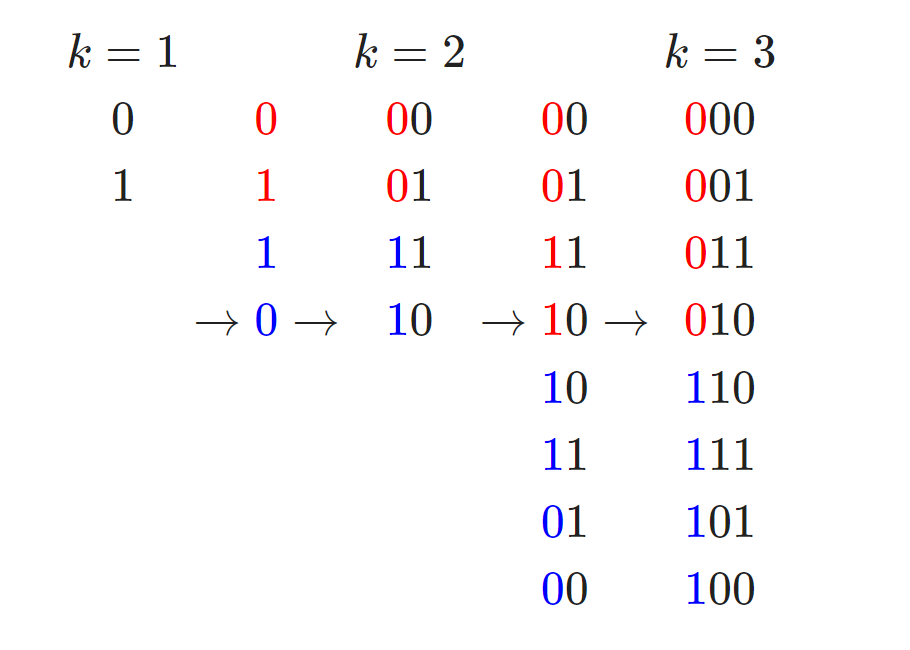
\includegraphics[width=0.5\textwidth,center]{../photo/gray.png}
\subsubsection{格雷码矩阵}
每次拓展两位,向三个方向镜像构造并分别用$01,10,11$作为开头:
$$
\begin{matrix}
0 \\
\end{matrix}\to
\begin{matrix}
00& 10\\ 
01& 11 \\
\end{matrix}\to
\begin{matrix}
0000& 0010& 1010& 1000 \\
0001& 0011& 1011& 1001 \\
0101& 0111& 1111& 1101 \\
0100& 0110& 1110& 1100 \\
\end{matrix}
$$
\subsubsection{通过格雷码构造原数(逆变换)}
\begin{lstlisting}[language=c++]
int rev_g(int g) 
{
    int n=0;
    for(;g;g>>=1) n^=g;
    return n;
}
\end{lstlisting}
\subsubsection{实际应用}
\begin{enumerate}
    \item 格雷码被用于最小化数字模拟转换器(比如传感器)的信号传输中出现的错误,因为它每次只改变一个位。
\end{enumerate}
\section{Zobrist哈希}
\indent Zobrist哈希是一种专门针对棋类游戏而提出来的编码方式。\\
\indent(1)对每个状态的各种情况都生成一个$64$位的数字。\\
\indent(2)将这些数字做异或操作,得到的数字即为哈希值。
\begin{lstlisting}[language=c++,escapeinside=``]
mt19937_64 mrand(random_device{}());//`64位数字随机生成`
\end{lstlisting}
$2X2$的围棋棋盘一共有$4$个单位,每个单位有$3$种状态(黑子,白子,空点),则为每种状态生成$1$个$8$位的随机数:
\begin{center}
    \begin{tabular}{|c|c|c|c|}
    \hline 
    位置 & 黑棋 & 白棋 & 空点\\
    \hline 
    (0,0) & 49 & 189 & 223\\
    \hline 
    (0,1) & 82 & 225 & 50 \\
    \hline 
    (1,0) & 52 & 120 & 65\\
    \hline
    (1,1) & 218 & 34 & 63 \\
    \hline
    \end{tabular}    
\end{center}
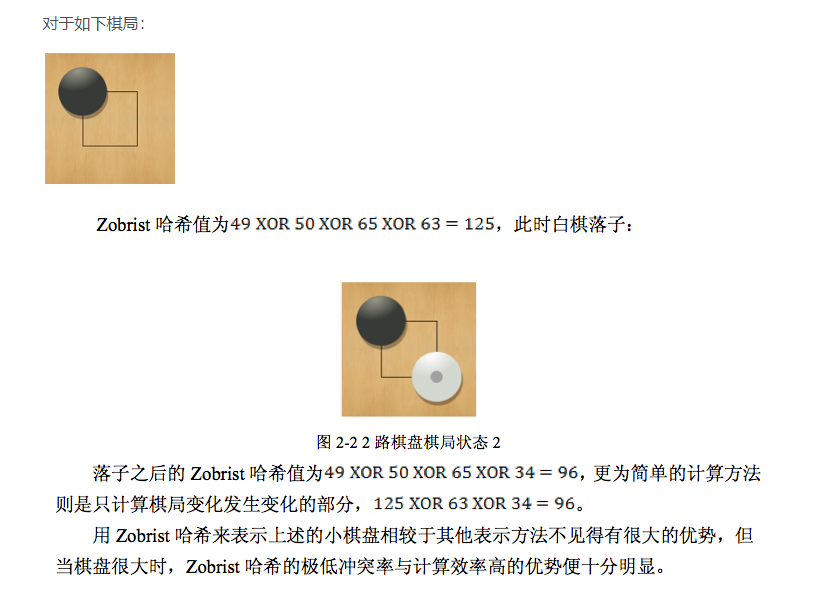
\includegraphics[width=1\textwidth,center]{../photo/zbh}
\section{石子合并}
\begin{lstlisting}[language=c++]
#include <bits/stdc++.h>
using namespace std;
typedef long long ll;
const ll maxn=40005;
ll n,a[maxn],ans,now=1,pro;
int main()
{
	scanf("%lld",&n);
	for(int i=1;i<=n;i++) scanf("%lld",&a[i]);
	while(now<n-1)
	{
		for(pro=now;pro<n-1;pro++)
		{
			if(a[pro+2]<a[pro]) continue;
			a[pro+1]+=a[pro];
            ans+=a[pro+1];ll k;
			for(k=pro;k>now;k--) a[k]=a[k-1]; 
            now++; k=pro+1;
			while(now<k&&a[k-1]<a[k]) {a[k]^=a[k-1]^=a[k]^=a[k-1];k--;}
			break;
		}
		if(pro==n-1) {a[n-1]+=a[n];ans+=a[n-1];n--;}
	}
	if(now==n-1) ans+=(a[n-1]+a[n]); 
    printf("%lld\n",ans);
}
\end{lstlisting}
\section{STL}
\subsection{\_\_int128}
\begin{lstlisting}[language=c++]
__int128 read() //1e36
{
    __int128 x=0,f=1;
    char ch=getchar();
    while(!isdigit(ch)&&ch!='-') ch=getchar();
    if(ch=='-')f=-1;
    while(isdigit(ch))x=x*10+ch-'0',ch=getchar();
    return f*x;
}
void print(__int128 x)
{
    if(x<0)putchar('-'),x=-x;
    if(x>9)print(x/10); 
    putchar(x%10+'0');
}
\end{lstlisting}
\ifx\allfiles\undefined
\end{document}
\fi

\end{document}